% Eriq Augustine
%
% Cal Poly Thesis
%
% based on UC Thesis format
%
% modified by Mark Barry 2/07.
%

% TODO(eriq): Final check for ch/section reference.

\documentclass[12pt]{ucthesis}

\usepackage[hyphens]{url}
\usepackage{hyperref}
\usepackage{subfig}
\usepackage{graphicx}
\usepackage{amssymb}
\usepackage{amsmath}
\usepackage[letterpaper]{geometry}
\usepackage[overload]{textcase}
\usepackage{color}
\usepackage[nonumberlist,toc]{glossaries}
\usepackage{wrapfig}
\usepackage{longtable}
\usepackage{morefloats}
\usepackage{float}
\usepackage{listings}
\usepackage{makecell}

\definecolor{orange}{rgb}{1,0.5,0}
\definecolor{blue}{rgb}{0.1,0.1,0.8}
\definecolor{green}{rgb}{0,0.5,0}
\definecolor{red}{rgb}{0.8,0,0}
\definecolor{bad}{rgb}{0.8,0,0.8}

\makeindex
\makeglossaries

\bibliographystyle{abbrv}

\setlength{\parindent}{0.25in} \setlength{\parskip}{6pt}
\geometry{verbose,nohead,tmargin=1.25in,bmargin=1in,lmargin=1.5in,rmargin=1.3in}
\setcounter{tocdepth}{2}

% Different font in captions (single-spaced, bold) ------------
\newcommand{\captionfonts}{\small\bf\ssp}

\makeatletter  % Allow the use of @ in command names
\long\def\@makecaption#1#2{%
  \vskip\abovecaptionskip
  \sbox\@tempboxa{{\captionfonts #1: #2}}%
  \ifdim \wd\@tempboxa >\hsize
    {\captionfonts #1: #2\par}
  \else
    \hbox to\hsize{\hfil\box\@tempboxa\hfil}%
  \fi
  \vskip\belowcaptionskip}
\makeatother   % Cancel the effect of \makeatletter
% ---------------------------------------

\begin{document}

% Declarations for Front Matter

% Update fields below!
\title{SPOONS: Netflix Outage Detection Using Microtext Classification}
\author{Eriq Augustine}
\degreemonth{March} \degreeyear{2012} \degree{Master of Science}
\defensemonth{March} \defenseyear{2012}
\numberofmembers{3} \chair{Alex Dekhtyar, Ph.D.} \othermemberA{Clint Staley, Ph.D.} \othermemberB{Franz Kurfess, Ph.D.} \othermemberC{Foaad Khosmood, Ph.D.} \field{Computer Science} \campus{San Luis Obispo}
\copyrightyears{seven}

\maketitle

\begin{frontmatter}

% Custom made for Cal Poly (by Mark Barry, modified by Andrew Tsui).
\copyrightpage

% Custom made for Cal Poly (by Andrew Tsui).
\committeemembershippage

\begin{abstract}

Every week there are over a billion new posts to Twitter services and many of
those messages contain feedback to companies about their services. One company
that has recognizes this unused source of information is Netflix. That is why
Netflix initiated the development of a system that lets them respond to the
millions of Twitter and Netflix users that are acting as sensors and reporting all types of user
visible outages. This system enhances the feedback loop between Netflix and
its customers by increasing the amount of customer feedback that Netflix receives
and reducing the time it takes for Netflix to receive the reports and respond to them.

The goal of the SPOONS (Swift Perceptions of Online Negative Situations) system
is to use Twitter posts to determine when Netflix users are reporting a problem
with any of the Netflix services. This work covers the architecture SPOONS system and framework
as well as outage detection using tweet classification.

\end{abstract}

\begin{acknowledgements}

% TODO(eriq): More Thankful!
Thanks Alex, ABRA, Netflix especially Kevin McEntee, and all the funions.
Thanks to Farscape for encouraging team bonding and providing a common enemy.

\end{acknowledgements}

\tableofcontents

\listoftables

\listoffigures

\end{frontmatter}

\pagestyle{plain}

\renewcommand{\baselinestretch}{1.66}

\part{Introduction}
\label{introduction}

\chapter{General Problem: Swift Perception Of Online Negative Situations}
\label{general-problem}

Twitter is an immensely popular micro-blogging service. According to Twitter, as of March 14\textsuperscript{th} 2011,
approximately one billion micro-posts, \emph{tweets}, were being posted per week\cite{TwitterBlog}.
Because of the low time and effort cost of tweeting, only a few seconds from a smart phone,
Twitter users post tweets about almost every aspect of their daily lives.
Because of this large stream of information, Twitter makes an excellent source of information for
data miners interested in real-time events. Already, researchers have been using Twitter to attempt to track and model
disease outbreaks\cite{DetectingInfluenza}, earthquakes\cite{Earthquakes}, and the
stock market\cite{StockMarket}.

Netflix is the one of the largest online Internet subscription service for streaming movies and
television shows. Netflix has over 25 million subscribers watching media streamed to over 450 different
platforms. Even a short disruption of their streaming service can affect millions of users. Therefore, quickly detecting service outages
is essential to keep customers happy. However, service outage detection is no trivial matter in Netflix's
environment. In addition to constantly streaming thousands of different videos to hundreds of different platforms,
Netflix also has to deal with problems caused by most of their infrastructure being hosted in the cloud with
Amazon Web Services (AWS).

Netflix saw the power in Twitter as a potential data source for detecting service outages that
is orthogonal to their current, more traditional outage detection methods. Currently, Netflix utilizes four
different methods for detecting outages:

\paragraph{Internal Monitoring Systems.}
Like any sizable service providing company, Netflix utilizes many different internal monitoring
systems to detect service outages. However, there are some classes of problems that are difficult to solve
with internal monitoring. These problems include corrupt video files or a problem on a third-party delivery
platform such as Roku or AppleTV. These problems are obvious to the end user, but very difficult to detect internally.
In addition, the internal monitoring systems share the same infrastructure as the service providing system. Therefore,
a problem in the infrastructure can cause both systems to go down at the same time.

\paragraph{External Monitoring Systems.}
Netflix contracts with external services that can periodically probe its systems to try and detect problems.
However, this model too has problems. There are many problems that cannot be seen from an external probe.
Also, if this system probes too often then it is taking compute time away from the servers that are trying to deliver
content to end users.

\paragraph{Customer Service.}
Calls to customer service are a very straight-forward way to detect outages.
Unfortunately, this method is very slow and inconsistent. It takes a lot of frustration to get a user to
lookup a phone number and complain.

\paragraph{Manual Twitter Observation.}
Manual observation shows that there is usually a response on Twitter when Netflix suffers a service
outage. Figure~\ref{fig:tweetEx} shows some tweets that occurred during a disruption of Netflix's service to
the Nintendo Wii. However without any infrastructure, Twitter observation is slow and inconsistent.
It is also very time consuming to have someone constantly watching Twitter for signs of an outage.

Given all these deficiencies Netflix wanted a monitoring system that is separate from their infrastructure,
fast, and does not require any human intervention\cite{kevin}.

\begin{figure}
   \begin{center}
      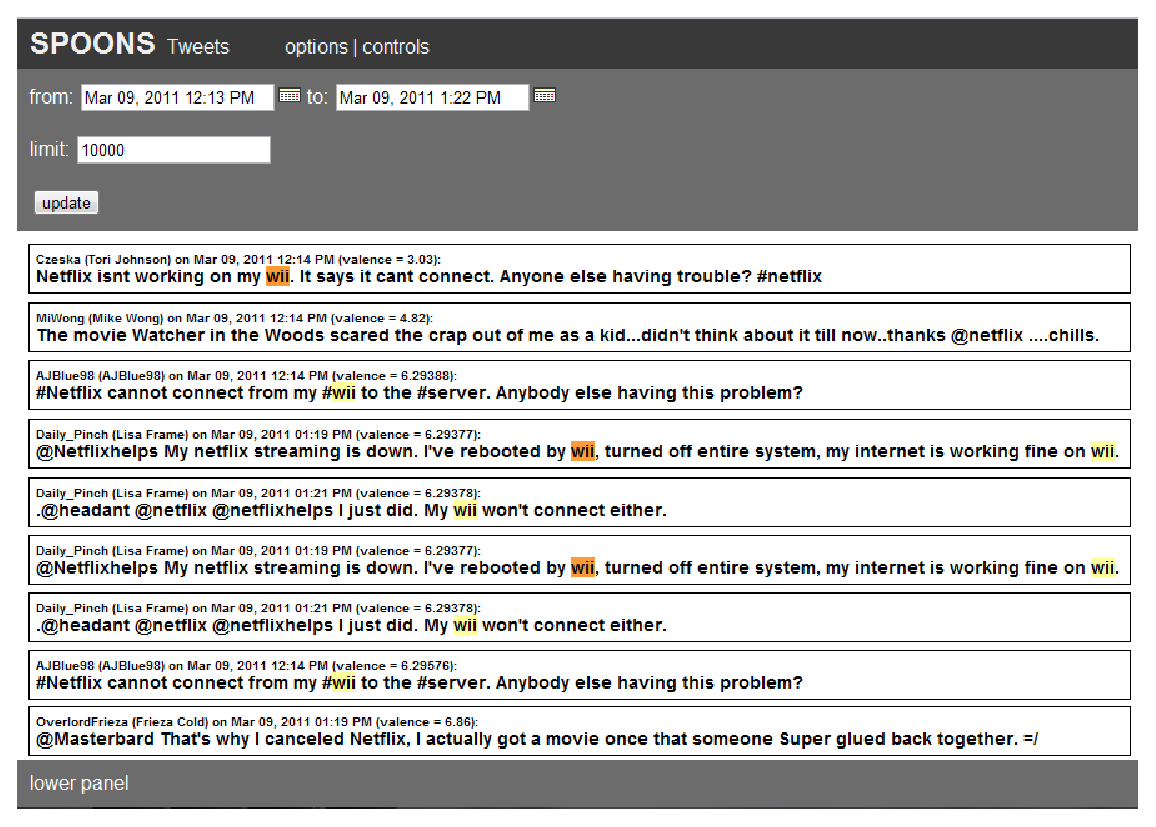
\includegraphics[width=140mm]{images/tweetexample.eps}
      \captionfonts
      \caption[Outage Tweets Example]{Tweets posted on March 9, 2011 during a disruption of Netflix
                                       streaming to the Nintendo Wii console.}
      \label{fig:tweetEx}
   \end{center}
\end{figure}


\chapter{Solution Overview}
\label{overview}

SPOONS (Swift Perception Of Online Negative Situations) is a system that is
designed to use tweets to detect outages in Netflix content delivery systems.
At present, the system supports a wide variety of detection methods that use some combination of time
series analysis, classification, natural language processing, sentiment
analysis, and filtering.

\begin{figure}
   \begin{center}
      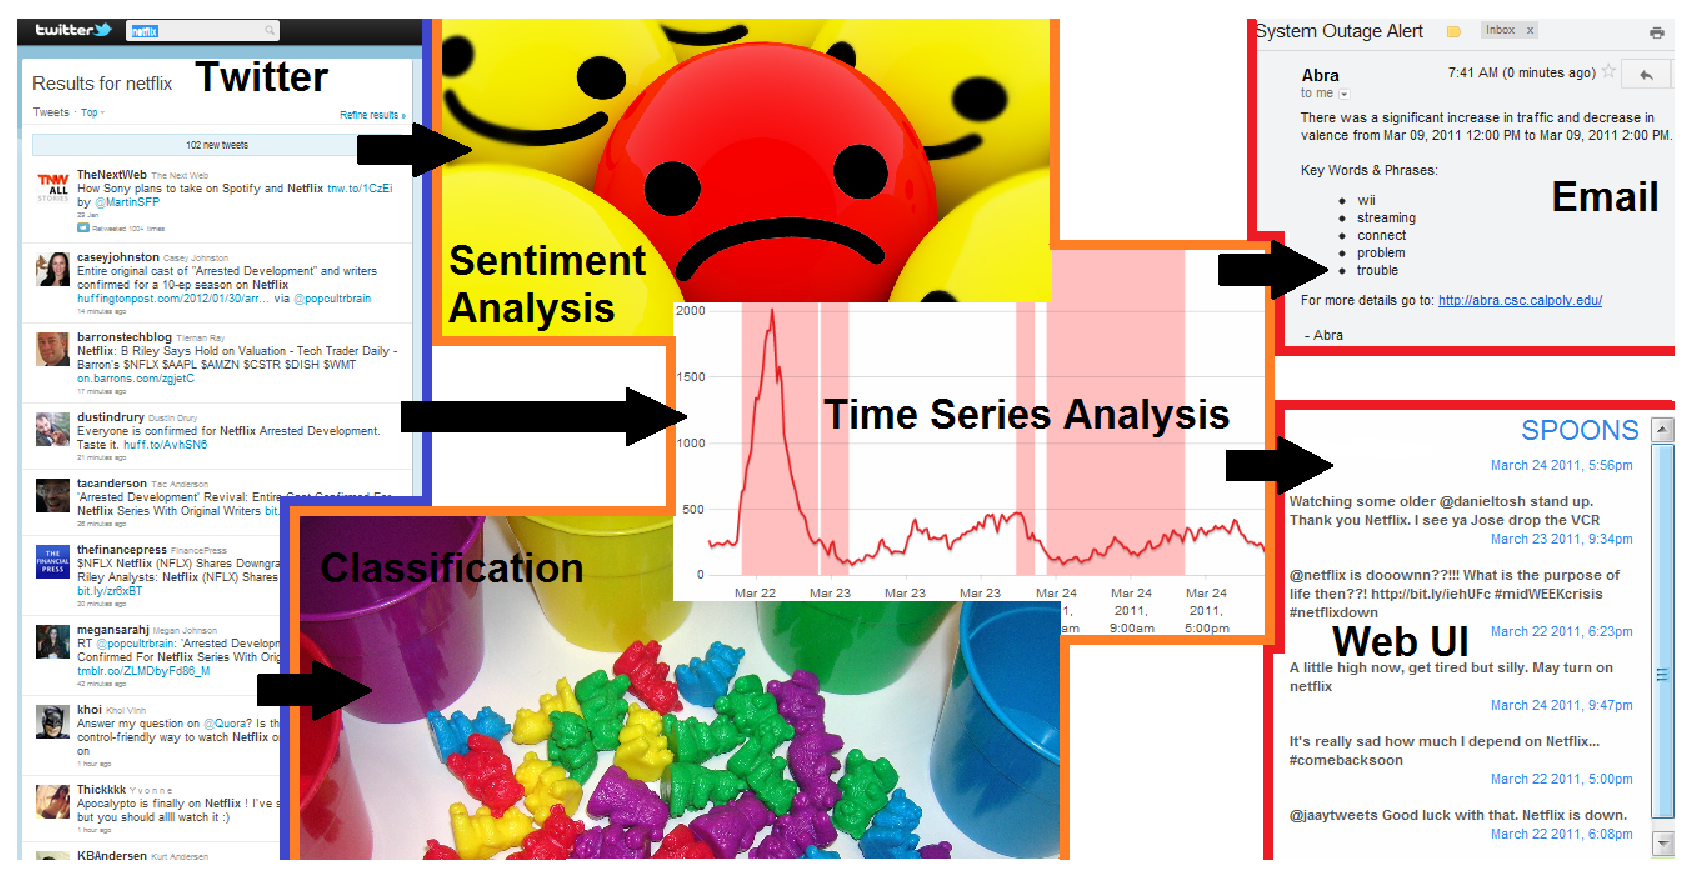
\includegraphics[width=140mm]{images/systemFlow.eps}
      \captionfonts
      \caption[System Concept Diagram]{This system concept diagram shows the general
                                       flow of processing done in the SPOONS system.}
      \label{fig:systemFlow}
   \end{center}
\end{figure}

Figure~\ref{fig:systemFlow} shows how the SPOONS system can be divided into three
main parts: {\color{blue}input}; {\color{orange}analysis methods}; and
{\color{red}output}. The inputs are tweets gathered from Twitter. Then the
analysis methods use a combination of sentiment estimation, classification, and
traffic volume analysis to detect when an outage is occurring.
The outputs of the system are: email alerts to Netflix engineers, and a web UI that displays
information about the outage.

\chapter{Ethics of Twitter Observation}

The work in this project uses content that users post on Twitter without their
knowledge. This monitoring system isn't being announced to the
public because widespread knowledge of it would increase the likelihood of a
malicious attack. This practice may lead to concerns about the level of privacy
or ownership being provided to Twitter users regarding the content they post
through the Twitter services. The goal of this section is to address these
concerns by providing more information about the Twitter services and how the
SPOONS system and this work uses the tweets.

\section{Twitter Terms of Service}

According to Twitter Terms of Service\cite{termsOfService} agreement that
everyone accepts automatically by accessing or using Twitter services:

\emph{``You retain your rights to any Content you submit, post or
display on or through the Services. By submitting, posting or displaying Content
on or through the Services, you grant us a worldwide, non-exclusive,
royalty-free license (with the right to sublicense) to use, copy, reproduce,
process, adapt, modify, publish, transmit, display and distribute such Content
in any and all media or distribution methods (now known or later developed).''}

\emph{``This license is you authorizing us to make your Tweets available to the
rest of the world and to let others do the same.''}

\emph{``You agree that this license includes the right for Twitter to make such
Content available to other companies, organizations or individuals who partner with
Twitter for the syndication, broadcast, distribution or publication of such
Content on other media and services, subject to our terms and conditions for
such Content use.''}

\emph{``We encourage and permit broad reuse of Content. The Twitter API exists to
enable this.''}

\emph{``Such additional uses by Twitter, or other companies, organizations or
individuals who partner with Twitter, may be made with no compensation paid to
you with respect to the Content that you submit, post, transmit or otherwise
make available through the Services.''}

In short, Twitter takes ownership of user tweets as soon as they are posted on Twitter.
Using the Twitter API allows SPOONS to obtain the tweets with the consent of Twitter.
Therefore, the collection and analysis of Twitter data by SPOONS is well withing the
Twitter Terms of Service.

\chapter{SPOONS Requirements}
Netflix has provided the following set of key requirements to be met by the
SPOONS system:

\paragraph{Structural Independence.}
The outage detection system shall be structurally independent of both the
software and the hardware infrastructure used by Netflix. It shall rely only on
information that is publicly available and free for use. This ensures that the
outage detection system stays up even when any or all Netflix servers are
experiencing downtime.

\paragraph{Use of Amazon Web Services.}
Netflix is one of the largest customers of Amazon.com's cloud computing
service, Amazon Web Services (AWS). AWS allows users to create new cloud
machines (instances) in many regions throughout the world. The outage
detection system shall be deployed on one or more AWS servers that are
operationally independent of other AWS servers used by Netflix. Using a cloud
solution allows the outage detection and alert system to be deployable on a
global scale.

\paragraph{Real-Time.}
Netflix's streaming services run in real-time and any downtime has an immediate
impact on customers. To minimize that impact, the outage detection system shall notify
Netflix of detected outages as soon as possible.

\paragraph{Precise Outage Detection.}
The number of non-outage situations that raise an alert shall be minimized.
While a small number of false positives detected in real-time may be acceptable,
the outage detection system shall detect outages and generate alerts with as
high precision as possible.

\paragraph{Comprehensive Outage Detection.}
Not all Netflix outages will generate a signal on Twitter. Those that don't may
be allowed to go unnoticed by the outage detection system (as the system will
have no basis for detecting them), but any outage that causes a signal on
Twitter shall be detected.

\paragraph{User-Friendly Online UI.}
The outage detection and alert system shall have an easy-to-use, informative,
online UI which shall provide Netflix employees with real-time information and
historic data about the state of Netflix according to Twitter. The information
provided shall include:

\begin{itemize}
   \item times of outages;
   \item times of other anomalous events;
   \item current and recent Netflix-related Twitter traffic trends;
   \item and samples of Netflix-related tweets.
\end{itemize}

\chapter{Contributions and Organization}
\label{contributions-organization}

SPOONS is a continual team effort and has been touched and improved by many different people.
The idea originated at Netflix and was passed to the ABRA team at Cal Poly. The ABRA team has published a paper
on SPOONS \cite{abraPaper}. In addition, Cailin Cushing defended a thesis using SPOONS\cite{cailinThesis}.

The main contributions of this work are the design and implementation of the SPOONS system, framework, server architecture,
distribution model, and database schema. As well as the design and implementation of classification based outage detection
methods.

The rest of the paper is organized as follows. Chapter~\ref{background-related-work} covers background and related work.
Chapter~\ref{arch} discusses the architecture of SPOONS. Chapter~\ref{classifiers} discuss the details of the classifiers
used in SPOONS. Chapters~\ref{outage-detection} extends the problem of classification to full outage detection. Chapter~\ref{conclusions} wraps up the paper.

\part{Background \& Related Work}
\label{background-related-work}

%\chapter{Text Stream Analysis}
%\label{background-text-stream}
%Text Stream Analysis \cite{Bansal}\cite{Grinev}\cite{Huang}.

\chapter{Twitter Classification}
\label{background-classification}
There has been much work in using classifiers on both tweets and Twitter users.
Most of the classification effort has gone into trying to determine the sentiment,
the general feeling, of a tweet \cite{Jiang}\cite{Mukherjee}\cite{Saif}\cite{Wang}.
Raz et al. tackle the task of classifying humorous tweets as a specific type of humor
such as irony, observational, or wordplay\cite{Raz}.
The traditional text classification task of topic modeling has also been attempted various times\cite{hong}\cite{Zhao}.
Instead of trying to classify tweets, Pennacchiotti et al. try to classify a user associations from
their tweets\cite{Pennacchiotti}.

The common theme in all of these classification attempts is that tweets are much more difficult to
classify than more traditional media sources, eg. news articles, because of their length and language.
The 140 character limit on tweets severely limits the information content of a tweet.
Partially because of the character limit, slang and informal language are commonplace in tweets.

\chapter{Classifiers}
\label{background-classification-classifiers}
SPOONS uses a variety of different classifiers for text classification.
This section gives an overview of each different type of classifier used.

\section{Naive Bayes}
\label{background-classification-classifiers-naive-bayes}
Naive Bayes classifier work by applying the Bayes' theorem with the assumption that
the probability of each feature in a document is independent from the probability of
any other feature appearing in the same document.\cite{Kibriya}\cite{Frank}

Let $c$ be a specific class in the set of possible classes $C$.
Let $d$ be a document composed of a vector of $n$ features, $d = (\textrm{f}_{1}, \textrm{f}_{2}, ..., \textrm{f}_{n})$.
The Bayes' theorem states that the probability of observing class $c$ given document $d$
can be represented as:

\begin{equation}
   Pr(c|d) = \frac{Pr(c) \cdot Pr(d|c)}{Pr(d)}
\end{equation}

$Pr(c)$ is the \textsf{prior probability} of class $c$. That is, the probability of
observing $c$ regardless of the document attached to it. When training the classifier, this
is just the percentage of times that the class appeared in the training set.

$Pr(d)$ is the \textsf{prior probability} of document $d$. Like $Pr(c)$, it is just the
probability of observing the collection of features $d$ regardless of the class associated with it.
Note that for classification, it may not be necessary to compute $Pr(d)$ because it is constant among all
documents and classes. A classifier can just choose the class with the largest $Pr(c) \cdot Pr(d|c$ term.

$Pr(d|c)$ is the probability of observing document $d$ given that $d$ is already recognized as belonging to
class $c$. Remember that document $d$ is really just a vector of $n$ features, $(\textrm{f}_{1}, \textrm{f}_{2}, ..., \textrm{f}_{n})$.
Assuming \textbf{conditional independence} (the \textsf{naive} part in Naive Bayes), $Pr(d|c)$ can be
constructed as a product of the probability of observing each feature in $d$:

\begin{equation}
   Pr(d|c) = Pr(\textrm{f}_{1}|c) \cdot Pr(\textrm{f}_{2}|c) \cdot ... \cdot Pr(\textrm{f}_{n}|c) = \prod_{i = 1}^{n}Pr(\textrm{f}_{i}|c)
\end{equation}

Now the last step is to estimate the conditional probabilities of the $n$ features.
When dealing with discrete features, then estimating $Pr(\textrm{f}_{m}|c)$ ($1 \leq m \leq n$) can be done by
finding the percentage of training documents that contain feature $\textrm{f}_{m}$ and have class $c$.

\section{Bayes Net}
\label{background-classification-classifiers-bayes-net}
A Bayesian Networks are probabilistic, directed acyclic graphs that represents a set of random variables and their conditional probabilities.
In a Bayesian Network, each edge represents the conditional probability between two nodes. Each node represents a variable and a probability
function that takes as input the state of the node's parents.\cite{Pearl}\cite{Neapolitan}

Figure~\ref{fig:bayesNet1} shows a simple Bayesian Network that models the chance of going on a picnic.
Note that the whether or not it is Spring affects the chance of it raining; and both the season and weather
affect the chance of going on a picnic.

Figure~\ref{fig:bayesNet2} shows the probability functions for the network. The chance of the season being Spring if
fully independent, and therefore takes no parameters into its probability function. However, the weather and picnic decision
takes one and two input parameters respectively.

\begin{figure}
   \begin{center}
      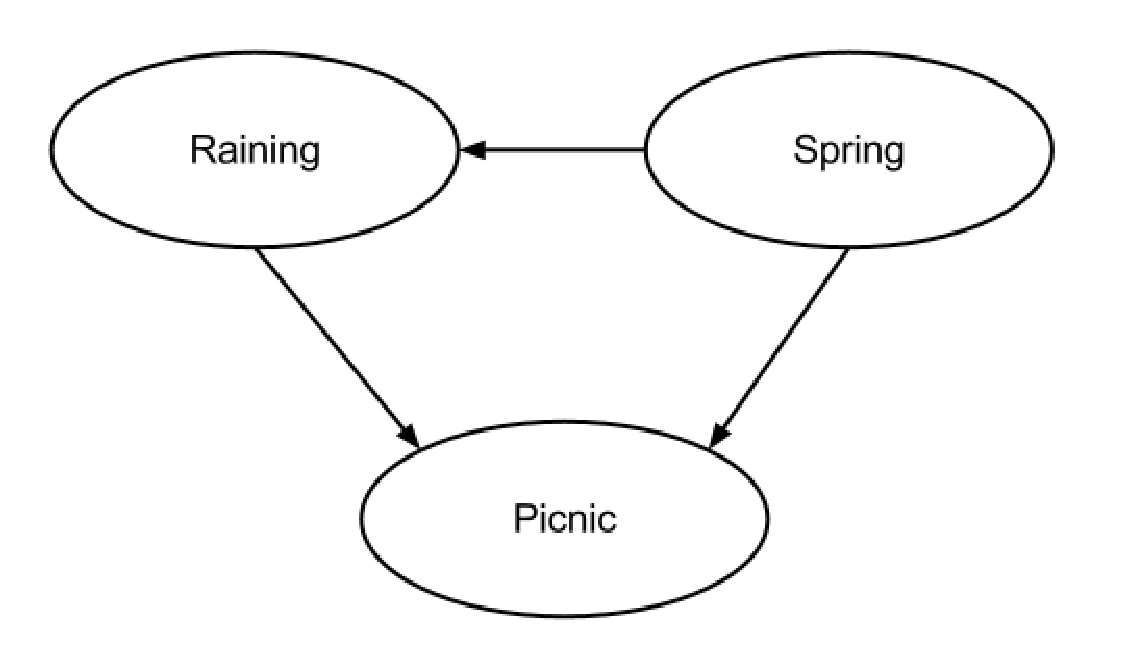
\includegraphics[width=0.4\textwidth]{images/Bayes_Net_1.eps}
      \captionfonts
      \caption[Simple Bayes Net]{A simple Bayesian Network modeling the chance of going on a picnic given the season and weather. The season affects the weather and both the season and weather affect the chance of going on a picnic.}
      \label{fig:bayesNet1}
   \end{center}
\end{figure}

\begin{figure}
   \begin{center}
      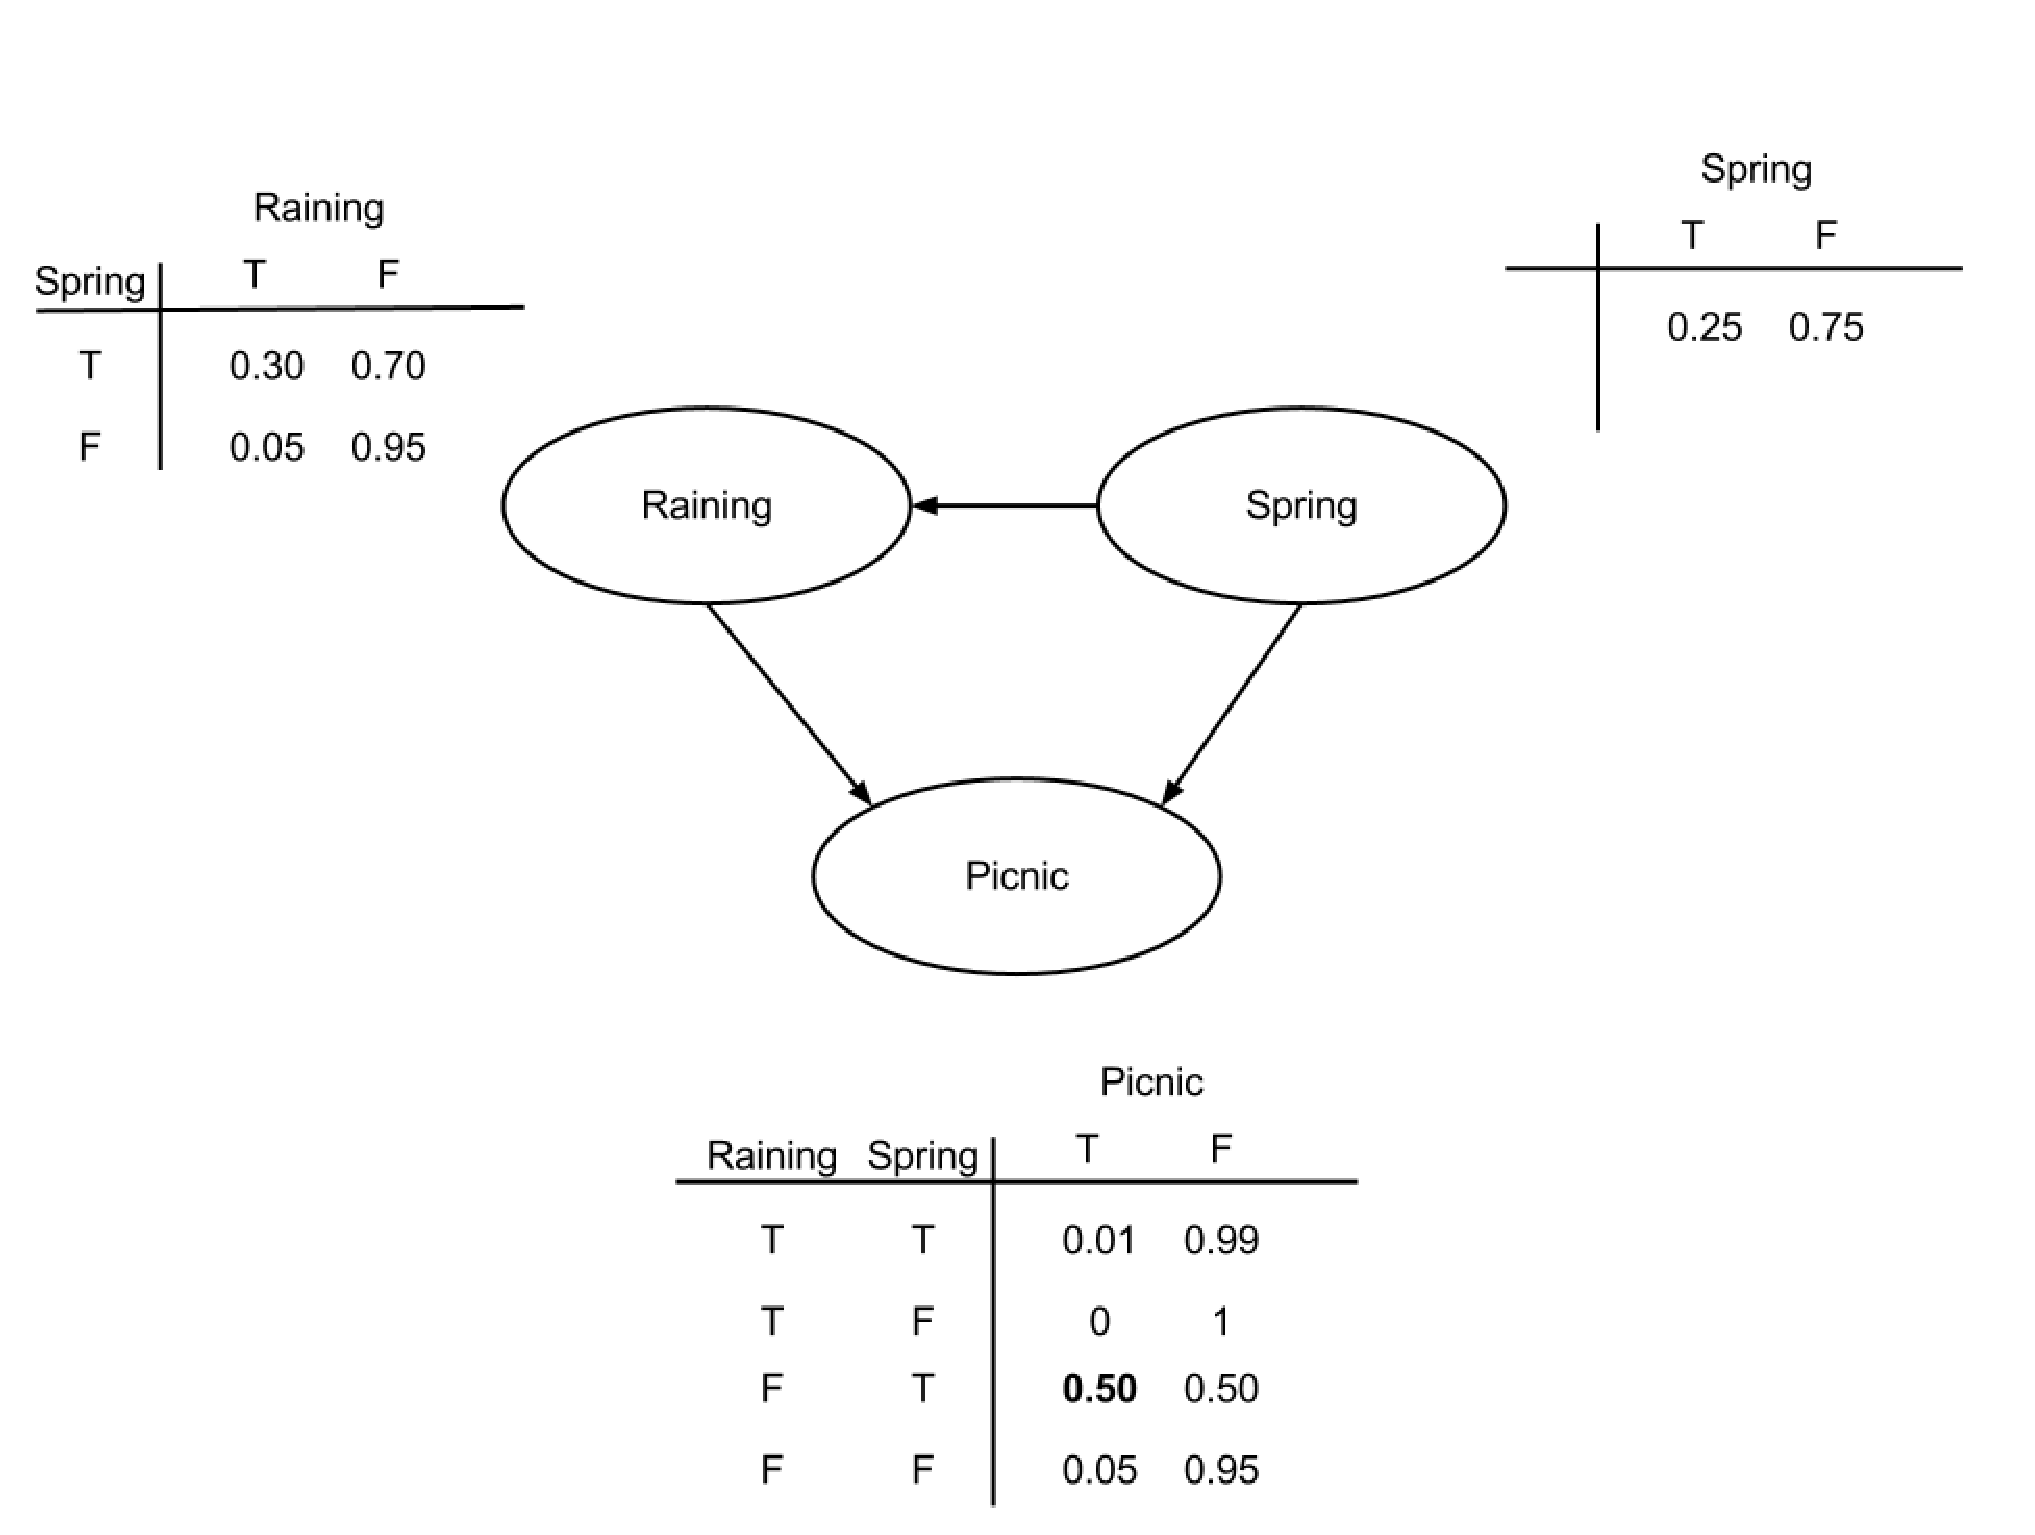
\includegraphics[width=0.8\textwidth]{images/Bayes_Net_2.eps}
      \captionfonts
      \caption[Bayes Net With Probabilities]{The simple Bayesian Network augmented with the probability functions for each node.}
      \label{fig:bayesNet2}
   \end{center}
\end{figure}

\section{J48}
\label{background-classification-classifiers-j48}
J48 is a specific implementation of the C4.5 algorithm.
C4.5 is an algorithm that is used to generate a decision tree given a training set.

\subsection{Decision Trees}
\label{background-classification-classifiers-j48-decision-trees}
A decision tree is a simple data structure used to come to come conclusion based off of a number of observations.
At each non-terminal node, a question is asked. The answers to the question are represented by the node's outgoing edges.
The tree is traversed in this fashion until a terminal node is reached. The terminal node contains the final conclusion.
In a classification context, each non-terminal node is labeled with an attribute, each edge is the value (or range of values)
for that attribute, and each terminal node is a class. Each attribute can only appear once in the tree.

\begin{figure}
   \begin{center}
      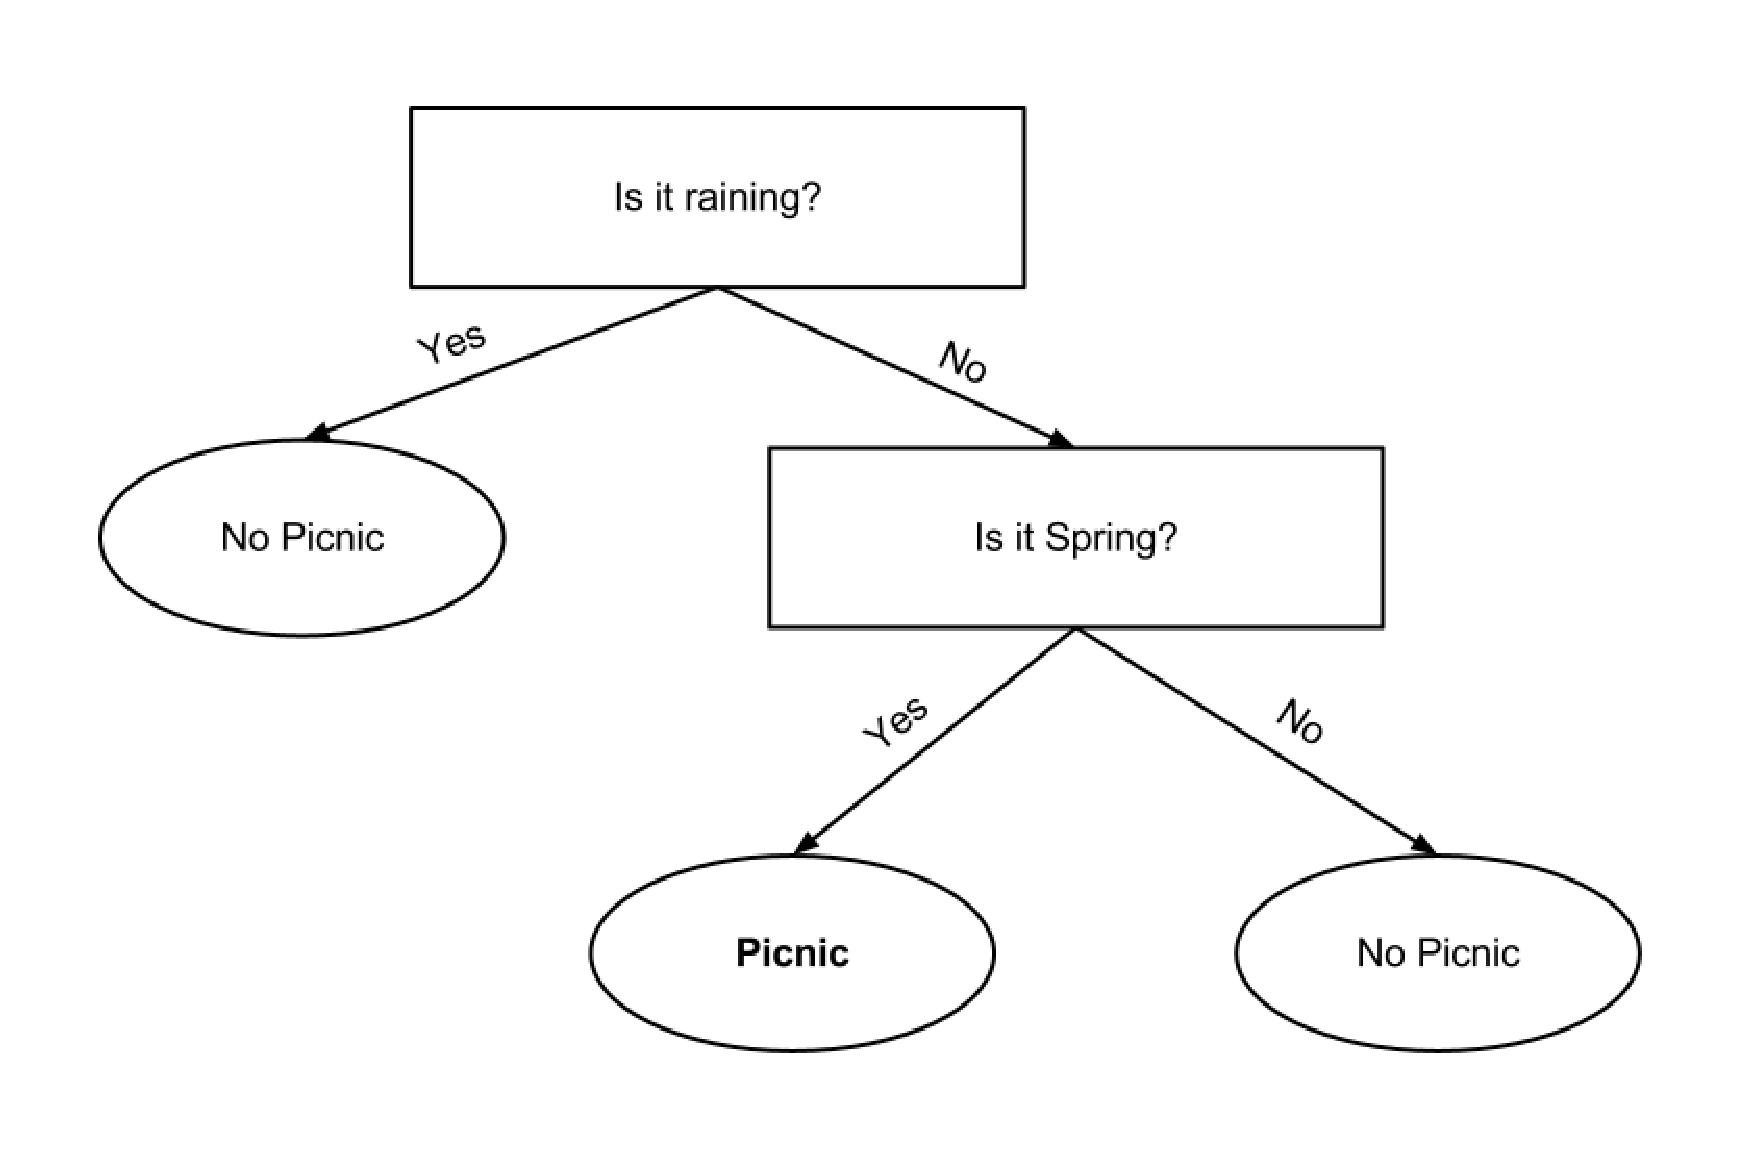
\includegraphics[width=0.8\textwidth]{images/Decision_Tree.eps}
      \captionfonts
      \caption[Simple Decision Tree]{A simple decision tree trying to answer the question of whether or not to go on a picnic.}
      \label{fig:decisionTree}
   \end{center}
\end{figure}

Figure~\ref{fig:decisionTree} shows a decision tree that may be generated for the picnic example discussed in Section~\ref{background-classification-classifiers-bayes-net}.
Note that once the decision tree is built, reaching a terminal node is fairly trivial.

\subsection{C4.5}
\label{background-classification-classifiers-j48-c45}
C4.5 will recursively build a decision tree by continually splitting the dataset on a single attribute\cite{Quinlan}.
The splitting attribute is determined by the normalized information gain (Kullback-Leibler divergence) and becomes a
node in the tree and the possible values for the attribute become edges. Each subtree is then recursively built using only the
data where the splitting attribute takes the value given by the incoming edge. The algorithm has two stopping conditions.
First, when all the data has the same class. In which case a single node tree will be constructed that contains the class.
Secondly, when there are no more attributes or when the information gain from splitting on each attribute is below a threshold.
In this case, a single node tree will be constructed which contains the plurality class.

\section{K-Nearest Neighbors}
\label{background-classification-classifiers-knn}
$k$-Nearest Neighbors (KNN) is simple and effective classification technique\cite{Duda}.
While training, the classifier remembers the entire training set.
During the classification phase, the classifier will find the $k$ nearest neighbors
to the query point. The predicted class is simply the plurality of the $k$ nearest neighbors.
Figure~\ref{fig:knn} shows an example of $k$-Nearest Neighbors with a simple search space.

\begin{figure}
   \begin{center}
      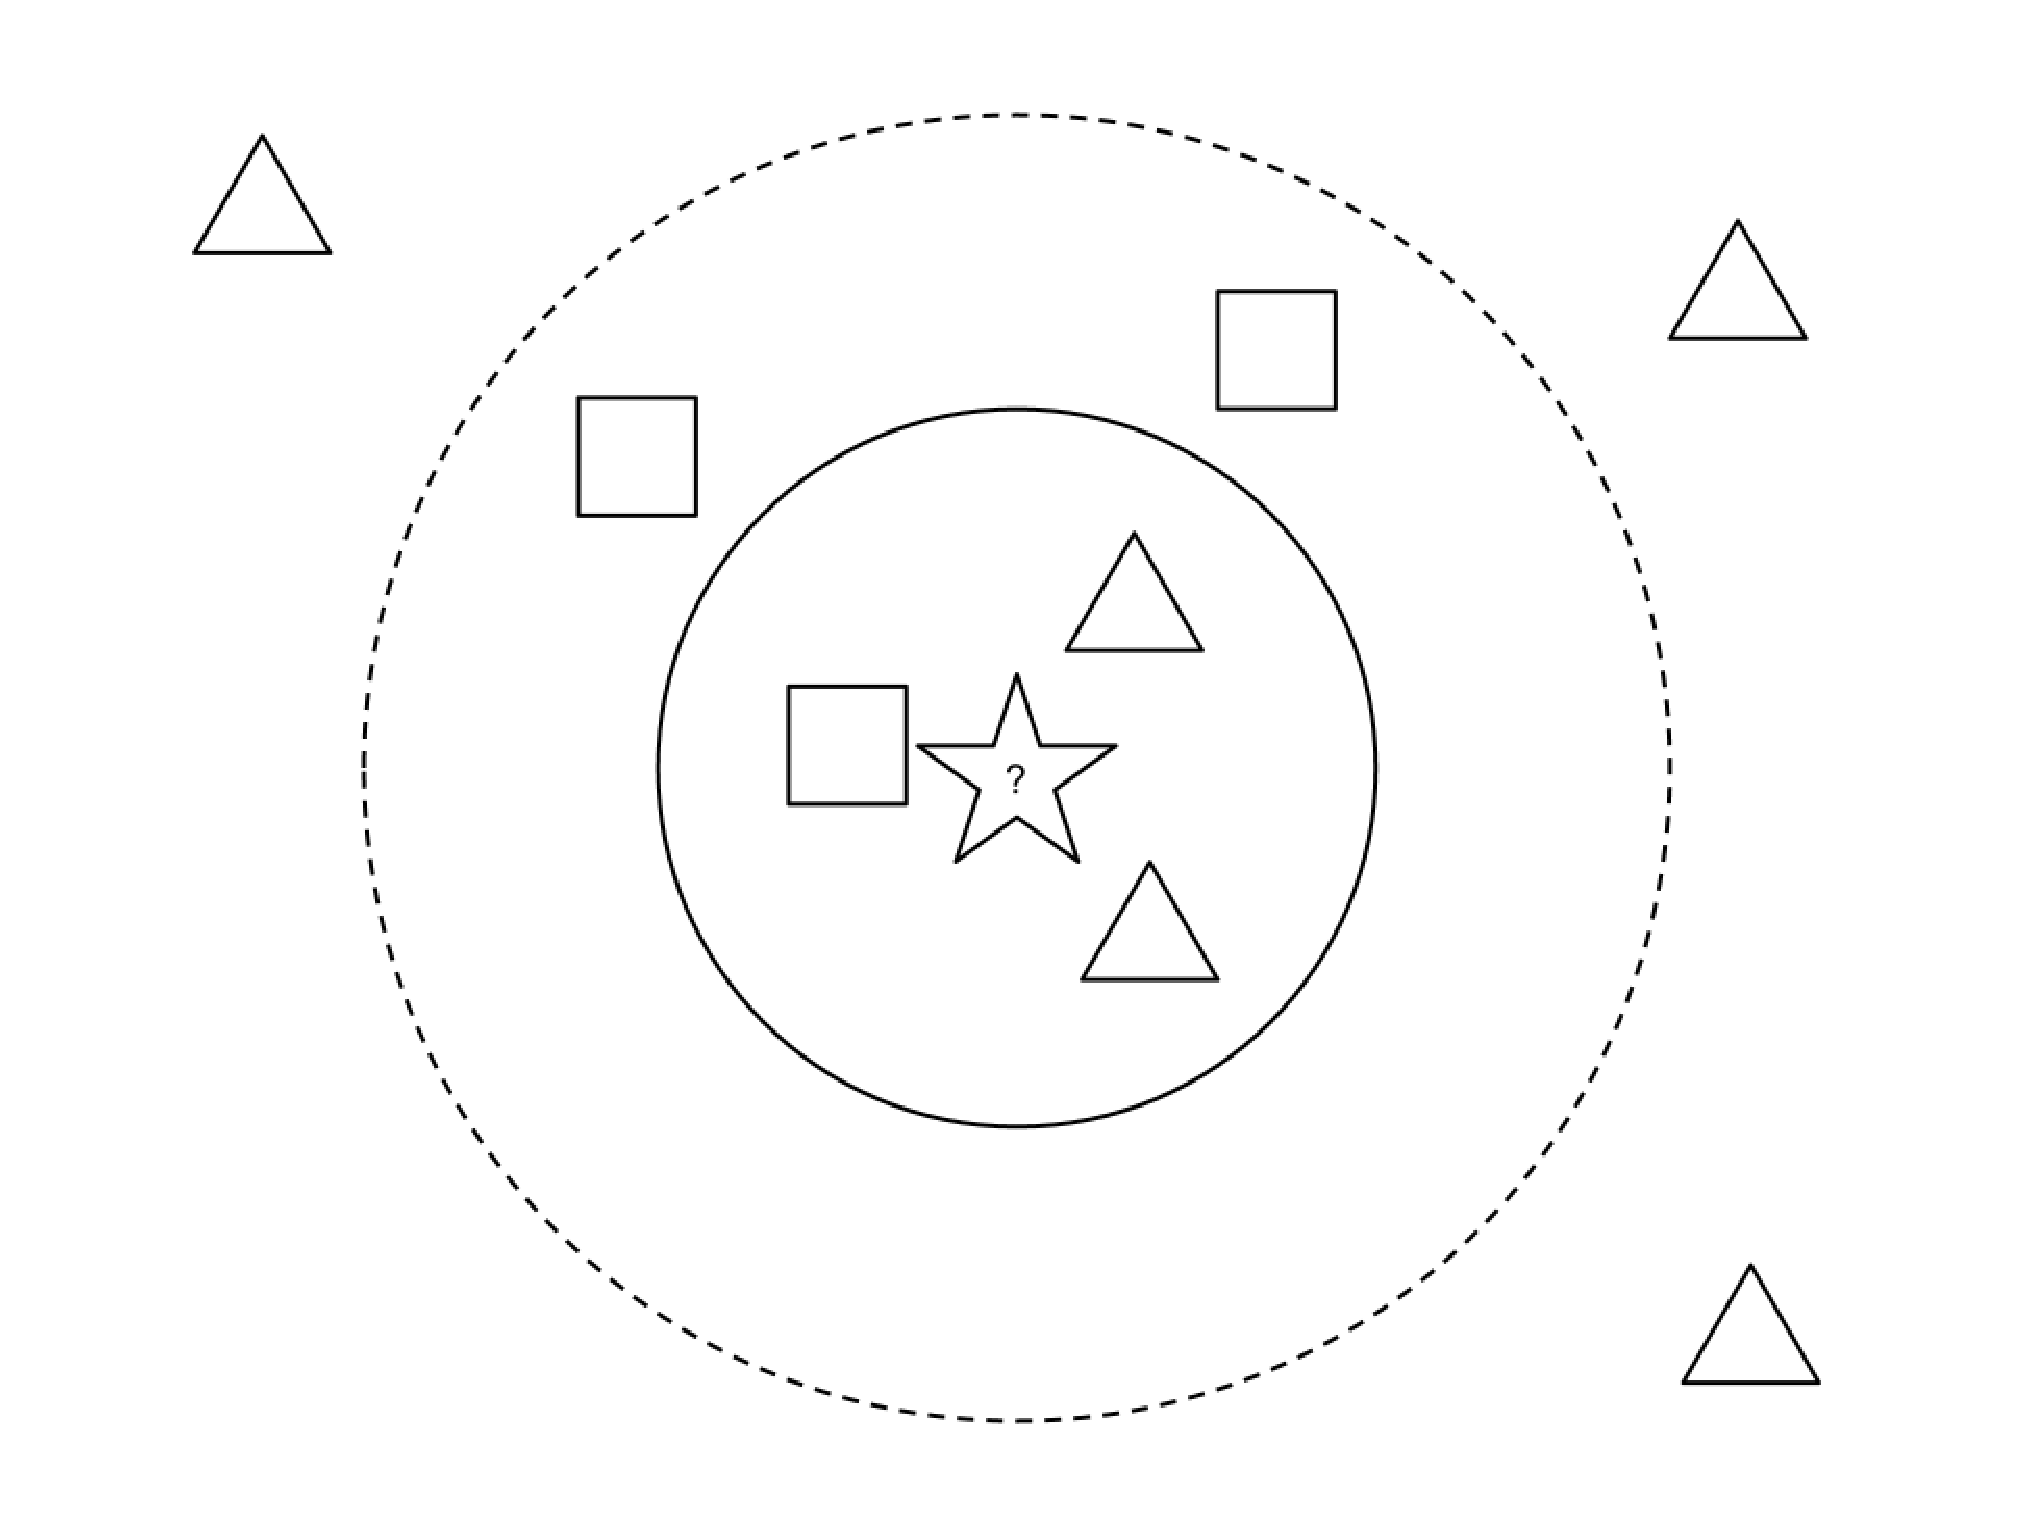
\includegraphics[width=0.4\textwidth]{images/KNN.eps}
      \captionfonts
      \caption[K-Nearest Neighbors]{A simple example of KNN. If $k = 3$, then the query point (the star) will be classified as a triangle. However, if $k = 5$ then the query point will be classified as a square.}
      \label{fig:knn}
   \end{center}
\end{figure}

\section{Support Vector Machines}
\label{background-classification-classifiers-svm}
Support Vector Machines (SVMs) are considered one of the best off-the-shelf classification techniques\cite{Vapnik}.
When training, SVMs use hyperplanes to partition the data into surfaces based off of the different classes of the training examples.
When classifying, the SVM will find which surface the query point falls on and give that class to the point.
SVMs will try and choose the partitioning hyperplane to maximize the margin between the two groups of data.
Depending on the implementation, the SVM may choose the optimal partition or just an approximation.

\begin{figure}
   \begin{center}
      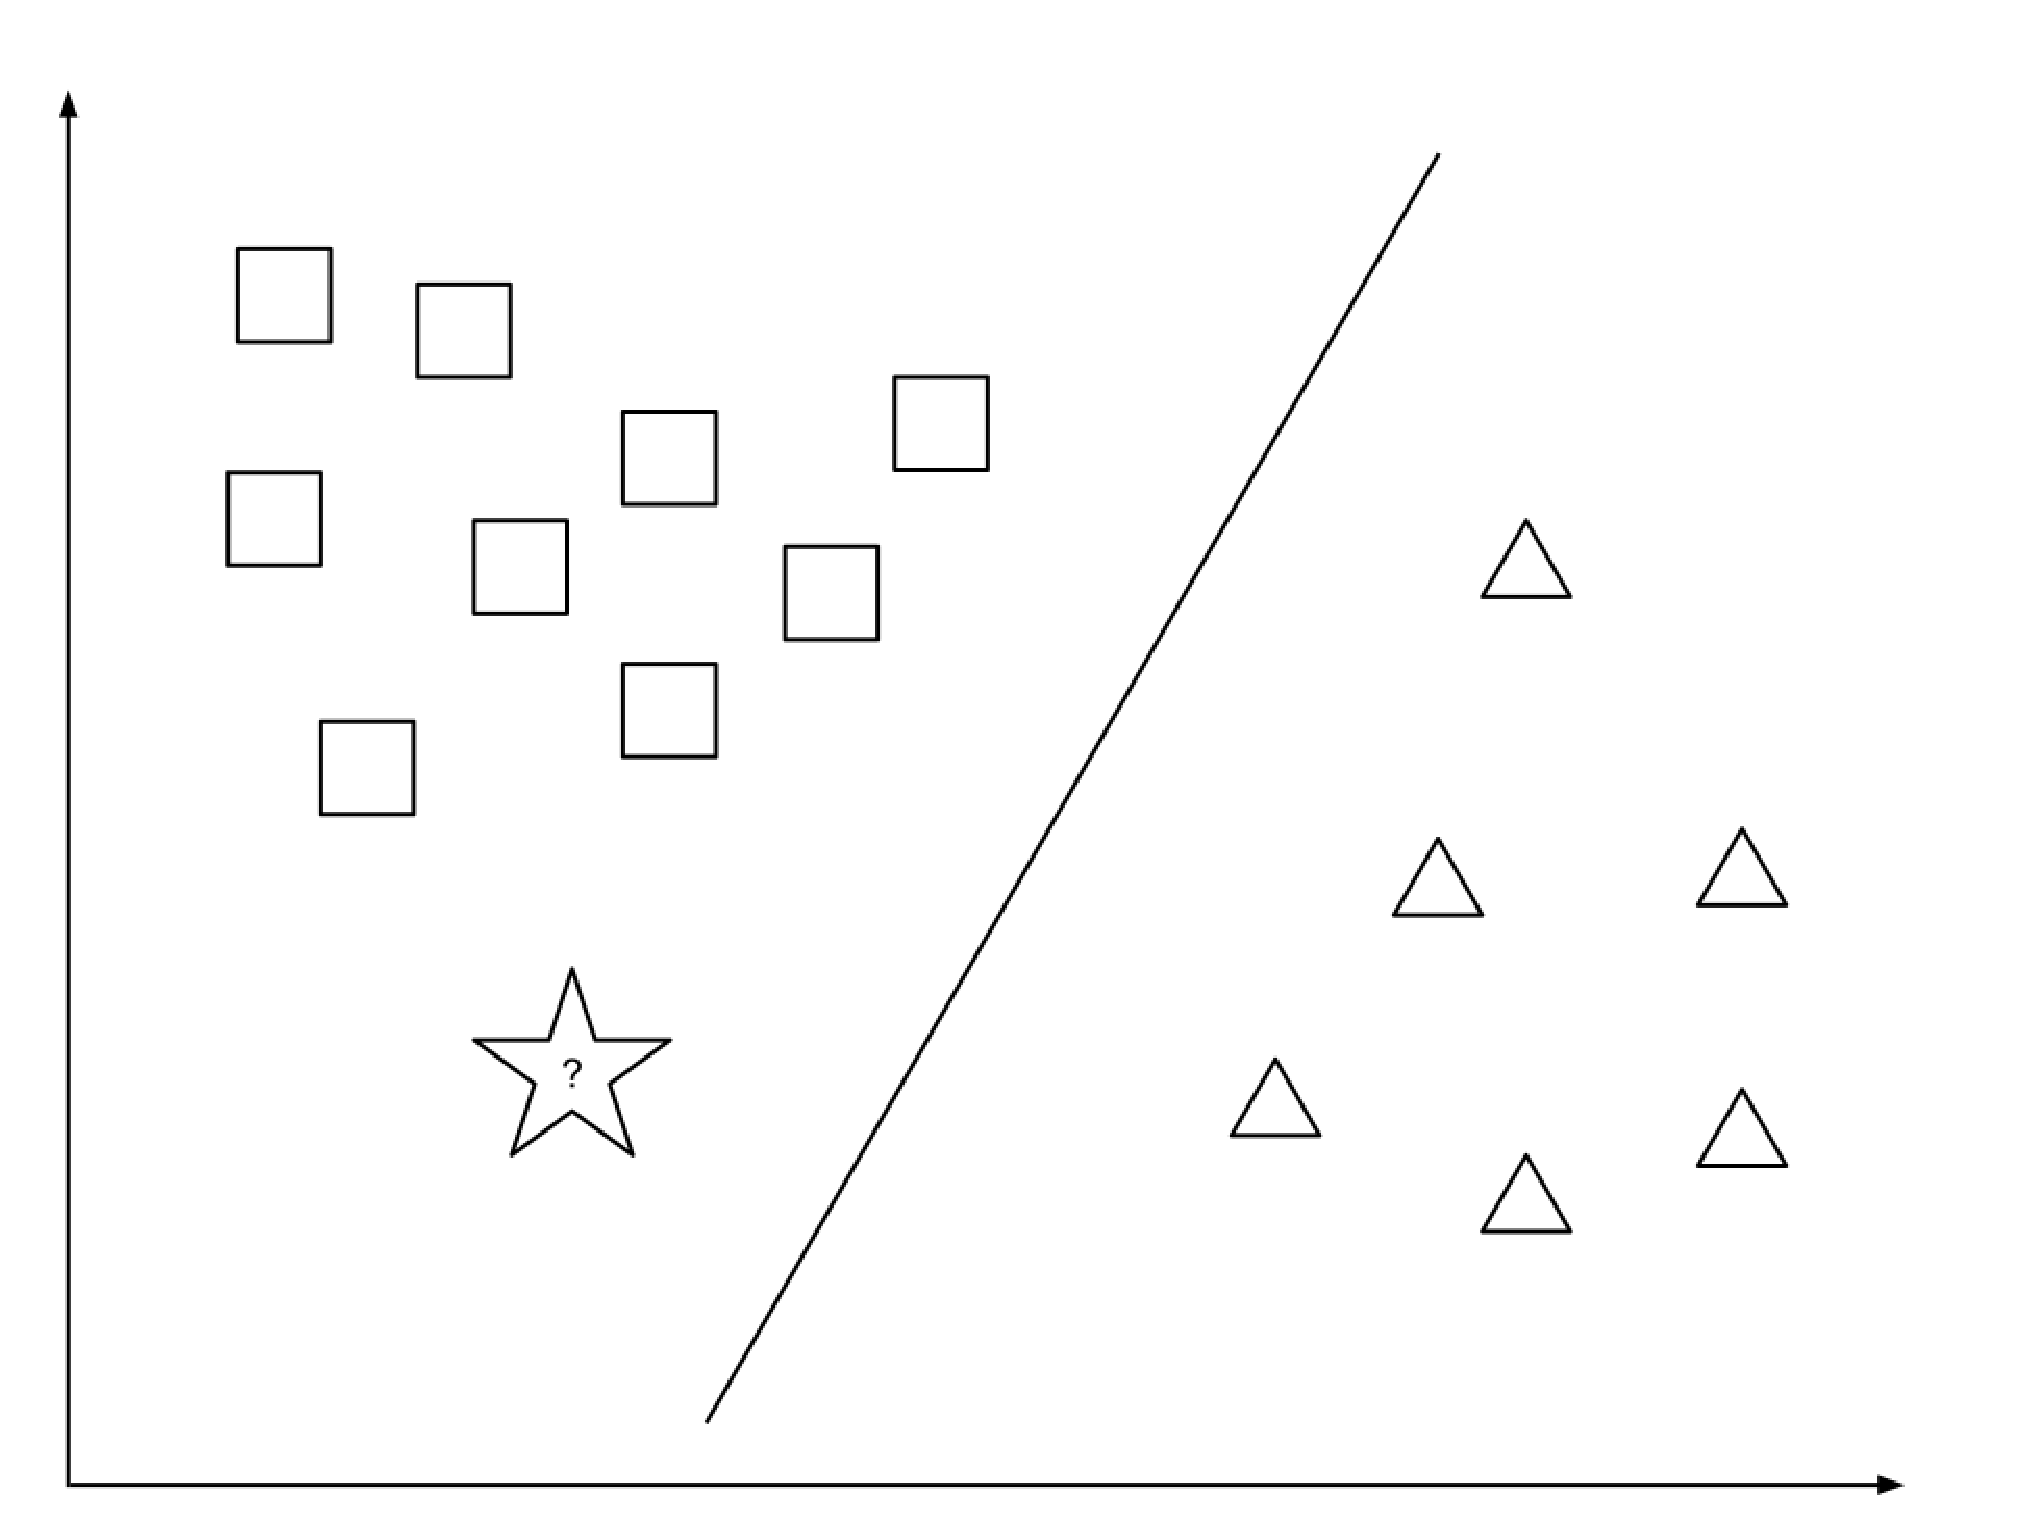
\includegraphics[width=0.4\textwidth]{images/SVM.eps}
      \captionfonts
      \caption[Support Vector Machine]{A simple example of a support vector machine. The SVM chose a partition that maximizes the margin between the squares and triangles.}
      \label{fig:svm}
   \end{center}
\end{figure}

Figure~\ref{fig:svm} shows a simple example of a linear binary SVM.
Note that the partition line is chosen to maximize the distance between the triangles and squares.
The query point (the star) falls into the squares' partition and is therefore classified as a square.

\subsection{Sequential Minimal Optimization}
\label{background-classification-classifiers-svm-smo}
Sequential Minimal Optimization (SMO) is an efficient algorithm for solving SVMs invented by John Platt in 1998\cite{Platt}.

\section{BPNB}
\label{background-classification-classifiers-bpnb}
BPNB is a method developed by Chu\cite{bpnb}.
It is based off of Naive Bayes, except the relative probability of each feature is accounted for.

Let $c$ be a specific class in the set of possible classes $C$.
Let $d$ be a document composed of a vector of $n$ features, $d = (\textrm{f}_{1}, \textrm{f}_{2}, ..., \textrm{f}_{n})$.
BPNB states that the probability of observing class $c$ given document $d$
can be represented as:

\begin{equation}
   Pr(c|d) = Pr(c) \cdot \prod_{i = 1}^{n}g(\textrm{f}_{i},c)
\end{equation}

Where $g(\textrm{f}_{m}, c)$ is the weight of feature $\textrm{f}_m$ in class $c$.

\begin{equation}
   g(\textrm{f}_m, c) = \beta^{1 - \frac{Pr(\textrm{f}_m|c)}{Ave(\textrm{f}_m)}}, 0 < \beta < 1
\end{equation}

\begin{equation}
   Ave(\textrm{f}_m) = \frac{\sum_{i=1}^{|C|} Pr(\textrm{f}_m|c_{i})}{|C|}, c_i \in C
\end{equation}

\section{WEKA}
\label{background-weka}
SPOONS utilizes several classifiers provided in the \textit{WEKA Machine Learning Package}.
WEKA is an open source package written under the GNU General Public License\cite{weka}.

\chapter{Twitter API}
\label{background-twitter-api}
All of the data data that SPOONS uses is obtained in real time using the Twitter Search REST API\cite{TwitterAPI}.

\section{Rate Limiting}
\label{api-rate-limit}
Twitter imposes a limit on the number of queries to the Search API. Twitter does not publish the official
limit. However, our experiments suggest that SPOONS can query the API for all new Tweets once every two minutes without
suffering from rate limiting.

\section{Pagination}
\label{api-pagination}
Twitter paginates the results from its search API. The maximum results you can get per page is 100, and each
query can return at most 15 pages. Therefore when there are more than 1500 tweets generated per minute,
SPOONS must do multiple search queries.

\section{Query Anatomy}
\label{api-anatomy}
The typical structure of a Twitter API query is shown in Figure~\ref{fig:apiQuery}.

\begin{figure}[H]
   \begin{center}
      \fbox{
         \begin{minipage}{12cm}
            \begin{center}
               http://search.twitter.com/search.\textbf{json}?\textbf{q}=$\langle$query$\rangle$\&\textbf{rpp}=100\&\\
               \textbf{result\_type}=recent\&\textbf{since\_id}=$\langle$tweet id$\rangle$\&\textbf{max\_id}=$\langle$tweet id$\rangle$
            \end{center}
         \end{minipage}
      }
      \captionfonts
      \caption[Twitter API Query]{The structure of a typical query to the Twitter API.}
      \label{fig:apiQuery}
   \end{center}
\end{figure}

The parameters are:

\begin{description}

\item[json:]
Twitter can supply the result data in either ATOM or JSON format. Testing with both have shown that the ATOM
results are less consistent and provide less data. Because of the more accurate information returned from the JSON
API, we are able to write more efficient queries. Using the ATOM API, we could query Twitter only once every five
minutes; as opposed to every two minutes with the JSON API.

\item[q:]
The search query. Twitter supports some advanced search features such as conjunction and negation.

\item[rpp:]
``Results Per Page''. Twitter paginates the responses from the Search API. SPOONS always uses the maximum pagination value to decrease the number of requests per hour and lessen the chance of being rate limited.

\item[result\_type:]
Twitter allows users to get results ordered by either relevance or time. Since we want to gather all tweets about
our query, we choose to get the results ordered by time. In addition, the ``since\_id'' and ``max\_id''
parameters do not work when results are sorted by relevance.

\item[since\_id:]
The id of the oldest tweet that should be returned. This is not a hard limit, but provides a nice starting point.

\item[max\_id:]
The id of the most recent tweet that should be returned. It may seem counter-intuitive to provide a cap on the
most recent tweet, when one wants to query for all of the most recent tweets. However when a query spans across
more than 15 pages, it will need to be broken into a new query restarting at the first page. In this situation,
not providing an upper limit will include new tweets outside of the original search scope. This can result in tweets
are forever lost to us.

\end{description}

\section{Result Anatomy}
\begin{figure}
   \begin{center}
      \fbox{
         \begin{minipage}{160mm}
            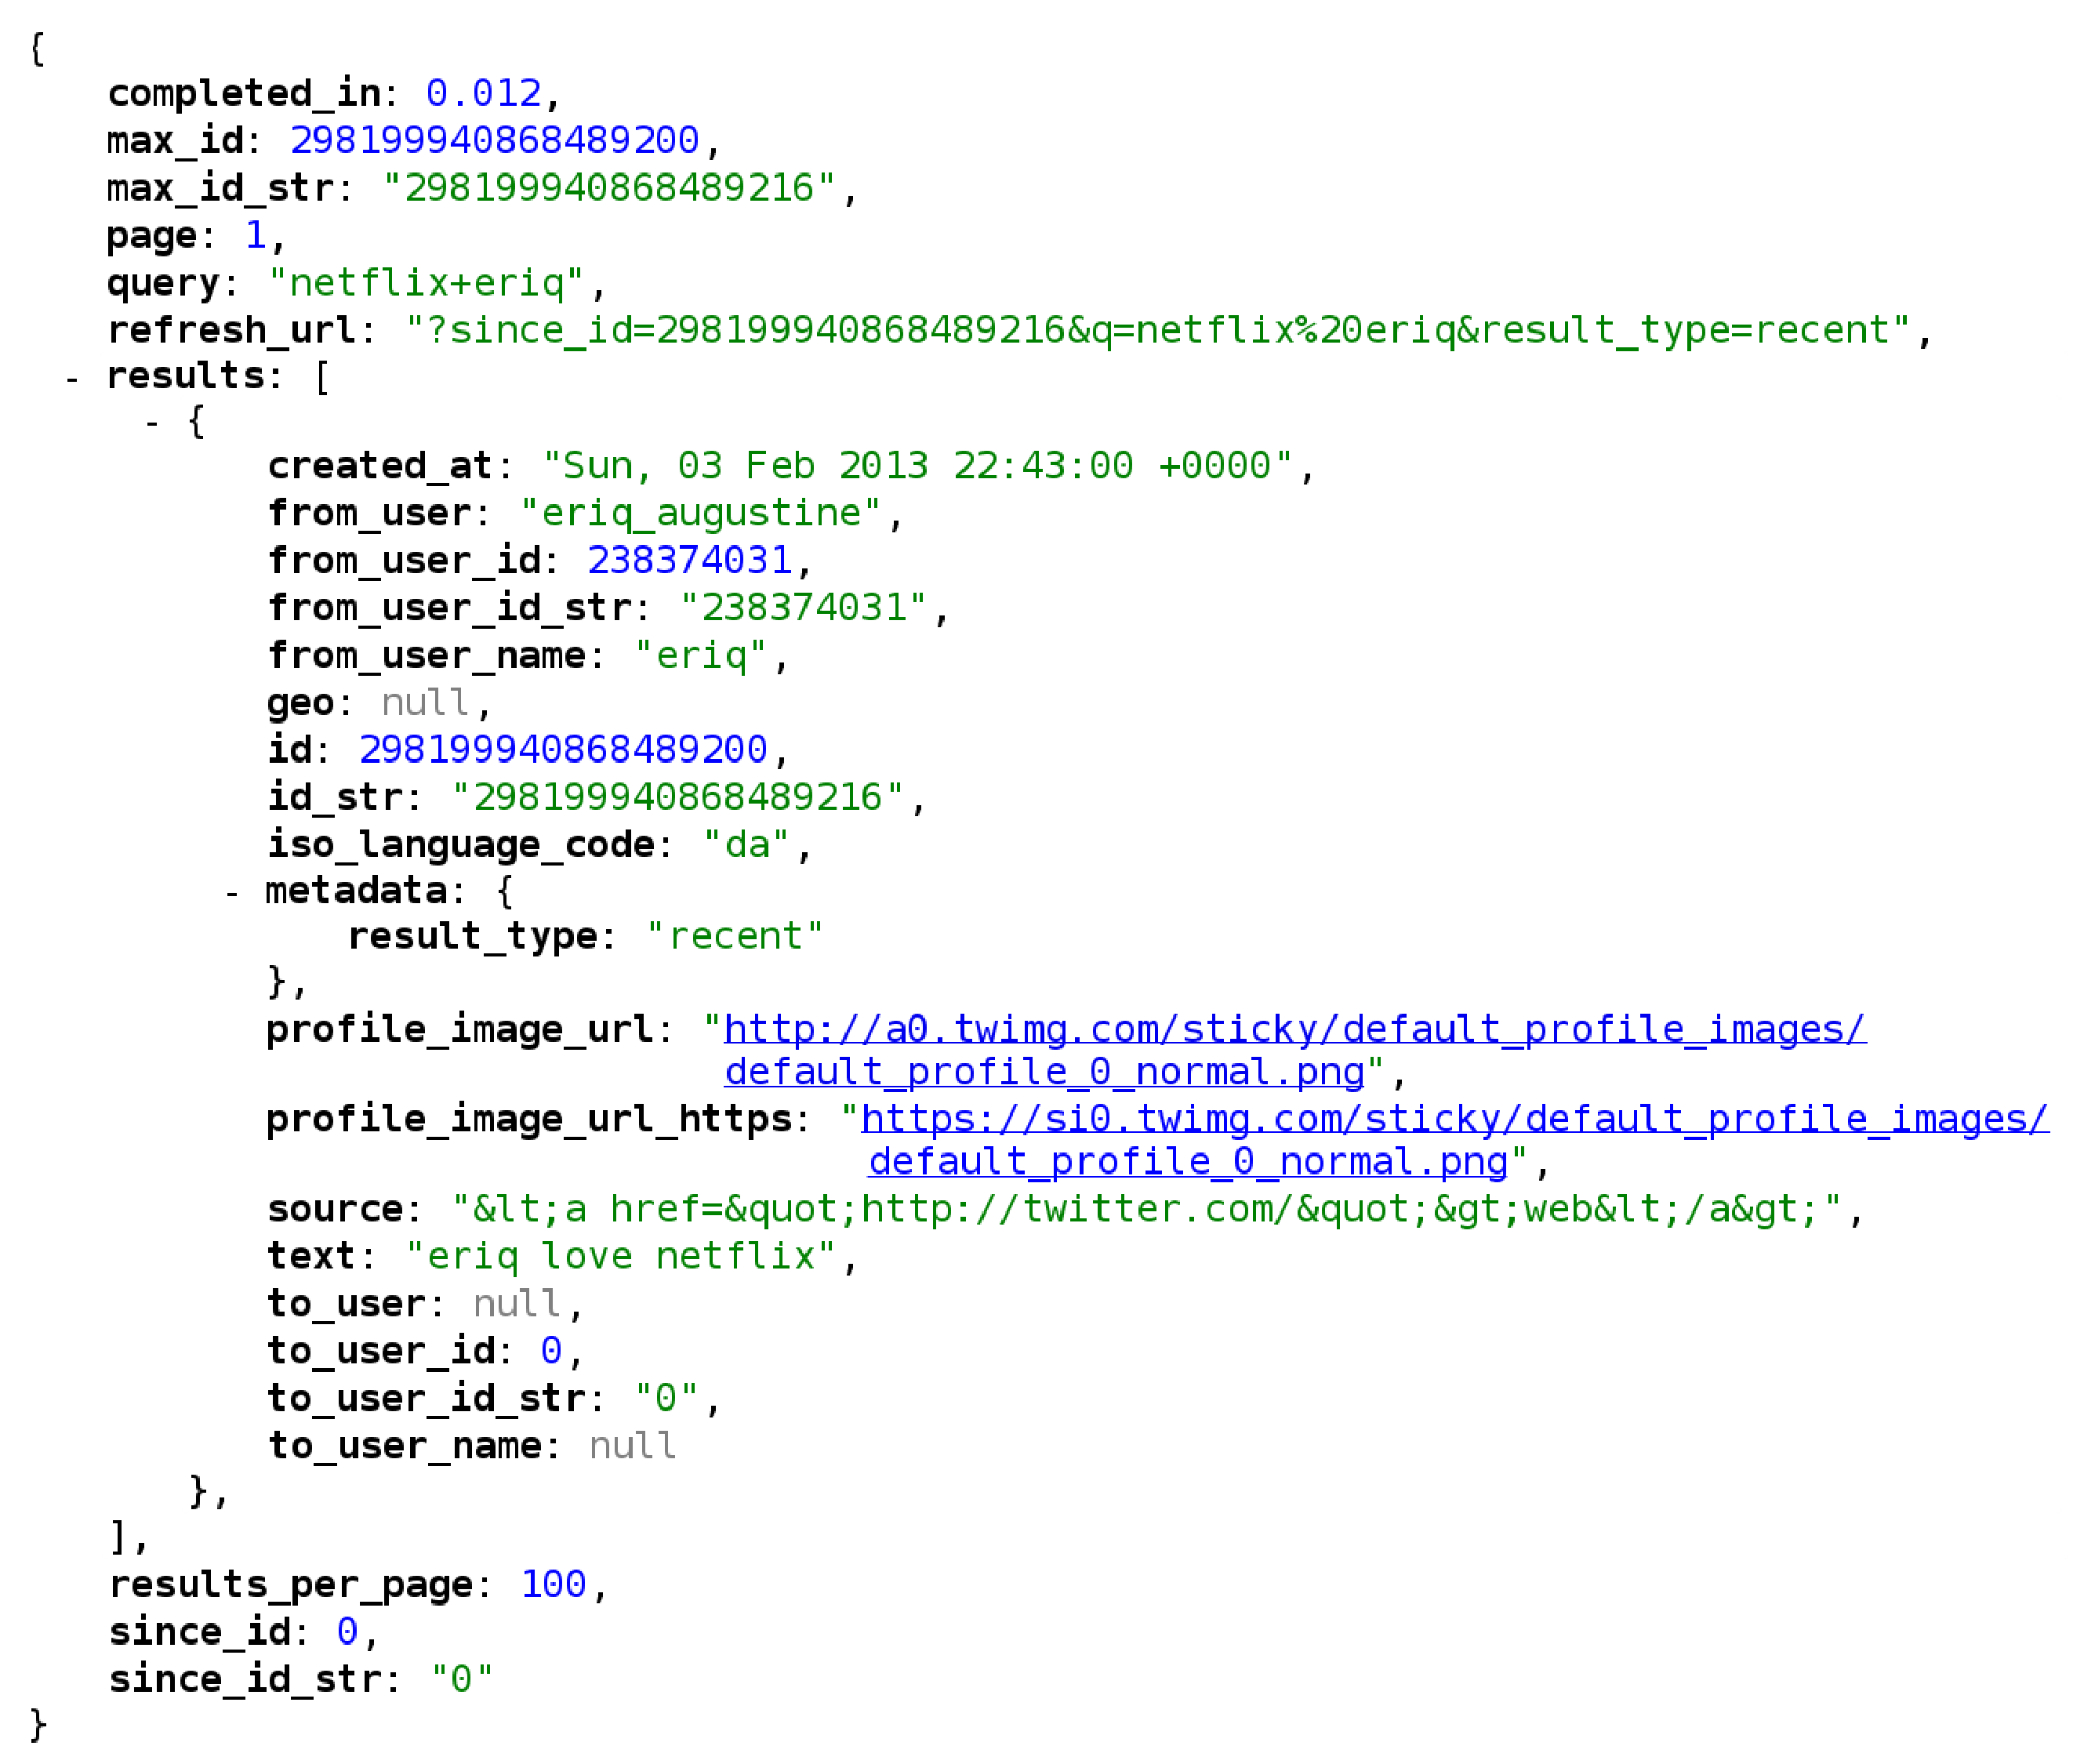
\includegraphics[width=150mm]{images/api_result.eps}
         \end{minipage}
      }
      \captionfonts
      \caption[Twitter Search API Result]{A JSON result from the Twitter Search API}
      \label{fig:apiRes}
   \end{center}
\end{figure}

Figure~\ref{fig:apiRes} shows the result from the query ``eriq netflix''. Notice that some fields,
like the \textsf{geo} field, can be null. Also note that the API incorrectly guessed the language of the tweet as Danish.

\part{SPOONS Architecture}
\label{arch}

\begin{figure}
   \begin{center}
      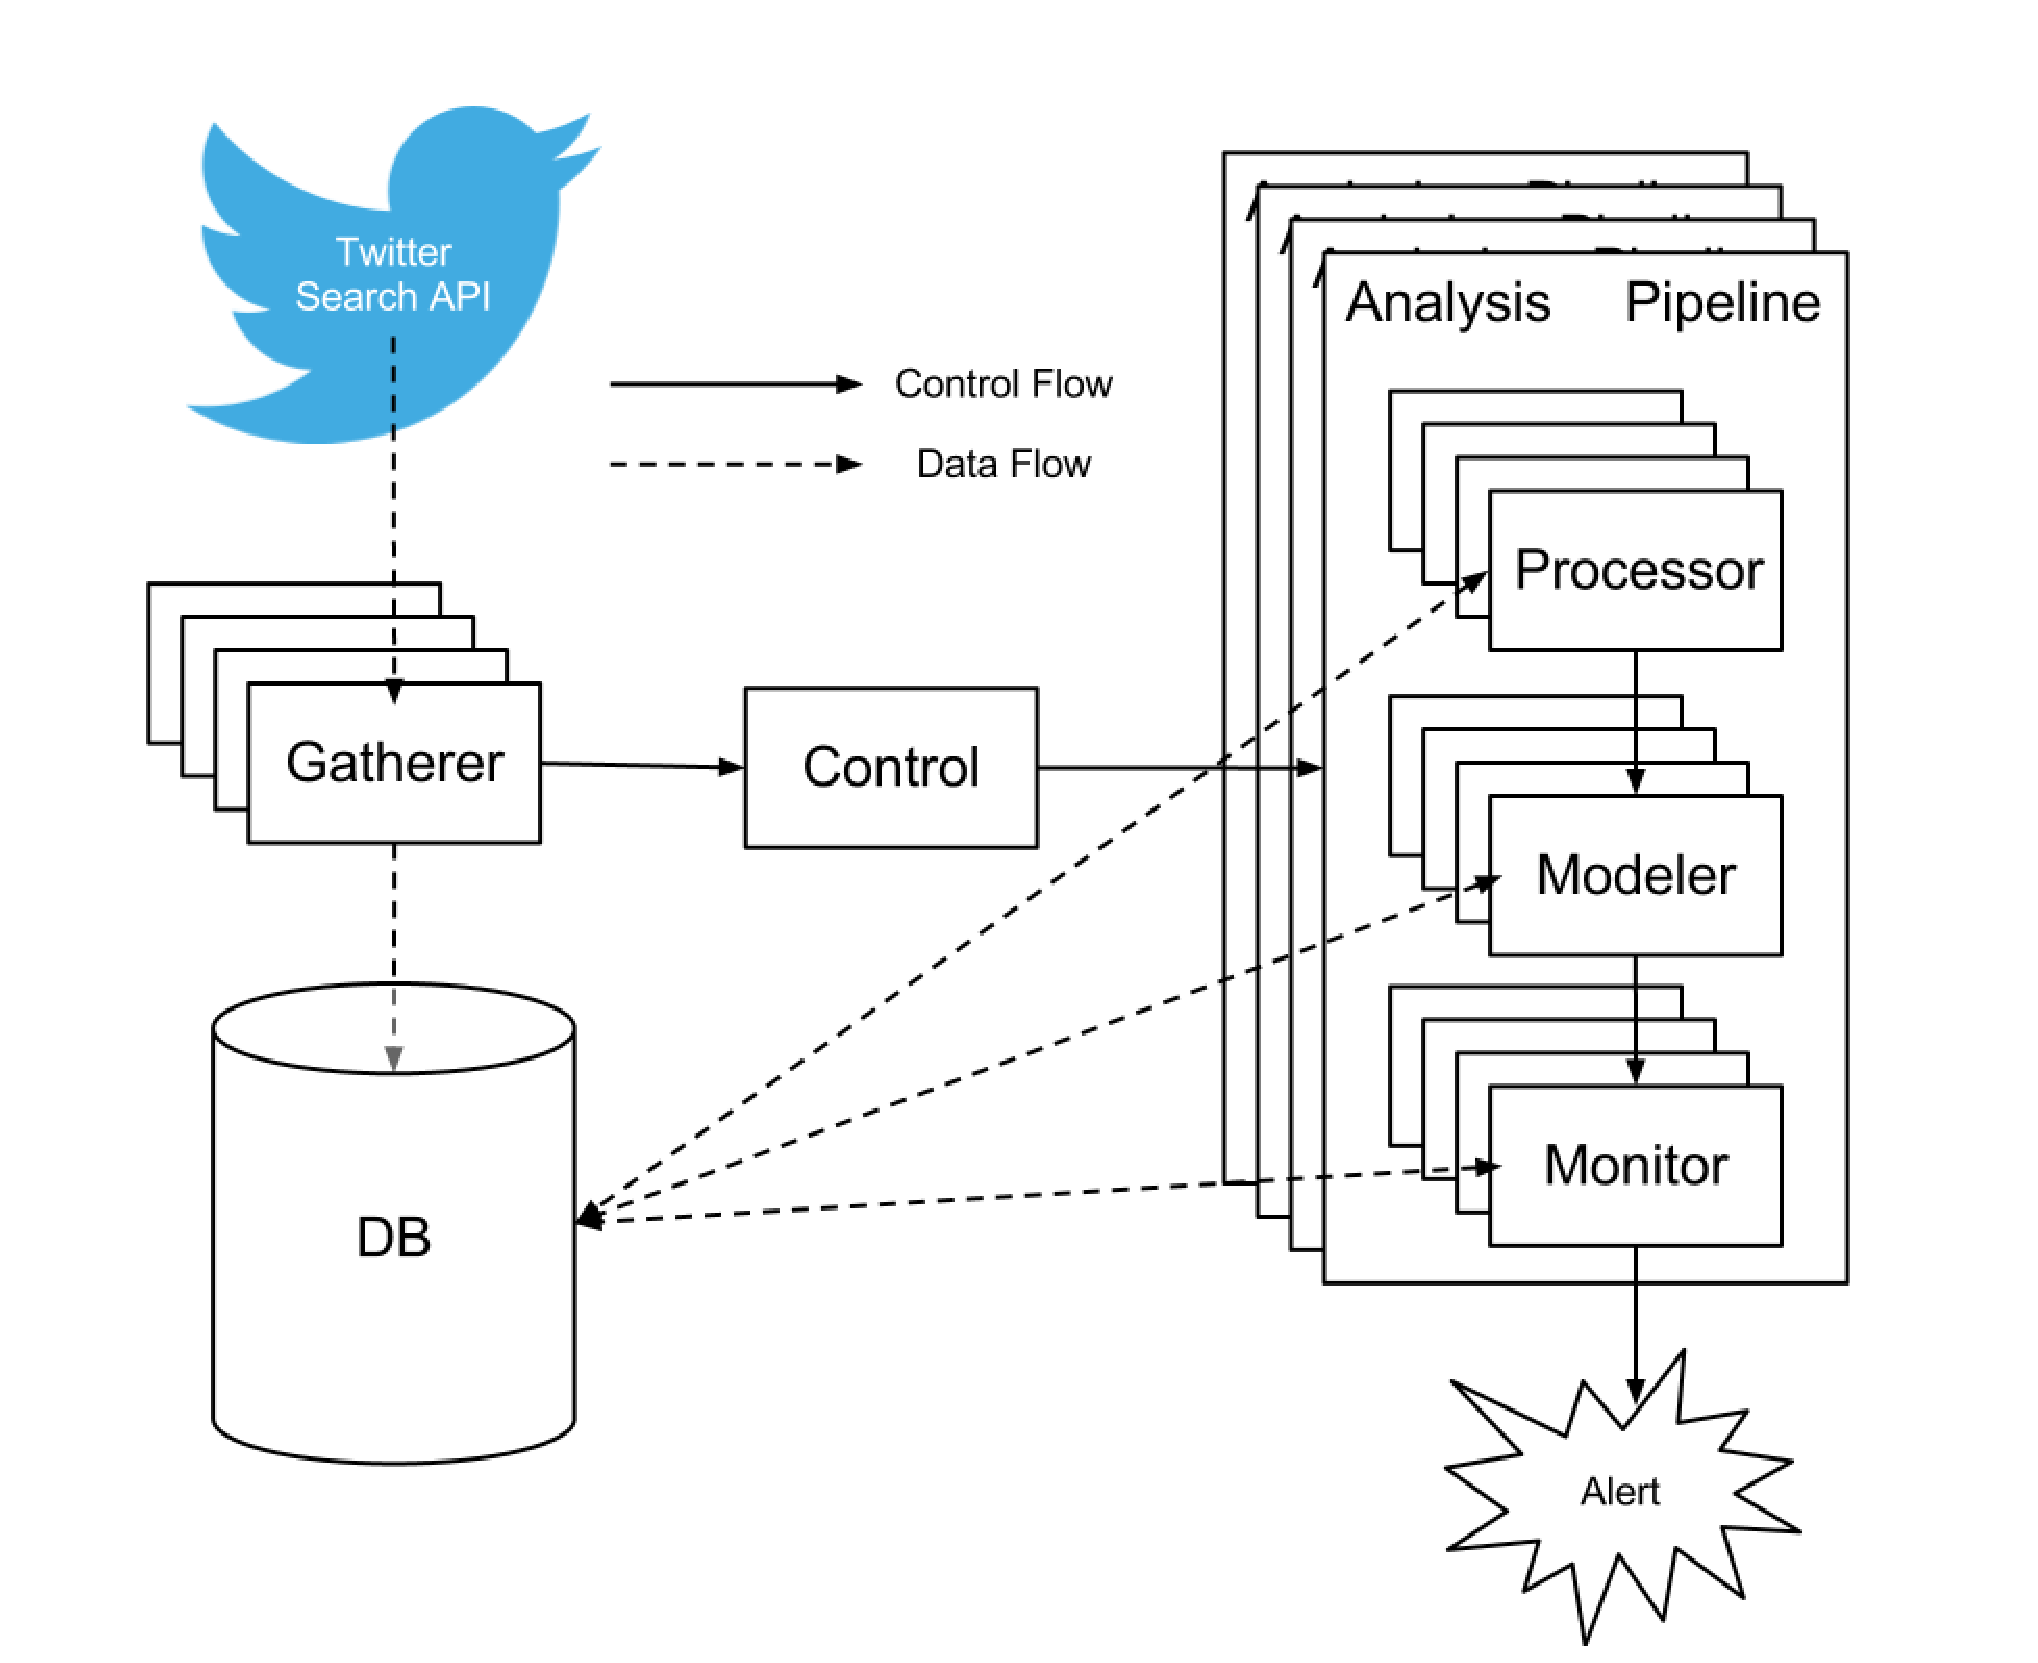
\includegraphics[width=0.8\textwidth]{images/SPOONS_Framework_Architecture.eps}
      \captionfonts
      \caption[SPOONS Framework Architecture]{The flow of control and data through the SPOONS framework system.}
      \label{fig:frameworkArch}
   \end{center}
\end{figure}

\begin{figure}
   \begin{center}
      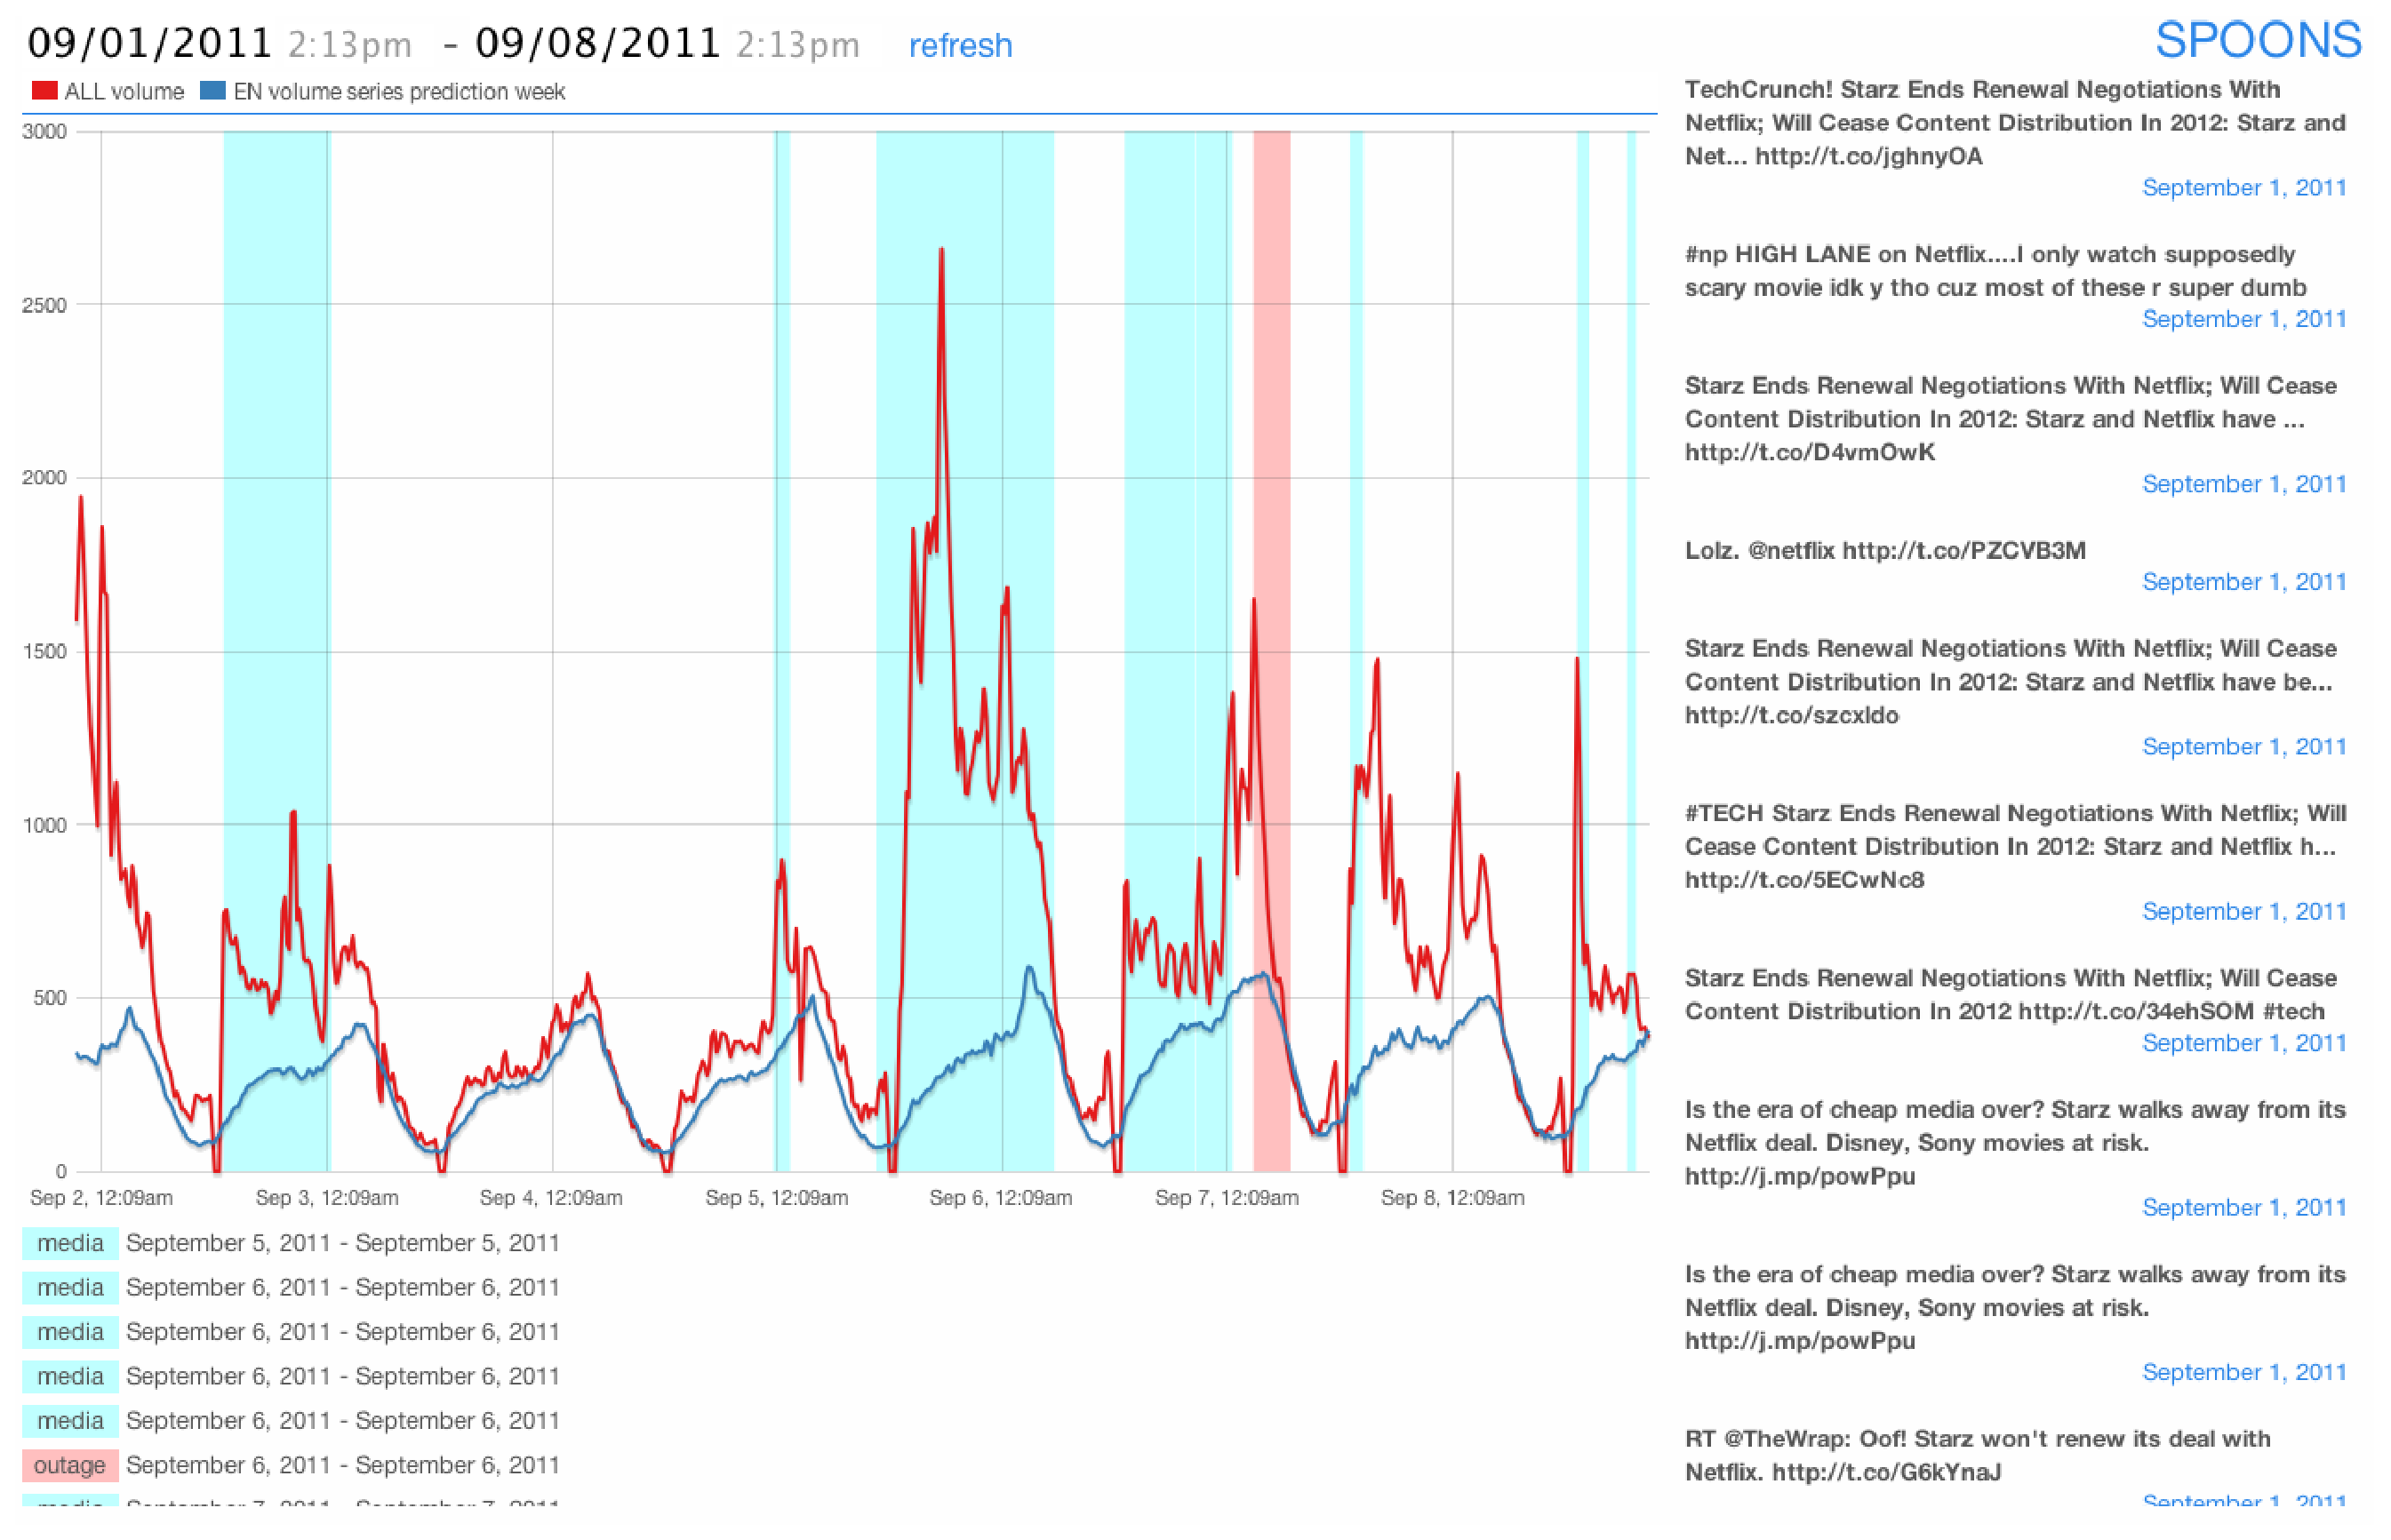
\includegraphics[width=0.8\textwidth]{images/ui.eps}
      \captionfonts
      \caption[SPOONS UI]{The web UI for SPOONS.}
      \label{fig:ui}
   \end{center}
\end{figure}

There are multiple levels of architecture within SPOONS that need to be discussed.
There is the Framework Architecture (Figure~\ref{fig:frameworkArch}) that describes the relations between the
different pieces of the framework; the Server Architecture (Figure~\ref{fig:serverArch}) that describes the layout of
the different servers involved in the SPOONS system; and the Distribution Model which describes how tasks are
distributed between the different servers.

\chapter{Framework Architecture}
\label{arch-framework}
This section describes the architecture of the SPOONS framework. The SPOONS framework includes all pieces of SPOONS
that take the data from gathering all the way through to final analysis.

\section{High Level Solution}
\label{arch-framework-highlevel}

The general solution taken by SPOONS consists of four main steps:

\begin{description}
   \item[Collect:]
      Tweets are collected from Twitter.
   \item[Process:]
      The tweets are converted from plain text to some form of information that can be analyzed.
   \item[Model:]
      Use the information generated from the previous step to build a mathematical model of the information.
      Use past information to predict what the current model of the data should look like.
   \item[Compare:]
      Compare the two models generated in the previous step. A significant divergence means that there is
      anomalous traffic.
\end{description}

\subsection{Framework Overview}
\label{arch-framework-highlevel-overview}

Figure~\ref{fig:frameworkArch} shows the flow of control and data through the SPOONS framework. Data comes into SPOONS
in the form of Tweets collected by the Gatherers, and leave SPOONS in the form of alerts generated by the Monitors.

\subsubsection{Gatherer}
Gatherers are responsible for collecting documents from a specified data source such as the Twitter Search API.

\subsubsection{Database}
After the tweets are gathered, they are placed in the database. In addition to storing just tweets, the database also stores
configuration data, intermediary calculations, and the results of the Analysis Pipelines.

\subsubsection{Control}
The Control is responsible for controlling the SPOONS server. It maintains data structures with all of the Gatherers and
Analysis Pipelines. It is also responsible for communication with other servers in the SPOONS cluster.

\subsubsection{Processor}
Processors are data transformation utilities that takes raw data and puts it in a form that other components can use.

\subsubsection{Modeler}
Modelers are responsible for building a mathematical model of the data and can be split into two groups: \textbf{Predictors} and \textbf{Counters}.
Predictors build a predictive model of the data. Counters to build a model of the data that was actually gathered by the system.

\subsubsection{Monitor}
Monitors take the models produced by the Predictors and Counters and compares them. The Monitors are responsible for
making the final decision on about a period of time being anomalous.

\section{Gatherers}
\label{arch-gatherers}
The data enters SPOONS at the Gatherers. The Gatherers run periodically (for Twitter, every two minutes).
Gatherers are asynchronous and not dependent on any other part of the framework. There may be multiple different
Gatherers running on the same machine. Gatherers are abstracted to be able to gather data from any source.
Once the Gatherers get their data, they place the data in the database and notify the Control that there is new data
available to the system.

\subsection{Twitter Holes}
\label{arch-twitter-holes}
It is worth noting that sometimes the Twitter Search API fails to return any data. We have not discovered the cause
of this, but Twitter does not report any errors. For unspecified amounts of time the Twitter API will just report zero
new tweets. We call these dead zones ``holes''. We have found that a query from a different IP usually does not
experience the same hole. To counteract holes, we run Gatherers on multiple servers and resolve uniques upon insertion
into the database.

\begin{figure}
   \begin{center}
      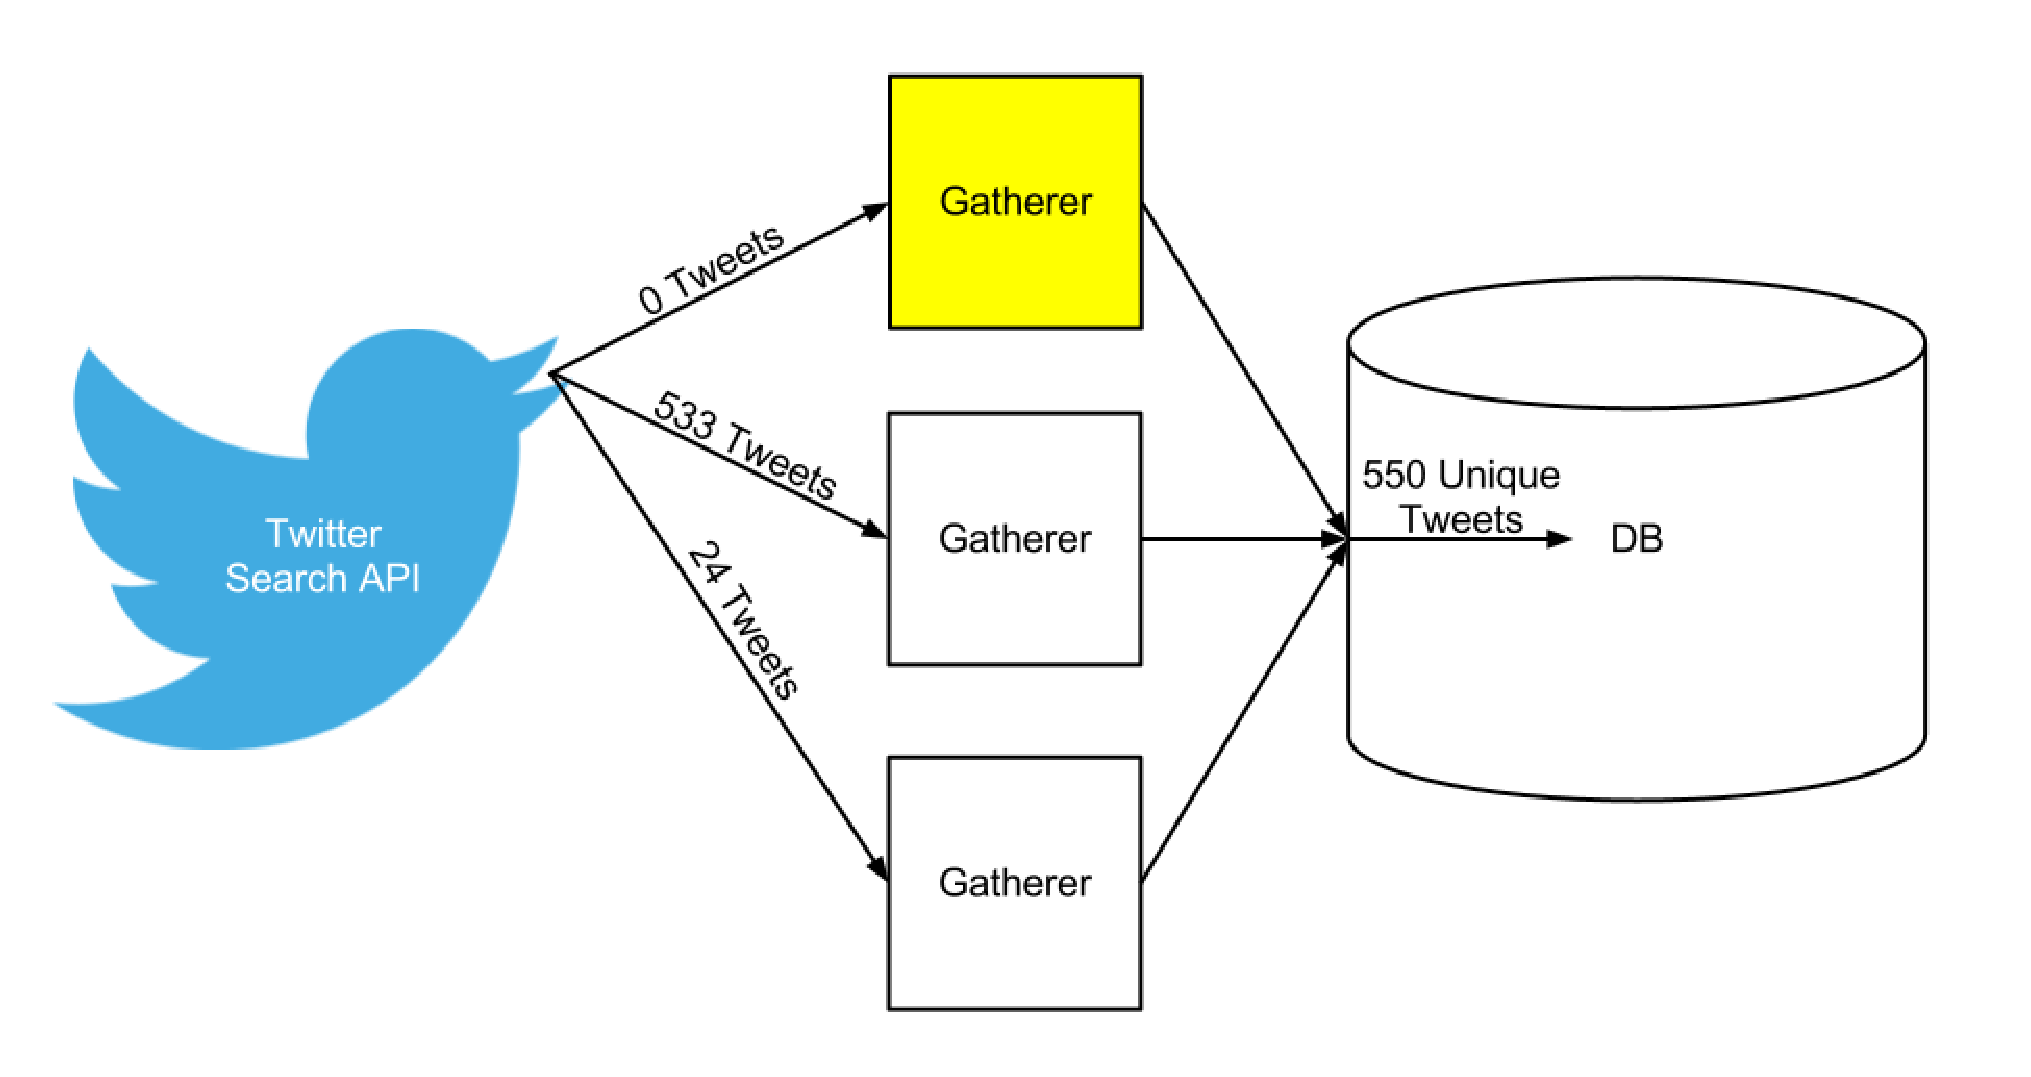
\includegraphics[width=0.9\textwidth]{images/Twitter_Holes.eps}
      \captionfonts
      \caption[Twitter Holes]{One server in a hole is covered by two other gathering servers.}
      \label{fig:ui}
   \end{center}
\end{figure}

\section{Processors}
\label{arch-processors}
Processors are responsible for processing or transforming data before it goes into the analysis pipelines.
\begin{itemize}
   % TODO(eriq): Check refs after chapter/sections are changed.
   \item{\underline{Classifier Processors}:} There exists a Processor for every tweet classifier used in SPOONS (see Chapter~\ref{classifiers}.
   Because of the high number of classifiers used, these constitute the majority of Processors and form the largest unit of work in SPOONS.
   These Processors classify every tweet into one of the nine tweet categories discussed in Section~\ref{class-tweet-classes}.

   \item{\underline{Author Processors}:} The Author Processors extract the author of tweets and try to establish which authors are credible. These Processors are
   outside the scope of this work and are discussed in other work\cite{cailinThesis}.

   \item{\underline{Valence Processors}:} The Valence Processors assign a numeric ``happiness'' score to every tweet. How that score is produced is outside the
   scope of this work (see Section~\ref{future-work-kim}).

   \item{\underline{Document Frequency Processors}:} The Document Frequency Processors maintain term frequencies and inverse document frequencies for the collection
   of tweets in SPOONS.

\end{itemize}

Unlike most parts of the analysis pipeline, Processors are a shared resource. That is, multiple analysis pipelines
invoke the same Processors. However, it does not make sense to restart the processing once it is started, or to
start another instance of the same Processor for the same data. Processors have a finite amount of data to process and may be cumulative.
To make sure that no redundant work is done, Processors are singleton. When multiple threads call into a Processor to do work, the Processor will block
all incoming threads until the work is complete. Then, the Processor will release all of the threads that requested the work.
This model allows all the analysis pipelines to share the same Processor without any redundancies.

\section{Analysis Pipelines}
\label{arch-pipelines}
An Analysis Pipeline (also called Analysis Method) is the analytical center of the SPOONS framework.
Pipelies are split into Tasks (see Section~\ref{arch-tasks}) which are chunked units of work.
The exact number and types of Tasks used are different for each pipeline.

An Analysis Pipeline typically starts with running any number of Processors on the data.
Then, the pipeline invokes modelers on the data from the Processors. These modelers typically build models for the
actual data coming into SPOONS as well as predictive models.
Finally, the pipeline invokes tasks that assess the models produced in the previous
step and decides whether or not there is an anomaly.

Every Analysis Pipeline gets its own thread, and there is no interdependence between the different pipelines.
Currently, SPOONS usually runs more than 20 Analysis Pipelines at a time.

\section{Tasks}
\label{arch-tasks}
Tasks are the core unit of computation in SPOONS. Almost everything that can be ``run'' is a child of the Task base
class. Every Task gets its own thread, and callers into the Task may request that the task block the calling thread
until the Task is complete.

Tasks are singleton with respects to the leaf child class. Therefore there are many tasks, but every task is
unique. We do this by enforcing that the class name is unique upon construction. The uniqueness of tasks is very
important to SPOONS distribution model that will be discussed in Section~\ref{arch-dist}.

\section{Modelers}
\label{arch-modelers}
Modelers are Tasks that are responsible for building a mathematical representation for the data.

\subsection{Predictors}
\label{arch-predictors}
Predictors build a predictive model of the data. For example, we have noticed that tweet volume tends to be
periodic day-to-day and week-to-week. Therefore, a Predictor may model that prediction by guessing that the volume
in the future will be the same as it was the previous week or day.

\subsection{Counters}
\label{arch-counters}
Counters attempt to build a model of data that was actually gathered by the system. Going with the previous example,
the Counter for modeling tweet volume would simply count the number of tweets gathered for a period.

\section{Monitors}
\label{arch-monitors}
Monitors take the models produced by the Predictors and Counters and compares them. The Monitors are responsible for
making the final decision about a period of time being anomalous.

\subsection{Auto-Tuning}
\label{arch-autotuning}
Monitors take anywhere from two to six tuning parameters. To find the best set of parameters, the Monitors can
automatically run themselves on a training set and search the space of all possible parameters. They then keep the
parameters that result in the best score.

\subsection{Resistance}
\label{arch-resistance}
A monitor's ``resistance'' is its tendency not to move into or out of an alert state.
The resistance is the number of normal or abnormal observations it needs to be
trigger a state change. Monitors are given resistance because otherwise outliers could cause
monitor to rapidly switch between alert and normal states.
There currently are three different methods of observing resistance.
The method of resistance as well as the resistance thresholds can also be auto-tuned.

\subsubsection{Fighting Resistance}
\begin{table}[H]
   \begin{center}
      \begin{tabular}{|c|p{9cm}|c|}
         \hline
            Parameter & Description & Restrictions \\
         \hline
            A & The number the counter must reach to enter an alert state. & $ A > 0 $ \\
         \hline
            R & The number the counter must reach to enter a normal state. & $ R > 0 $ \\
         \hline
      \end{tabular}
   \end{center}
\end{table}

Fighting resistance counts every time that there is a normal period as a +1, and every time there is
an anomalous period as a -1. If the counter reaches $-A$, then the monitor is put into an alert state.
If the counter reaches $R$, then the monitor is put into a normal state.

\subsubsection{Continuous Resistance}
\begin{table}[H]
   \begin{center}
      \begin{tabular}{|c|p{9cm}|c|}
         \hline
            Parameter & Description & Restrictions \\
         \hline
            A & The number the counter must reach to enter an alert state. & $ A > 0 $ \\
         \hline
            R & The number the counter must reach to enter a normal state. & $ R > 0 $ \\
         \hline
      \end{tabular}
   \end{center}
\end{table}

Continuous resistance must get $A$ continuous anomalous observations to enter an alert state, and $R$ continuous normal
observations to enter a normal state.

\subsubsection{Window Resistance}
\begin{table}[H]
   \begin{center}
      \begin{tabular}{|c|p{9cm}|c|}
         \hline
            Parameter & Description & Restrictions \\
         \hline
            W & The window size. & $ W > 0 $ \\
         \hline
            C & The number of anomalous observations necessary for an alert state. & $ 0 < C <= W $ \\
         \hline
      \end{tabular}
   \end{center}
\end{table}

Window resistance remembers $W$  previous observations as being normal or anomalous. If the number of anomalous
observations is or exceeds $C$, then an alert state is declared. Otherwise, the monitor stays in a normal state.

\subsection{Smoothers}
\label{arch-smoothers}
The monitors have a chance to smooth the data before it gets analyzed.
Smoothers take in a stream of data.
As with resistance methods, different smoothers and smoothing parameters can be auto-tuned.

\subsubsection{No Smoother}
Do not smooth. If this smoother is put into the parameter search space, then the effects of no smoothing can be seen.

\subsubsection{Moving Mean Smoother}
\begin{table}[H]
   \begin{center}
      \begin{tabular}{|c|c|c|}
         \hline
            Parameter & Description & Restrictions \\
         \hline
            W & The window size. & $ W > 0 $ \\
         \hline
      \end{tabular}
   \end{center}
\end{table}

The Moving Mean Smoother works by taking the mean in a sliding window of size $W$.
This Smoother tolerates a smaller window if there is not enough data available.
Therefore, this Smoother always outputs a number for every number in the input stream.

\section{Control}
\label{arch-control}
The Control is the center of a SPOONS instance. It handles the flow of all control and has the ability to start and
stop any task or pipeline on demand. It holds references to all the threads for the Gatherers and Analysis Pipelines.
The Control handles all the setup and tear down in the system.

There are different types of Controls that decide the behavior SPOONS on each respective server.
The Control is singleton with respects to the base class. Therefore, only one instance of any type of Control can be
active at any given time.

The Control is very careful to never allow anyone to own a reference to the currently running Control.
All requests to the Control are made statically to the ``Control'' base class. The base class then forwards the
request onto the specific instance of Control. We do this so that the rest of the SPOONS system never knows
what kind of Control is currently active. So we can switch a server between different roles without restarting the
system or notifying any other components of the SPOONS system.

All Controls always run the entire slate of Gatherers.

\subsection{Master Control}
\label{arch-master-control}
The Master Control is the Control that is responsible for the controlling SPOONS when it is in distributed mode.
The Master Control maintains information on all the active worker servers. It sends the worker servers
messages to tell them what work to do.

The Master Control maintains ``shallow execution'' of every pipeline in the system.
This means that this control runs each pipeline, but then distributes work for each pipeline as the work is generated.

\subsection{Worker Control}
\label{arch-worker-control}
Worker Controls do not take any initiative to run any tasks. Instead, they just wait for a Master Control to tell them what to do.

\subsection{Single Control}
\label{arch-single-control}
The Single Control is for a SPOONS instance that wants to run on a single server.

\section{Distributed Model}
\label{arch-dist}

\begin{figure}
   \begin{center}
      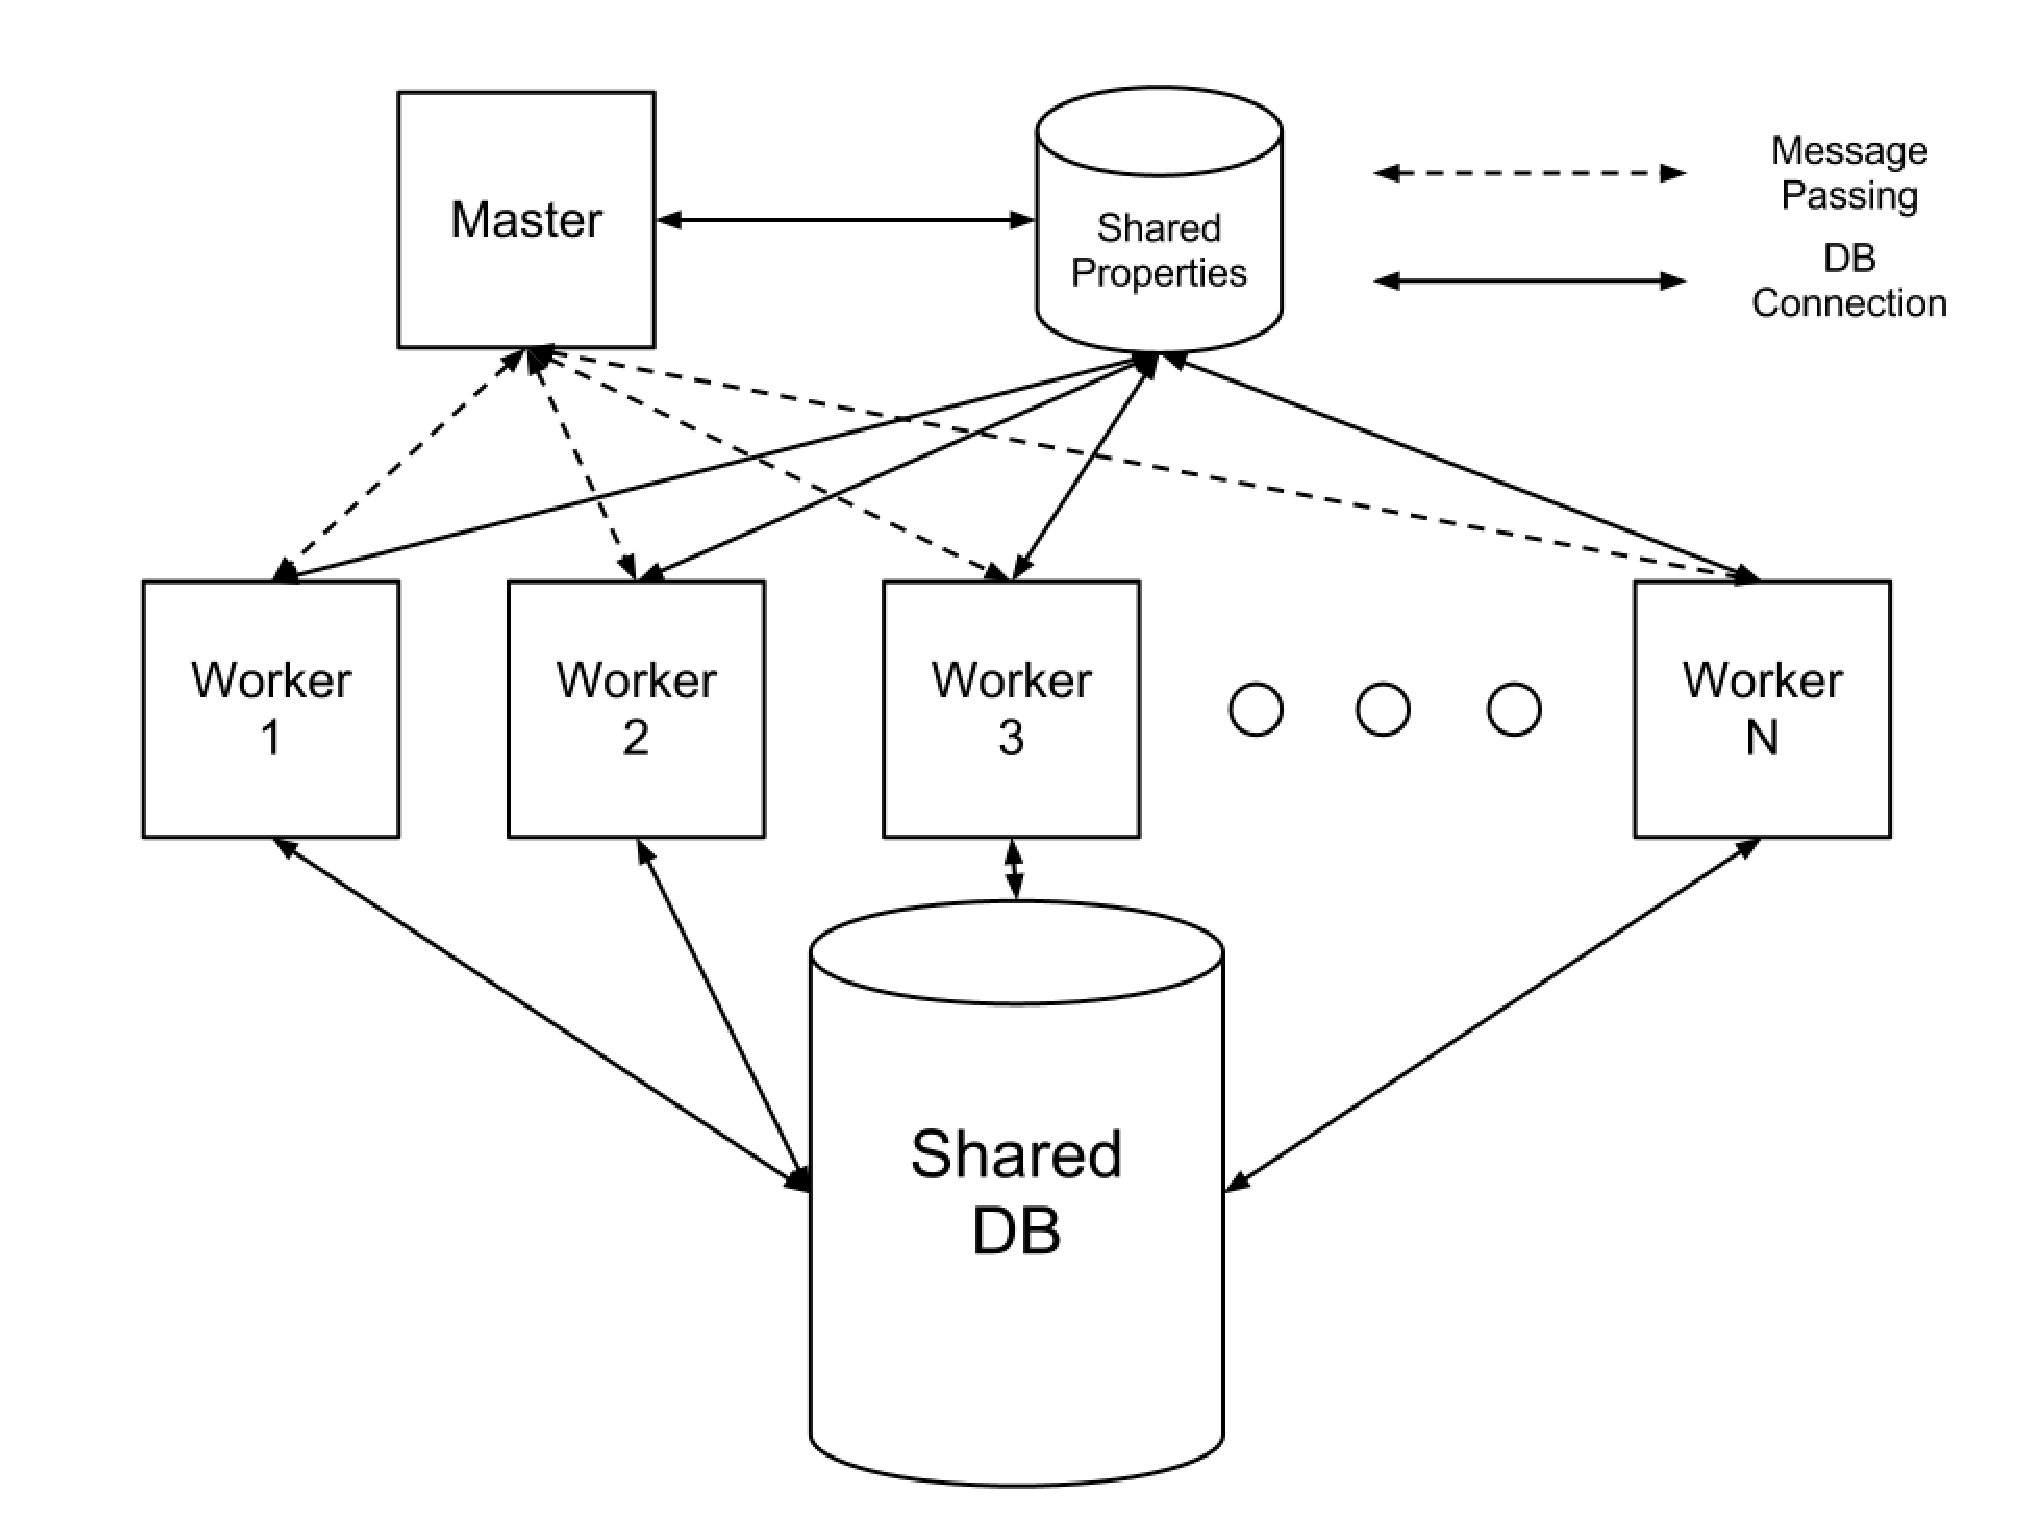
\includegraphics[width=0.8\textwidth]{images/SPOONS_Server_Architecture.eps}
      \captionfonts
      \caption[SPOONS Server Architecture]{The server architecture of the SPOONS system.}
      \label{fig:serverArch}
   \end{center}
\end{figure}

\begin{figure}
   \begin{center}
      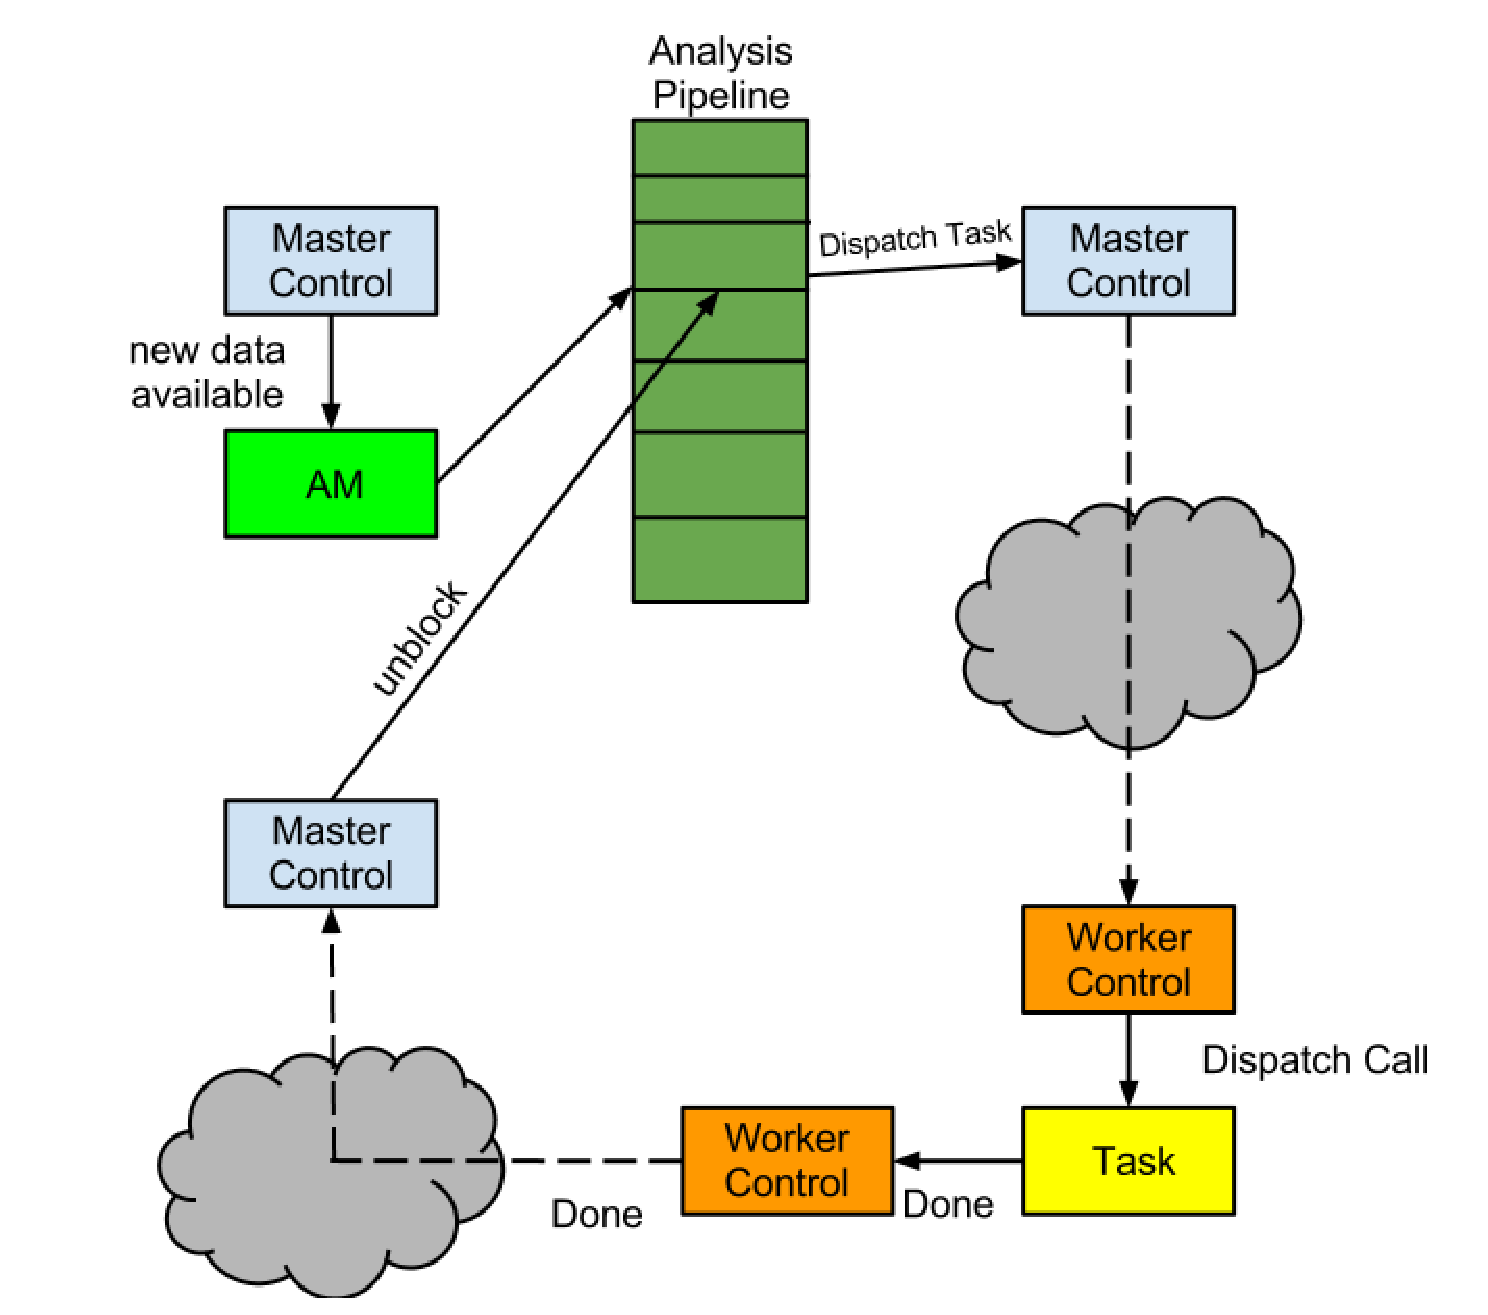
\includegraphics[width=0.8\textwidth]{images/SPOONS_Distributable_Task_Control_Flow.eps}
      \captionfonts
      \caption[SPOONS Distributable Task Flow]{The control flow for distributable tasks.}
      \label{fig:taskFlow}
   \end{center}
\end{figure}

As discussed before, SPOONS is a multi-server system (Fig~\ref{fig:serverArch}).
The SPOONS system uses the master/worker paradigm with a single master and N workers.

All of the servers share two primary resources: the primary database and a NoSQL property store.
When a master or worker comes online, it inserts an entry for itself into the shared property store.
If the new server is a worker, it alerts the current master about its existence, and visa-versa,
if the new server is a master. In addition, all workers are required to heartbeat to the master every
15 seconds and the master heartbeats to the workers every 15 seconds. Using this system, the master
always knowns about all of the workers and the worker always knows about the current master.
When a server misses three heartbeats, the server expecting that heartbeat assumes that the server has
gone down.

\subsection{Distribution Assumptions}
\label{arch-dist-assumptions}

The SPOONS distribution model relies on two assumptions about the system: every server contains
exactly the same data in memory and every Task can be uniquely referenced.

\subsubsection{Same Data}
SPOONS assumes that every server has the same data in memory on every server.
This means that not only does every server need to have the same data structures in memory,
but also that every server needs to have the same classes instantiated. The only exception to this
assumption is the Control. Depending on the role of the server, a different Control will be
instantiated. Because of this assumption, we do not have to worry about active replication
between servers or a worker being asked to do work that requires a class that is not instantiated.

\subsubsection{Uniquely Referenced Tasks}
As stated in Sec~\ref{arch-tasks}, Tasks are the basic unit of work inside SPOONS.
When a worker is told to execute some work, it is being asked to execute a specific task with specified
parameters. Therefore, Tasks need to be able to be referenced by a key that can be serialized and
sent over the wire from the master to the worker.

\subsection{Distributable Tasks}
\label{arch-dist-tasks}
Distributable Task is a subclass of Task that provides some of the distribution mechanism for Tasks.
When a task is to be distributed, the Distributable Task calls into the Control and requests that
the Control distributes it. The next step varies depending on the type of Control that is active:

\subsubsection{Master Control}
The task distributing control flow is described in Figure~\ref{fig:taskFlow}.
A Master Control blocks the calling thread and send a message to a selected worker\footnote{The
current scheduling algorithm chooses the worker that has the fewest tasks currently assigned to it.} telling to
run the task with given parameters. The message that goes to the worker just contains the task's unique identifier
and the parameters to the task's run. When the task is complete, the Worker Control sends the Task's return
status back to the Master Control. When the master receives a message from the worker that the requested task
has completed its run, it resumes the original calling thread and have it return with the return status given
by the worker.

\subsubsection{Worker Control}
Worker Controls do not distribute Tasks.
Because Tasks are atomic units of work, Tasks are not suppose to call other Tasks.
If Task A calls upon a Worker Control to distribute a Task B, then that means that Task A has violated
its own atomicity. This is considered a violation of the framework and will cause the Worker Control to throw an error.

\subsubsection{Single Control}
Instead of blocking the calling thread like in the Master Contol, a Single Control
will just use the calling thread to run the task. When the task is complete,
the Single Control will return control to the caller.

\subsection{Shared Properties}
\label{arch-props}
As previously stated, all servers must maintain a consistent in-memory view of the system.
This can be troublesome if a Task needs to maintain cumulative settings or member datum.
Not only will this data need to be consistent on all the servers, but it also needs to maintain this
data between starts and stop of the system. An Analysis Pipeline should be able to the stopped for an arbitrary amount
of time and then restarted without losing data or its place.

To enforce these restrictions, SPOONS uses a shared property store. The shared property store is a MongoDB server.
Whenever a Task needs to store member datum, it places the data in the shared store. Making the data available to any server in the cluser.
A Task can first be run to completion on Server A and then when new data is availble run on Server B.
Because the Task stores the necessary information in the shared property store,
Server B can have all the information gained from the run on Server A and not lose any positional information.

In addition to storing shared properties, the shared property store houses information on every active server.
When a server comes online, it queries the property store to find all the other active servers and inserts itself into
the store. If a server fails to heartbeat, then the rest of the cluster that is still active will remove the entry for that server from the property store.

\chapter{Database}
\label{arch-database}
SPOONS is backed by a MySQL database. SPOONS currently uses 225 tables and 35 stored procedures. The 225 tables are further divided into
six different categories that are used in different stages of the analysis pipeline. In addition to tweets being stored in the database
configuration data, intermediary calculations, analysis results, and final alerting decisions are stored in the database. Keeping all of this
data allows the users to look back at any point in time for reference or debugging. The majority of the stored procedures are a bridge between
the UI and database. The stored procedures provide a consistent interface for the UI without the need to underlying details.

The database uses naming and schema conventions to maintain organization on its tables. The naming and schema conventions allow different
components of the Analysis Pipeline to be interchanged without any need to change/reprocess the data. In addition the conventions allows the UI
to represent new tables without the need for specifying them.

\section{Tables and Schemas}
\label{arch-database-tables}
Each stage in an analysis pipeline generally stores some information in the database. Because each stage generally deals with similar
types of data, these tables are considered to be in the same group. We enforce group membership using hints in the table names. For example, the
table name ``\textcolor{red}{RESULT}\_\textcolor{orange}{EN}\_\textcolor{yellow}{class}\_\textcolor{green}{heuristic}\_\textcolor{blue}{bayes\_net}''
gives five hints as to the type of the table.

\begin{enumerate}
   \item \textcolor{red}{RESULT} - Marks this table as a result table. This means that it is guaranteed to be shown in the UI.
   \item \textcolor{orange}{EN} - The language of the tweets that were input into this method.
   \item \textcolor{yellow}{class} - Indicates that this these results are output from a tweet classifier.
   \item \textcolor{green}{heuristic} - States that the type of classifier used was a heuristic classifier.
   \item \textcolor{blue}{bayes\_net} - The name of the classifier used.
\end{enumerate}

Using all of these hints, the UI can then ask for data for specific types of tables (eg. all result tables that are for English tweets).

The six different top level categories that SPOONS recognizes are:

\begin{enumerate}
   \item CALC - These are intermediary tables in analysis pipelines. CALC tables are typically only used when large sets of past data are needed for cumulative models. They are never shown to the UI.
   \item CONFIG - Contains information that analysis methods used to configure themselves before runs. These tables have been mostly replaced with the shared property store (see Section \ref{arch-props}).
   \item DATA - Raw input data. These tables are generally the output from the Gatherers.
   \item META - Contains information that is not analyzed, but required by the system. For example, the different classes that the classifiers use along with descriptions of each class.
   \item RESULT - These tables are output from some analysis pipeline. They are guaranteed to be shown in the UI.
   \item TEST - These tables are used for debugging and development. They are never shown in a user-facing UI, however may be shown in development UIs.
\end{enumerate}

The full schema for select tables are described in Appendix~\ref{appendix-db-schema}.

\subsection{Data Flow}
\label{arch-database-data-flow}
The flow of data through the different types of tables is described in Figure~\ref{fig:db-data-flow}.
The data originates from the Gatherers and is moved into DATA tables. Information from
DATA, CONFIG, and META tables are analyzed and placed in either CALC, RESULT, or TEST tables.
At a later time the data from CALC tables is further analyzed and the results are placed in a RESULT table.

\begin{figure}
   \begin{center}
      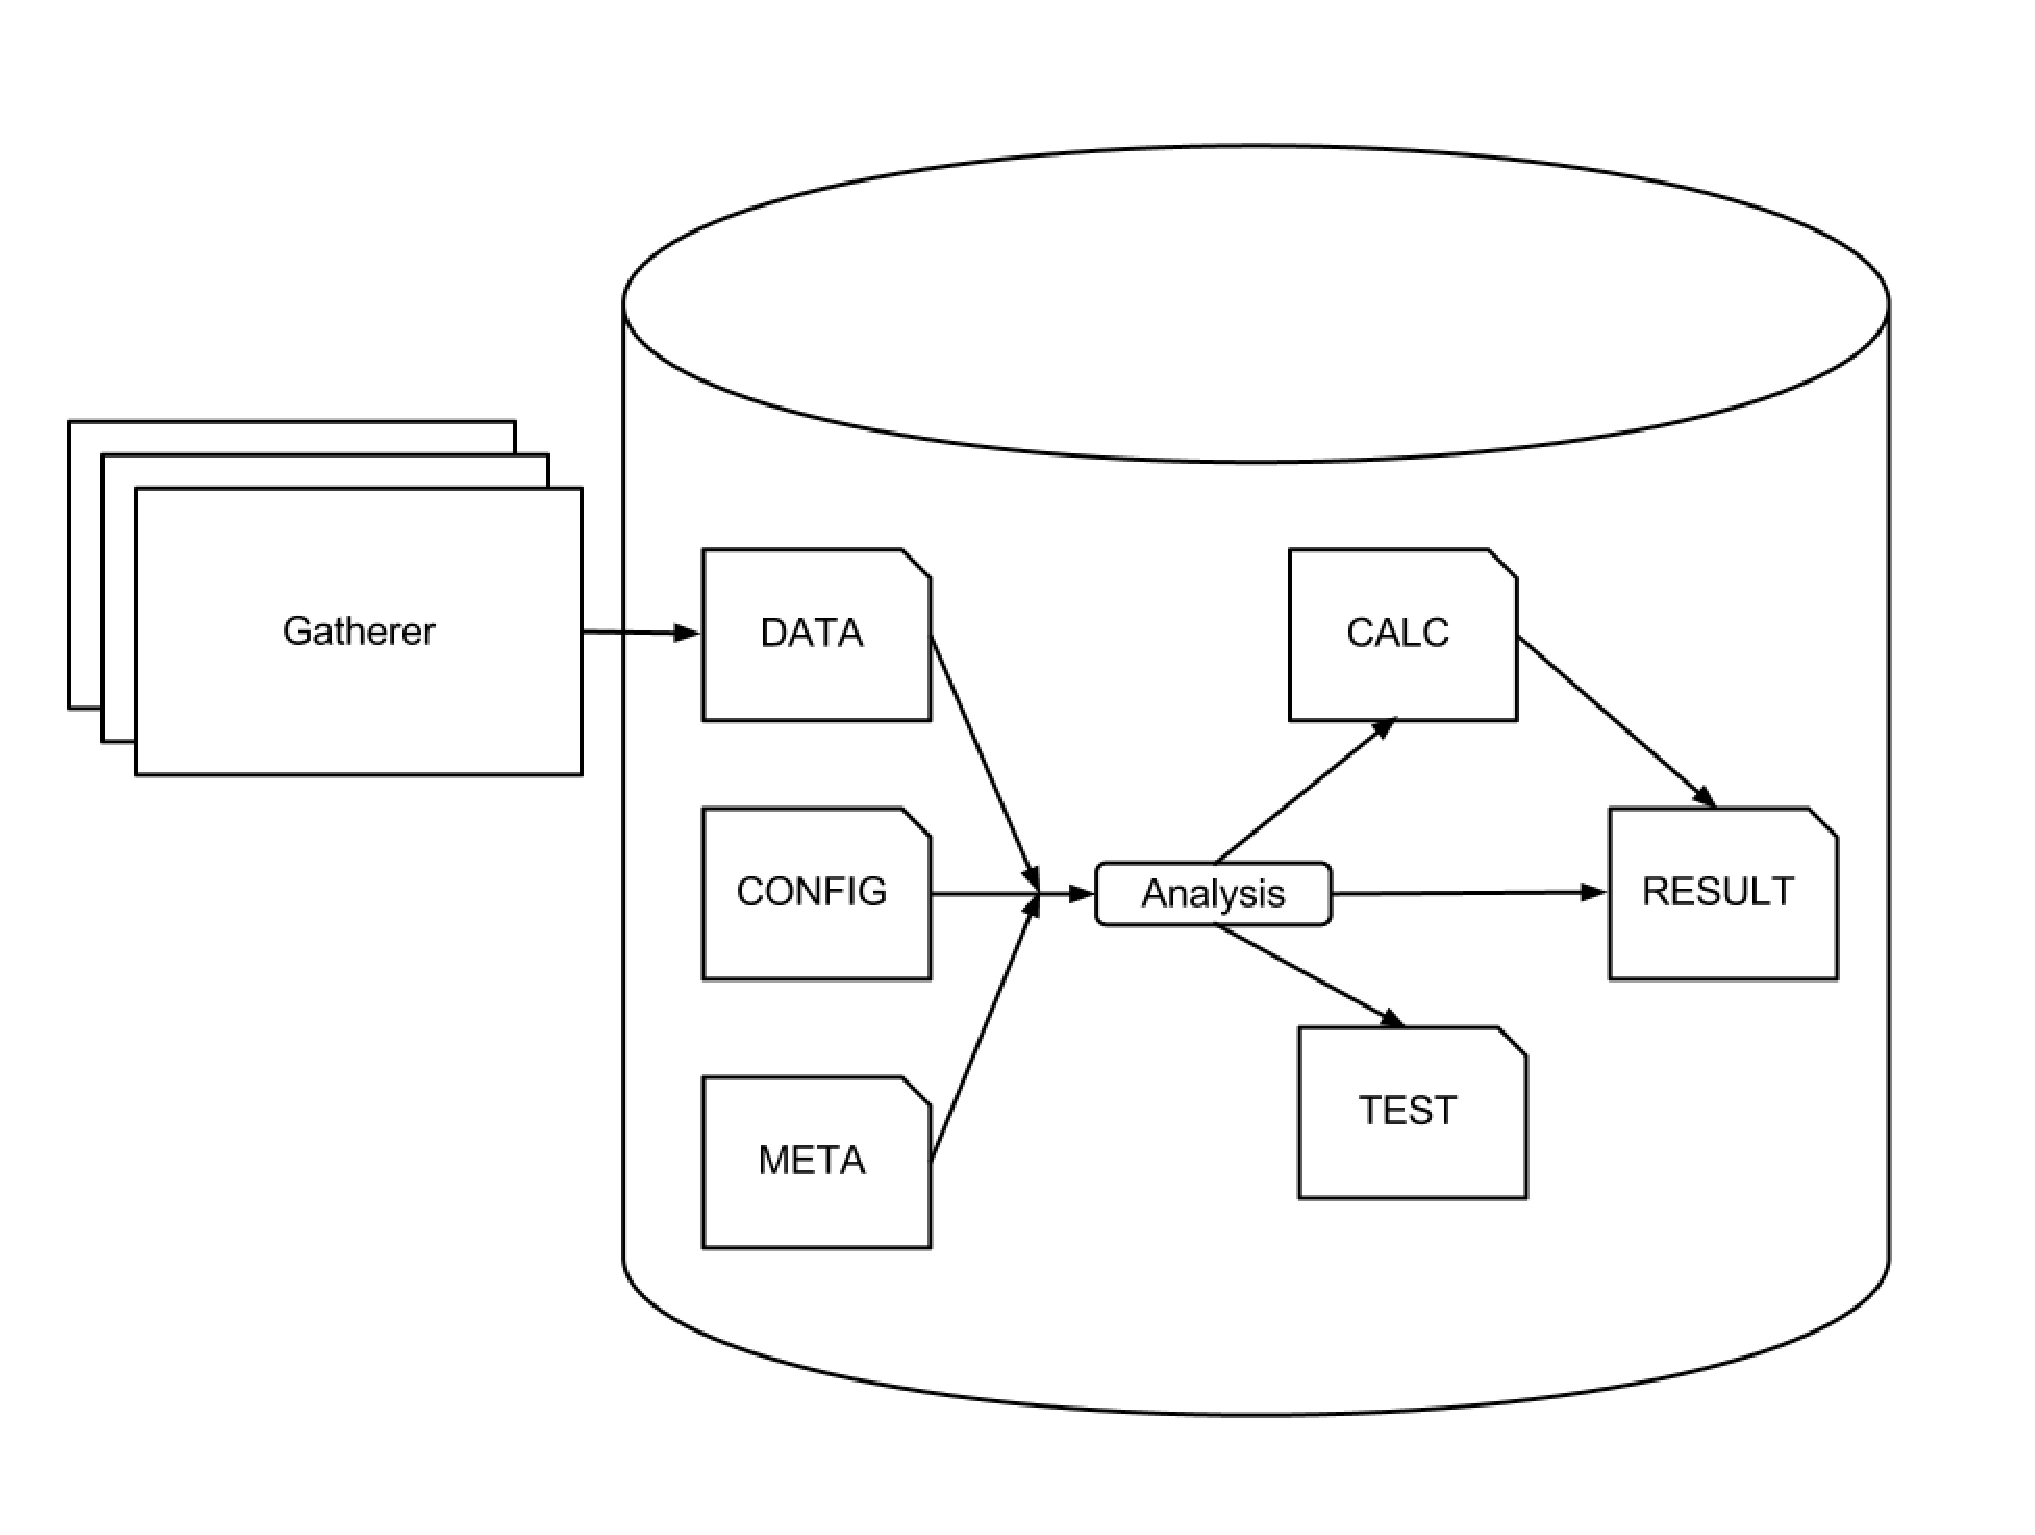
\includegraphics[width=0.8\textwidth]{images/DB_Data_Flow.eps}
      \captionfonts
      \caption[Database Data Flow]{The flow of data through the different types of tables in SPOONS.}
      \label{fig:db-data-flow}
   \end{center}
\end{figure}

\subsection{Tweets Table}
\label{arch-database-tables-tweets}
As the most used and important table in the database, the table that houses all of our tweets, ``DATA\_tweets'', gets special attention.

The tweets table contains ten attributes which are described in Table~\ref{table:tweet-attributes}.

\begin{table}
   \begin{center}
      \begin{tabular}{|l|p{12cm}|}
         \hline
            Name & Description
         \tabularnewline\hline
            \textsf{id} & An auto-incremented primary key.
         \tabularnewline\hline
            \textsf{twitter\_id} & The unique id Twitter gives a tweet.
         \tabularnewline\hline
            \textsf{published} & The epoch time that the tweet was posted according to Twitter.
         \tabularnewline\hline
            \textsf{content} & The raw content of the tweet.
         \tabularnewline\hline
            \textsf{source} & Information on where the tweet was posted from (eg. from a third party app).
         \tabularnewline\hline
            \textsf{lang} & The suggested language of the tweet.
         \tabularnewline\hline
            \textsf{author} & The author of the tweet.
         \tabularnewline\hline
            \textsf{frame\_id} & The frame that this tweet falls into, has an index on it.
         \tabularnewline\hline
            \textsf{place} & Information on where the tweet was posted from. This is a JSON structure and may contain fields such as ``city'' and ``state''.
         \tabularnewline\hline
            \textsf{geo} & Geographical coordinates of place.
         \tabularnewline\hline
      \end{tabular}
   \end{center}
   \caption[Database Tweet Attributes]{The database attributes used to describe tweets.}
   \label{tweet-attributes}
\end{table}

\subsubsection{Frames}
Inside SPOONS, we use a ``frame'' as the atomic unit of time. Currently, a frame corresponds to a minute. Bucketing the tweets into frames allows us to
gain a natural aggregation and smoothing. It also provides a natural index. Maintaining an index on \textit{frame\_id} allows quick retrieval of
time series data which is the primary task of SPOONS. Because insertions are generally chronological, insertions are also quick and do not require a
rebuild of the B-Tree index\cite{innodb}.

\section{UI Stored Procedures}
\label{arch-database-sp}
In addition to utility procedures, the database holds many stored procedures used by the UI.
This keeps the UI fairly stable in the face of database changes.

\subsection{Expected Schemas}
\label{arch-database-sp-schemas}
The UI Stored Procedures look for 6 distinct name/schema combinations all of which are required to be RESULT tables.
The different schema requirements are shown in Figure~\ref{fig:ui-expected-schema}, and described below:

\begin{table}
   \begin{center}
      \begin{tabular}{|l|p{12cm}|}
         \hline
            Schema Name & Required Columns
         \tabularnewline\hline
            Volume & \textsf{start\_frame}, \textsf{value}
         \tabularnewline\hline
            Volume Prediction & \textsf{start\_frame}, \textsf{prediction}
         \tabularnewline\hline
            Valence & \textsf{start\_frame}, \textsf{value}
         \tabularnewline\hline
            Valence & \textsf{start\_frame}, \textsf{prediction}
         \tabularnewline\hline
            Class & \textsf{start\_frame}, \textsf{undecided}, \textsf{media}, \textsf{neutral}, \textsf{snafu}, \textsf{watching}, \textsf{response}, \textsf{complaint}, \textsf{refuse\_to\_rate}, \textsf{happy}
         \tabularnewline\hline
            Group & \textsf{start\_frame}, \textsf{media}, \textsf{bad}, \textsf{other}
         \tabularnewline\hline
      \end{tabular}
   \end{center}
   \caption[Stored Procedure UI Expected Schema]{The different types of schemas that the UI looks for in RESULT tables.}
   \label{fig:ui-expected-schema}
\end{table}

%TODO(eriq): Not liking this V.
\begin{description}
   \item[Volume]
   This schema is for tables that contain time series information about tweet volumes.
   This includes tables that holds the time series for the total Netflix-related Twitter traffic.

   \item[Volume Prediction]
   These tables contain time series that are predictive models of Netflix-related Twitter traffic.

   \item[Valence]
   These tables contain time series for estimates of the current sentiment about Netflix.

   \item[Valence Prediction]
   These tables contain time series that are predictive models of the sentiment about Netflix.

   \item[Class]
   These tables contain time series for the volume of tweets that were classified into
   each of the nine categories described in Section~\ref{class-tweet-classes}.

   \item[Group]
   These tables contain time series for the volume of tweets that were classified into
   each of the thee different groupings described in Section~\ref{class-tweet-groups}.
\end{description}

The stored procedures will further divide the tables by language. The currently recognized languages are English,
Spanish, and Portuguese.

\part{Classifiers}
\label{classifiers}

\chapter{Why Classification?}
\label{class-why}
Classification helps discover Netflix service outages by differentiating between different types of Twitter traffic.

Figure~\ref{fig:normal-traffic} shows the normal pattern of Netflix-related Twitter traffic. The peaks appear at around 7pm
PST and the valleys are around 2am PST. This kind of pattern is very regular and repeats weekly during normal times. However
where there is some sort of event, the traffic develops spikes. Figure~\ref{fig:anomalous-traffic} shows a period with two
anomalous spikes. However, sampling tweets from the different spikes hints that the causes for the two different spikes
are very different. Figure~\ref{fig:linkless-traffic} shows tweets sampled from each spike. The left spike is composed mostly
of tweets indicating that Netflix is experiencing a service outage. The right spike however, is composed mainly of tweets linking to
a news article about Netflix. Therefore, we see that not only service outages generates spikes in Netflix-related Twitter traffic.

This is where classifiers become useful. If tweets can be placed into different classes according to the type of traffic that they
generate, then the different types of traffic can be differentiated. Figure~\ref{fig:classified-traffic} shows the result of classifying
the tweets and then building time series of the classes respective traffic. It becomes obvious that the spike on the left is caused by
outage related traffic and that the spike on the right is caused by media related traffic.

\begin{figure}
   \begin{center}
      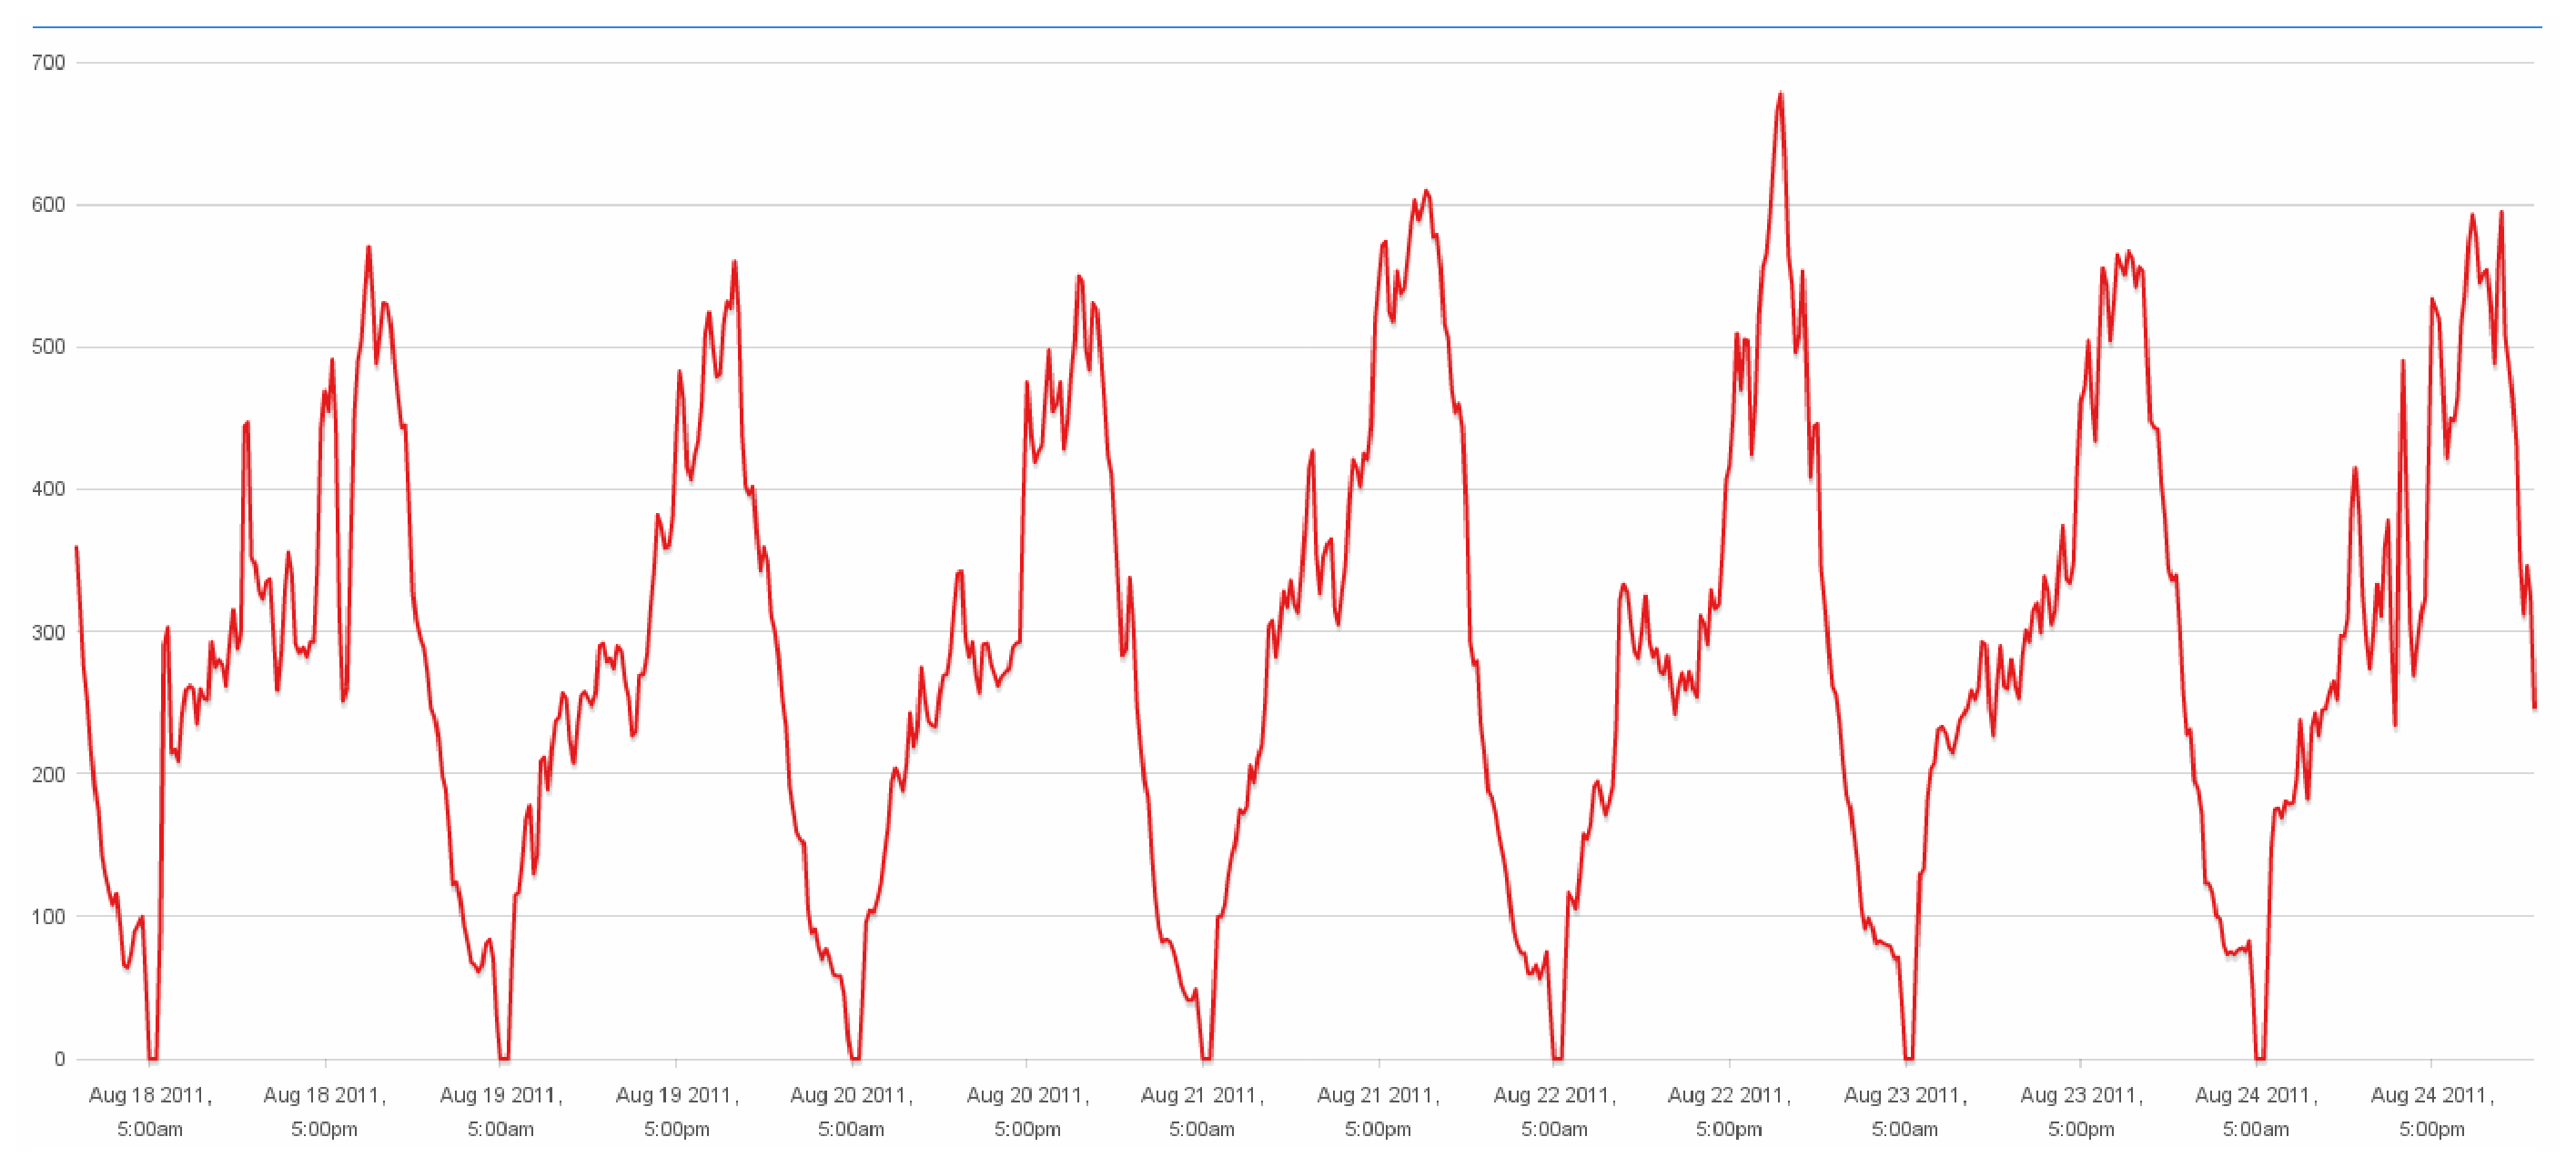
\includegraphics[width=0.8\textwidth]{images/Normal_Traffic.eps}
      \captionfonts
      \caption[Normal Traffic]{A weeks worth of Netflix-related Twitter traffic. Notice the daily periodicity.}
      \label{fig:normal-traffic}
   \end{center}
\end{figure}

\begin{figure}
   \begin{center}
      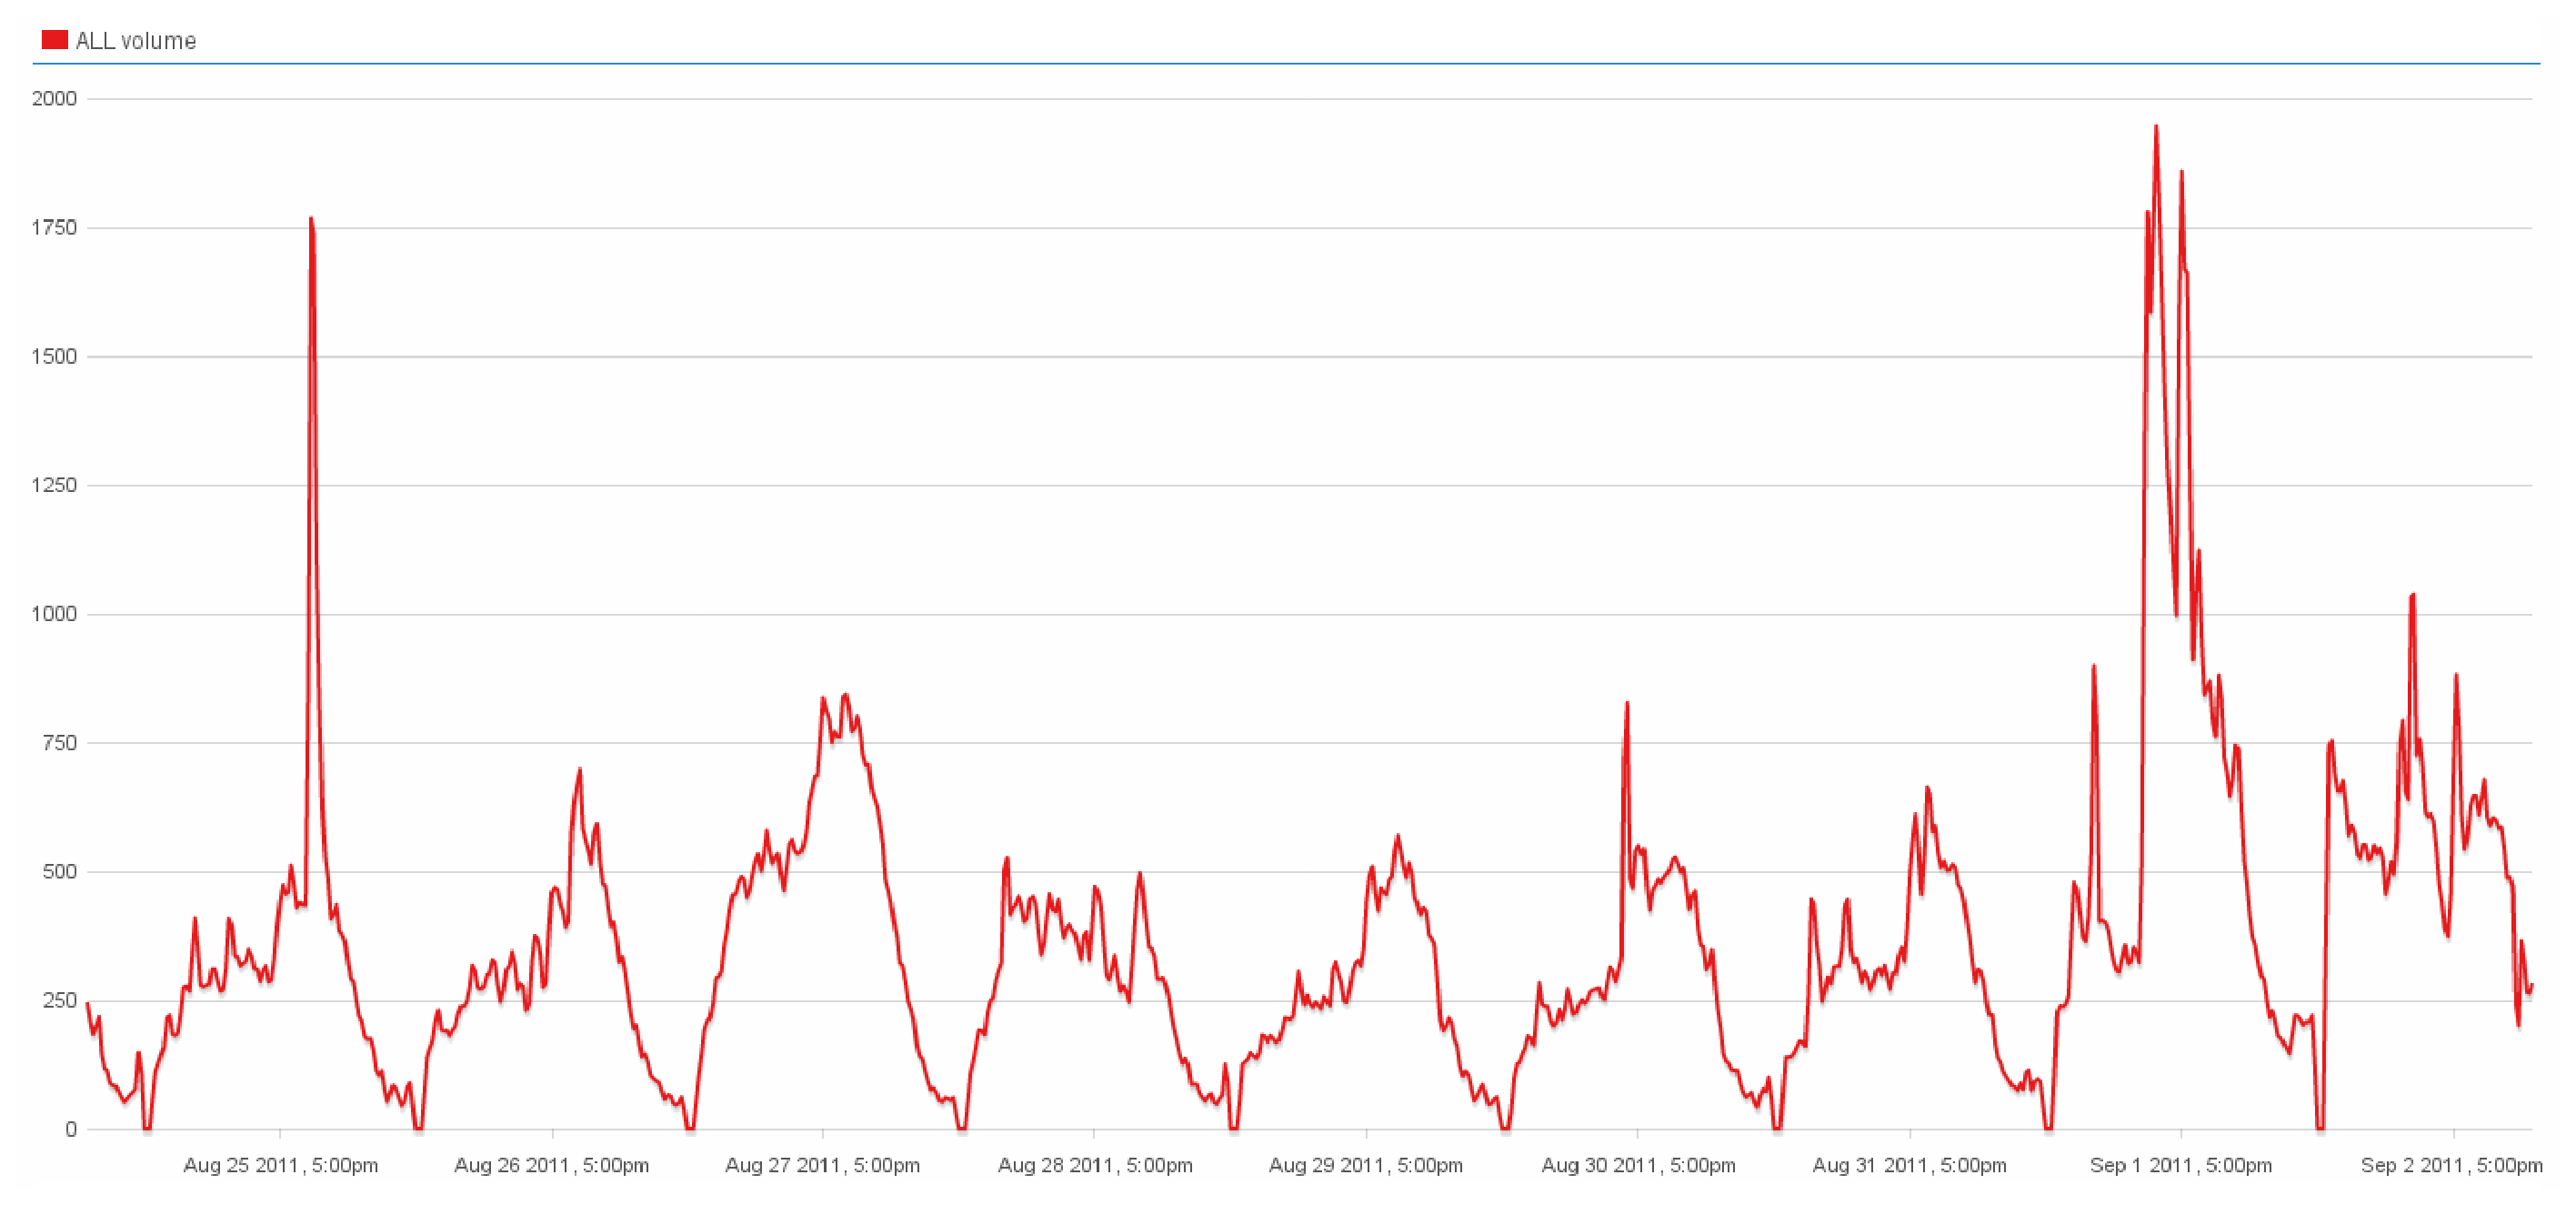
\includegraphics[width=0.8\textwidth]{images/Anomalous_Traffic.eps}
      \captionfonts
      \caption[Anomalous Traffic]{Netflix-related Twitter traffic with two different anomalies.}
      \label{fig:anomalous-traffic}
   \end{center}
\end{figure}

\begin{figure}
   \begin{center}
      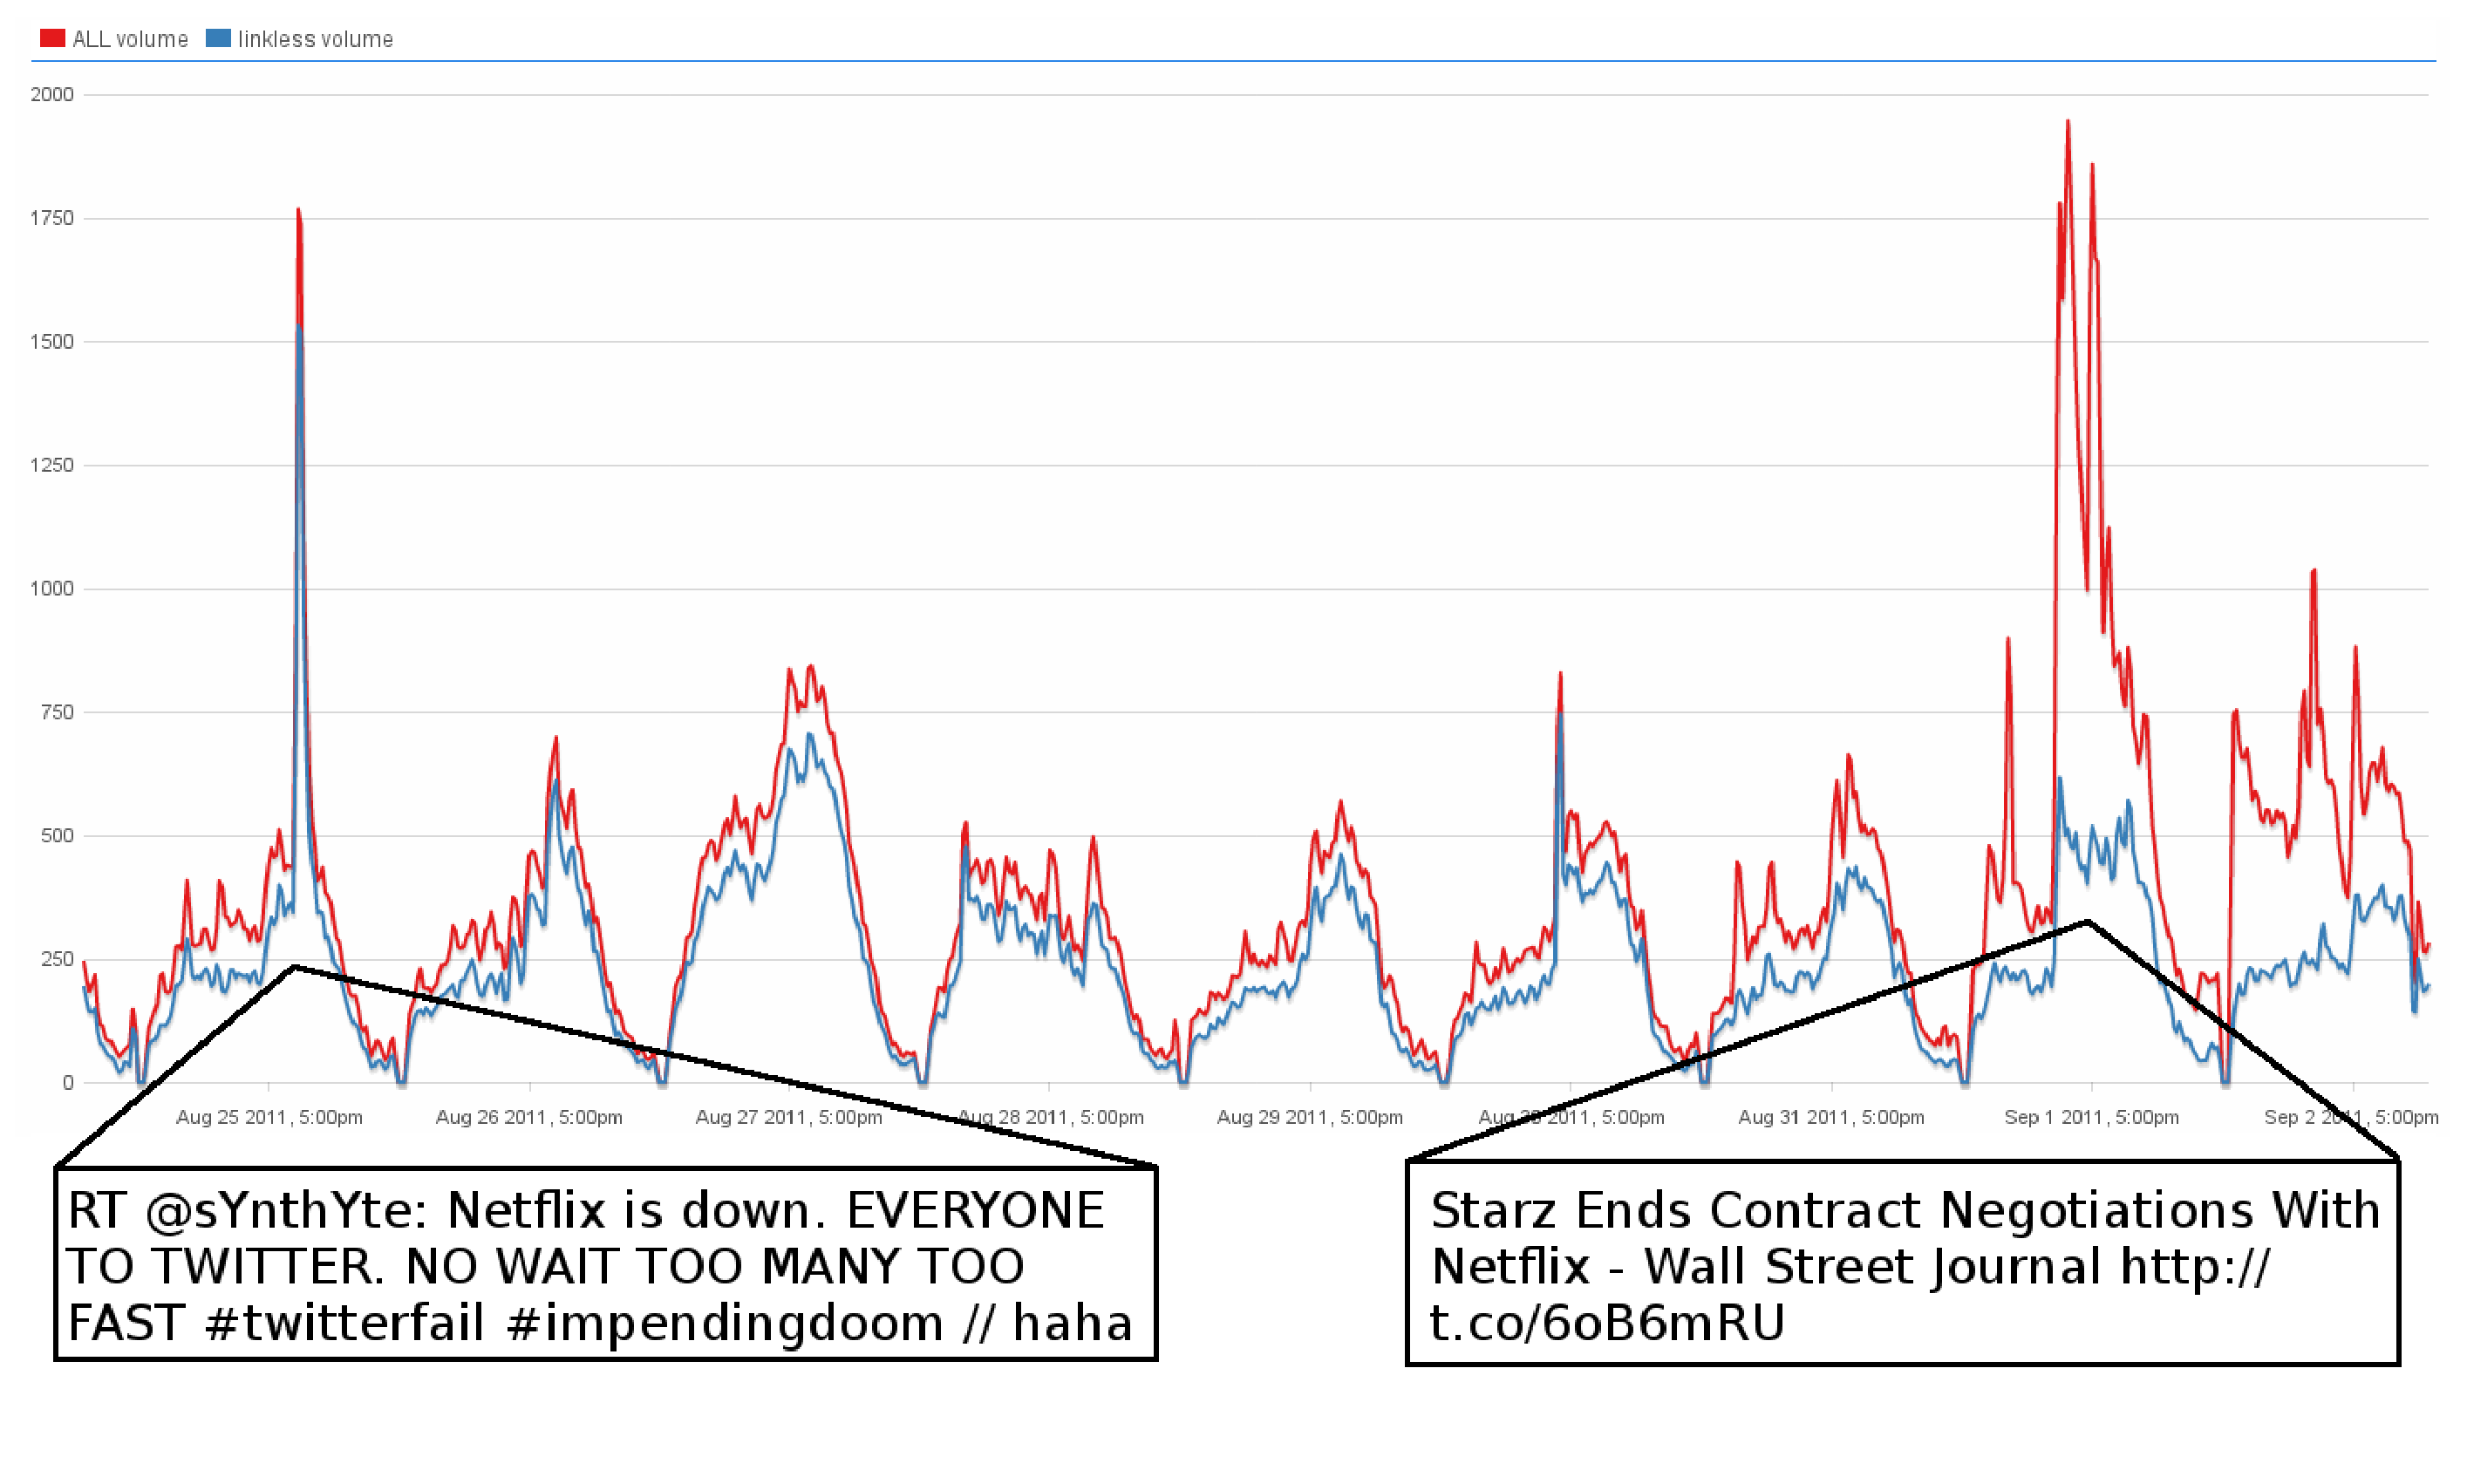
\includegraphics[width=0.8\textwidth]{images/Linkless_Differentiation.eps}
      \captionfonts
      \caption[Linkless Anomalous Traffic]{The same traffic shown in Figure~\ref{fig:anomalous-traffic}, with an additional line showing Netflix-related Twitter traffic that does not contain a URL.}
      \label{fig:linkless-traffic}
   \end{center}
\end{figure}

\begin{figure}
   \begin{center}
      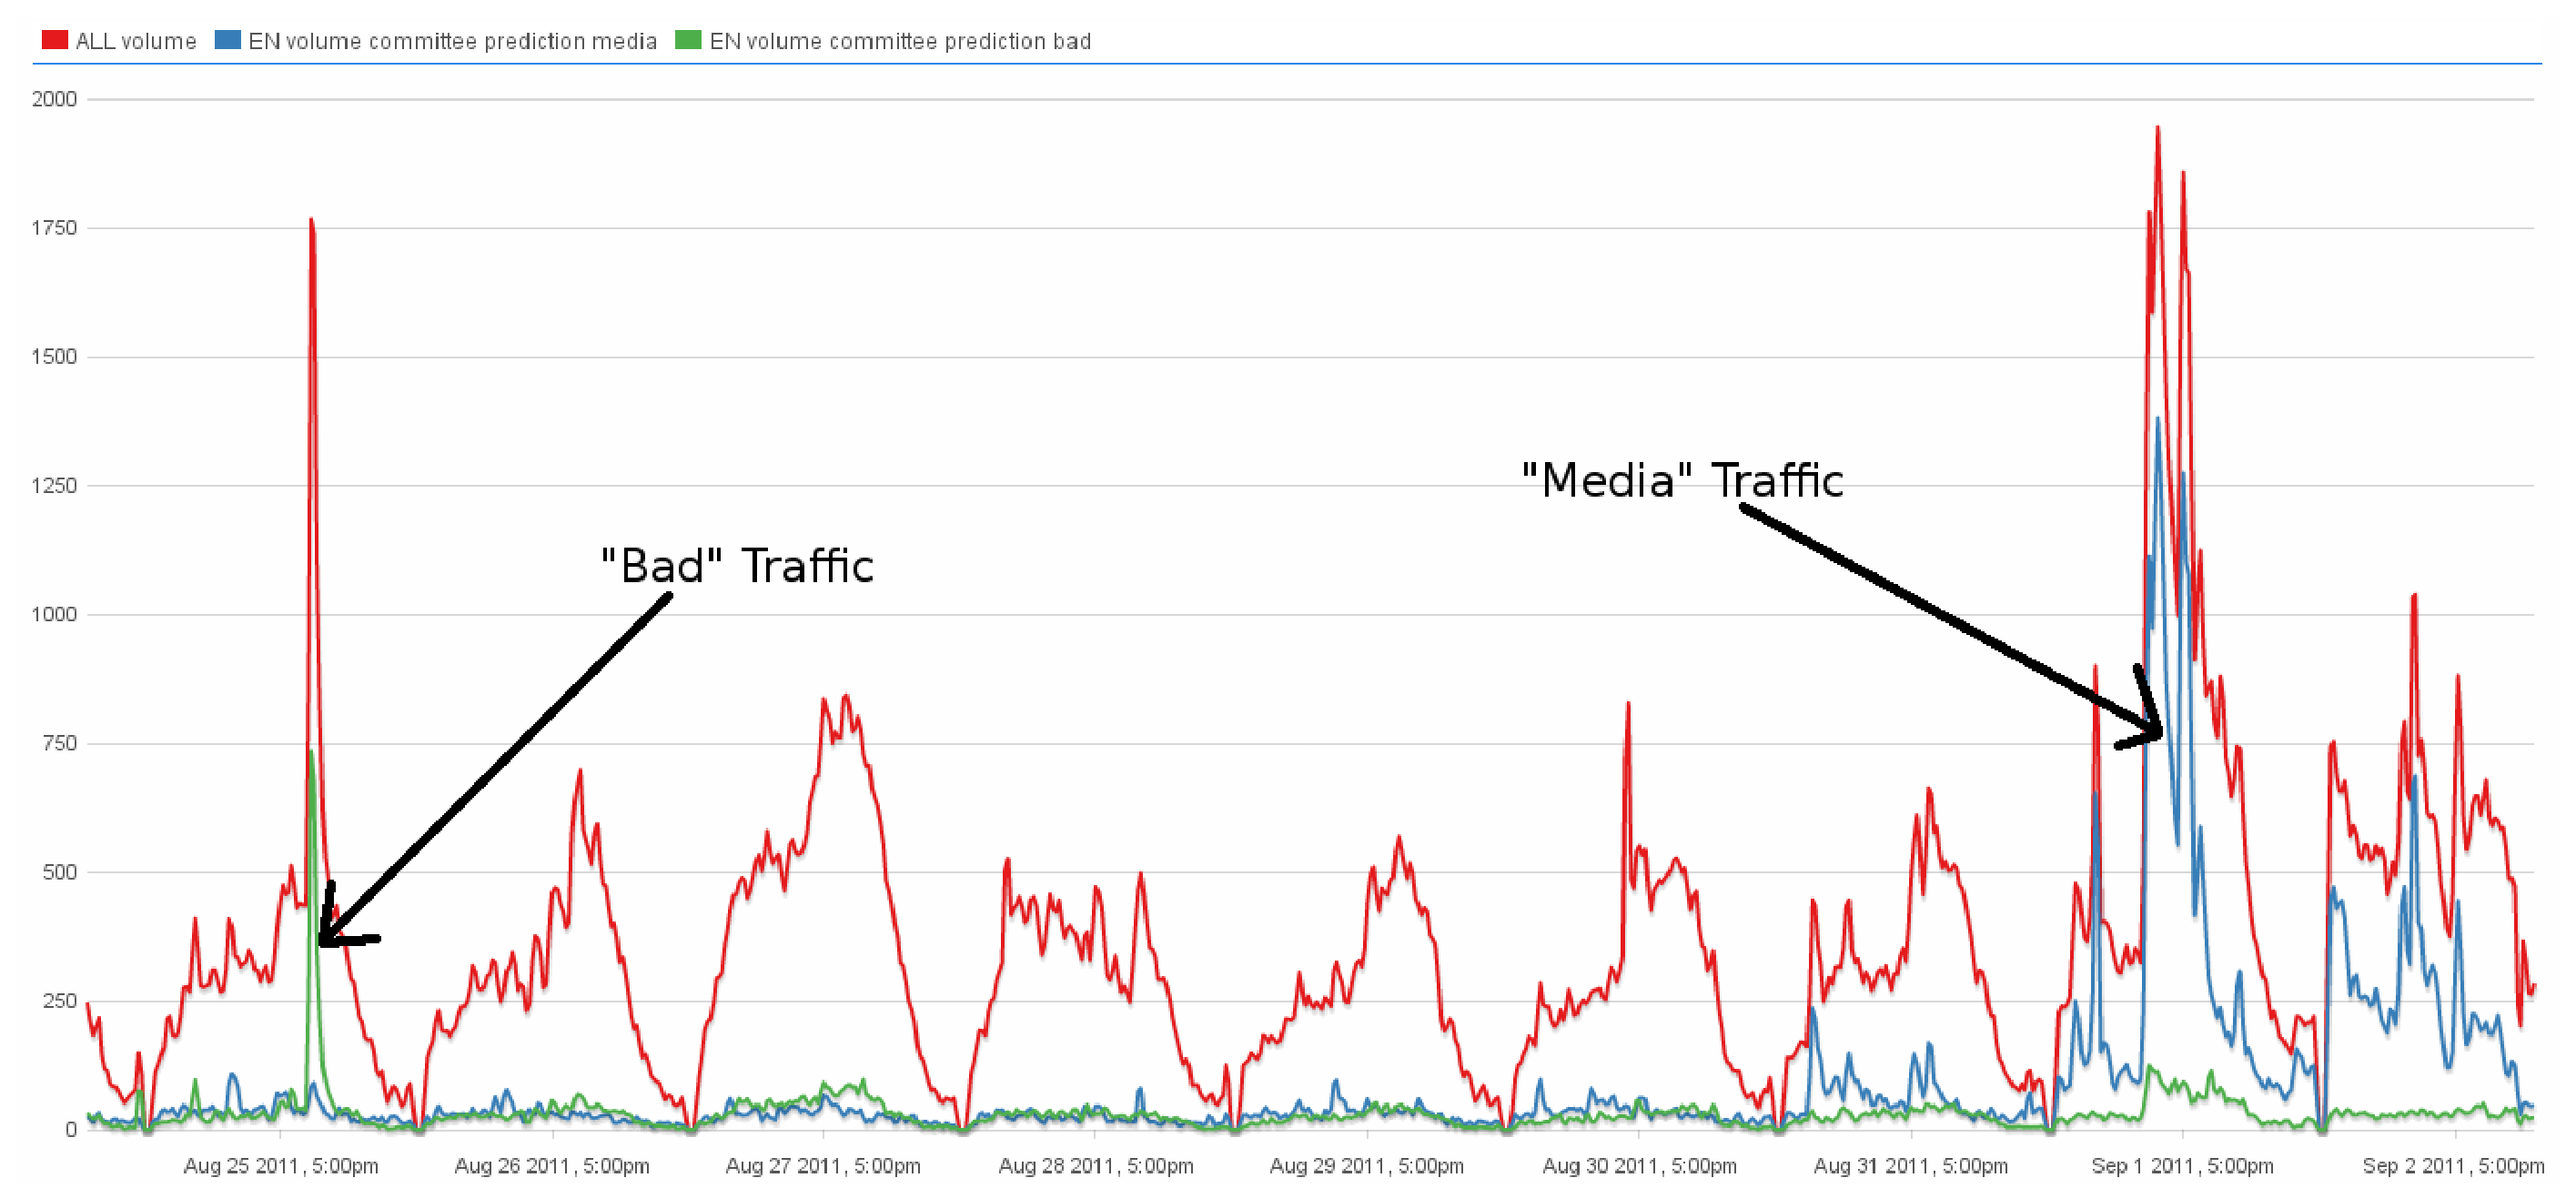
\includegraphics[width=0.8\textwidth]{images/Classified_Traffic.eps}
      \captionfonts
      \caption[Classified Traffic]{The same traffic shown in Figure~\ref{fig:anomalous-traffic}, with two addition lines: the volume of tweets classified as ``Bad'' and the volume of tweets classified as ``Media''.}
      \label{fig:classified-traffic}
   \end{center}
\end{figure}

\chapter{Classification Roadmap}
\label{class-roadmap}
The steps that SPOONS takes to use classification to detect service outages is as follows:

\begin{enumerate}
   \item Observe Netflix-related Twitter traffic and observe the different classes that the tweets fall into.
   \item Build a training set biasing anomalous traffic.
   \item Classify incoming tweets.
   \item Group classified tweets according to the type of traffic that class produces.
   \item Establish the best classifiers.
   \item Use the best classifiers in an Analysis Pipeline.
   \item Observe the differences between the total traffic and the classified traffic.
   \item Declare an outage when the two traffics diverge significantly.
\end{enumerate}

\chapter{Fitting Into The SPOONS Framework}
\label{class-framework}
Although the classifiers can be used at any stage in an analysis pipeline, the classifiers are usually implemented as
a Processor. It takes in a range of tweets and produces a classification for each tweet.

\chapter{Tweet Classes}
\label{class-tweet-classes}
After observing Netflix-related Twitter traffic, it was discovered that tweets fall into at least one of nine different categories.

\begin{itemize}
  \item \texttt{Media} -- Relate to a media story about Netflix.
  \item \texttt{Snafu} -- Talk about a Netflix outage.
  \item \texttt{Complaint} -- Complain about Netflix.
  \item \texttt{Happy} -- Express joy about Netflix.
  \item \texttt{Neutral} -- Neutral observation or comment about Netflix.
  \item \texttt{Watching} -- Updates on what the user is currently watching.
  \item \texttt{Response} -- Neutral response to another user in a Netflix-related conversation.
  \item \texttt{Refuse To Rate} -- Used for tweets that we refuse to rate entirely (usually tweets that are in a different language than the training set).
  \item \texttt{Undetermined} -- This class does not exist in the wild. It is used during classification as default for all tweets that don't match any other class.
\end{itemize}

Examples of tweets with their corresponding classes are shown in Table~\ref{table:classes}.

\begin{table}
   \begin{center}
      \begin{tabular}{|l|p{12cm}|}
         \hline
            Class & Tweet Example
         \tabularnewline\hline
            \texttt{Media} & Netflix Now Available Through Facebook - http://bit.ly/ffpBHH - [Geeky Gadgets]
         \tabularnewline\hline
            \texttt{Snafu} & And netflix is broken. Why is this happening to me.
         \tabularnewline\hline
            \texttt{Complaint} & netflix keeps taking little things i like about the site away...Why?
         \tabularnewline\hline
            \texttt{Happy} & Netflix :)
         \tabularnewline\hline
            \texttt{Neutral} & about to download this netflix free trial
         \tabularnewline\hline
            \texttt{Watching} & Watching Family Guy on Netflix
         \tabularnewline\hline
            \texttt{Response} & @BeehiveBlog  Both good movies.  I think I'll put on the netflix list.
         \tabularnewline\hline
            \texttt{Refuse To Rate} & en serio, QUIERO pagar por algo como Netflix, DEJARME pagar
         \tabularnewline\hline
      \end{tabular}
   \end{center}
   \caption[Database Tweet Attributes]{The database attributes used to describe tweets.}
   \label{table:classes}
\end{table}

\section{Tweet Groups}
\label{class-tweet-groups}
Because the goal of SPOONS is to detect anomalous times, it is useful to collapse the nine classes into
three different groups that account for the different types of Netflix-related traffic.

\begin{itemize}
  \item \texttt{Media}: Contains only the \texttt{media} class.
  \item \texttt{Bad}: Contains both the \texttt{snafu} and \texttt{complaint} classes.
  \item \texttt{Other/Normal}: Contains all other classes.
\end{itemize}

% TODO(eriq): B/W makes description hard.

Figure \ref{fig:groups} shows the amount of Netflix-related tweets during a Netflix outage and media event.
During normal times, the \texttt{normal} traffic is responsible for the majority of the overall traffic.
However during outage and media events, we see that the \texttt{bad} and \texttt{media} dominate the respective
periods.

\begin{figure}
   \begin{center}
      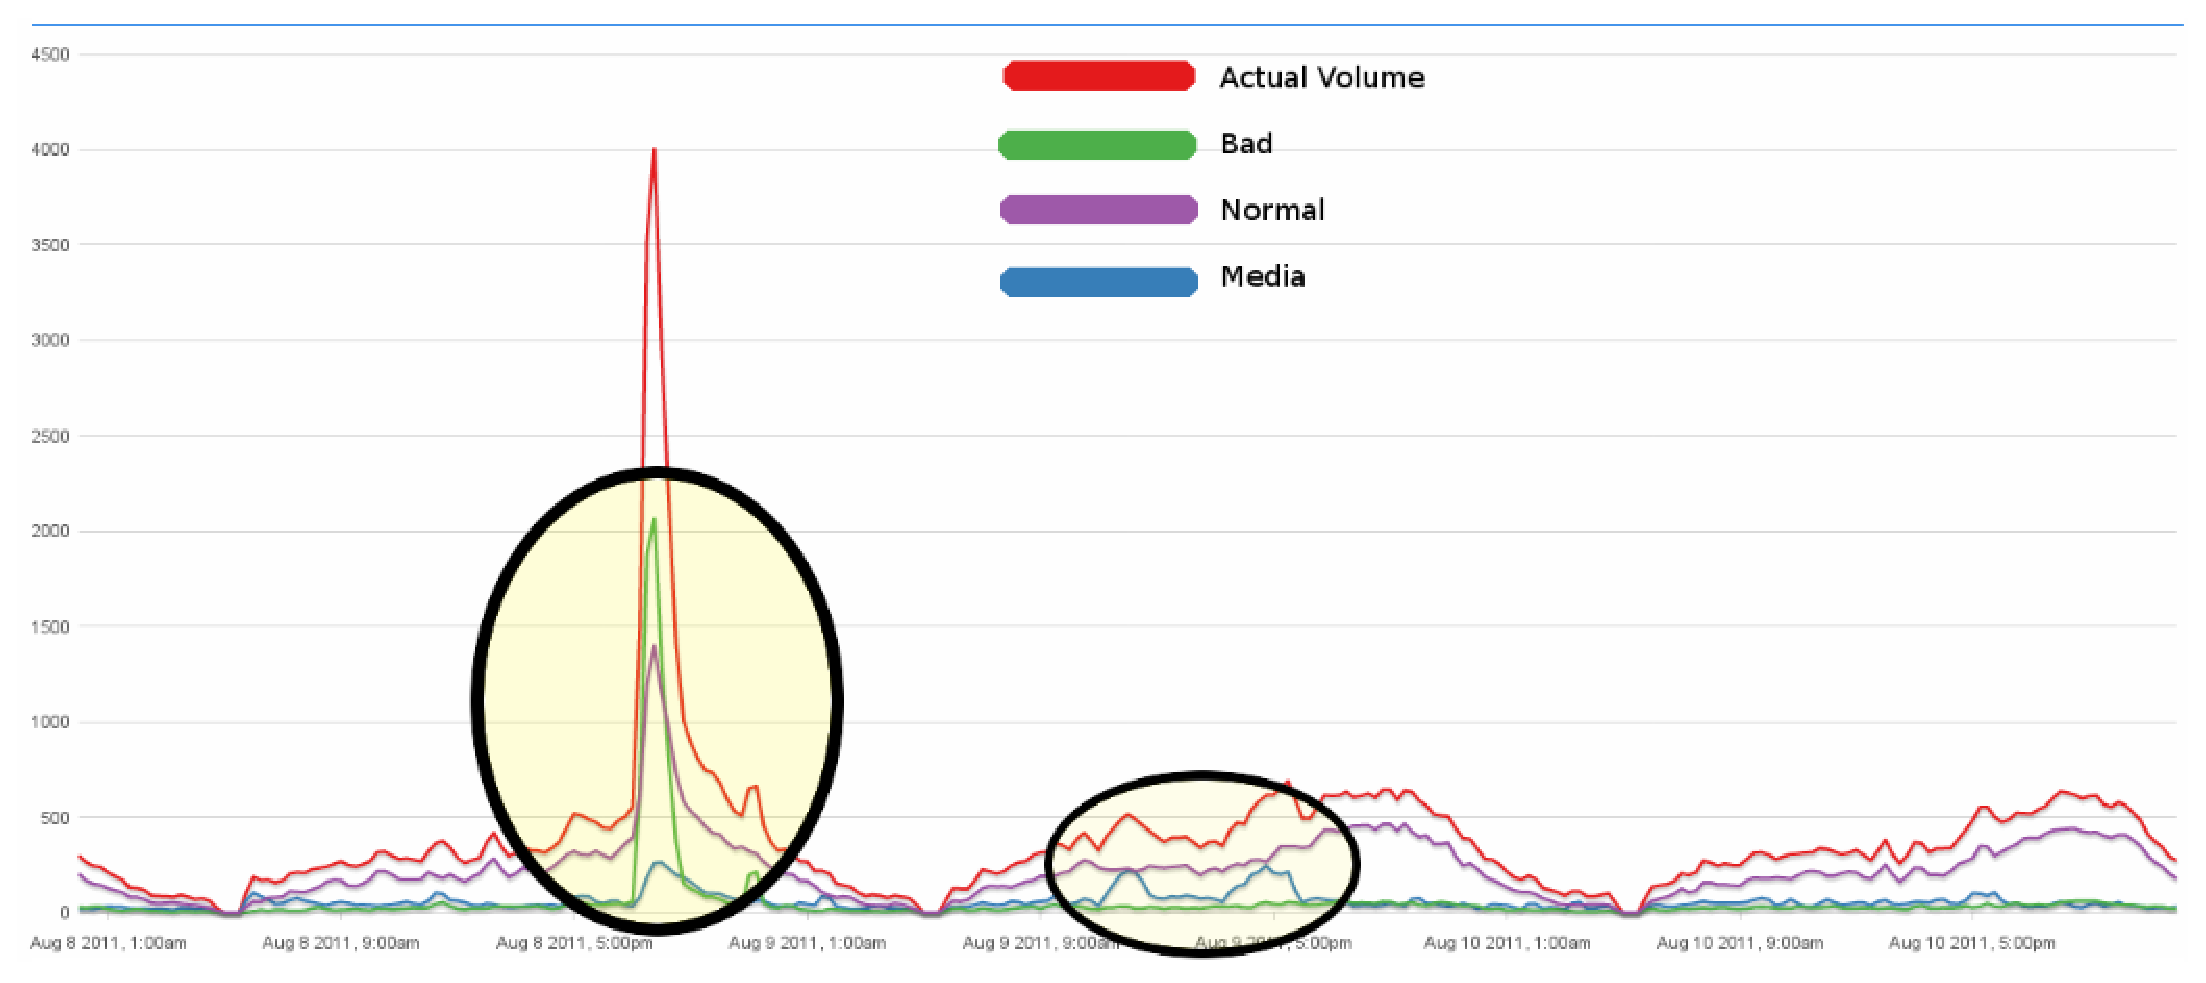
\includegraphics[width=0.8\textwidth]{images/groups.eps}
      \captionfonts
      \caption[SPOONS Groups]{The different volumes for different tweet classes during an outage (left) and media event (right).}
      \label{fig:groups}
   \end{center}
\end{figure}

\chapter{WEKA Classifiers}
\label{class-weka}
SPOONS uses several classifier from the WEKA machine learning package\cite{weka}.
All of these classifiers have been discussed in Section~\ref{background-classification-classifiers}.

\begin{itemize}
   \item Naive Bayes
   \item Bayes Net
   \item J48 (a method of generating a C4.5 decision tree\cite{j48})
   \item K-Nearest Neighbors
   \item SMO (Support Vector Machine trained with Sequential Minimal Optimization\cite{smo})
\end{itemize}

\chapter{Non-WEKA Classifiers}
\label{class-nonweka}
In addition to the WEKA classifiers, SPOONS uses two classifiers implemented from scratch.
Because of low performance and inflexible API, the WEKA classifiers are being reimplemented.
As of now, only Naive Bayes has been reimplemented. The other classifier implemented from scratch is
a BPNB classifier which is discussed in Section~\ref{background-classification-classifiers-bpnb}.

\chapter{Text Processing}
\label{class-processing}
Before the tweets are classified, they are processed. During processing, the text is transformed
to make classification of the text easier. Standard text operations like stemming, stopword removal,
and case normalization; as well as Twitter and Netflix specific operations like hashtag and movie title
recognition are preformed. After the text is processed, it is split into unigrams to be used as features
in the classifiers.

\section{Text Filtering}
\label{class-filter}
Before the input text is split into features, it goes through heavy pre-processing.
The text filtering involves normalizing the case, remove extra characters, and replacing special features.

\subsection{Link Replacement}
\label{class-filter-link-replacement}
The first step in processing the text is to replace links.
Following a link may provide information about a tweet, however the link text of the link
itself provides no information. The presence of a link, however, can provide information about
a tweet.

\subsection{Twitter Specific Symbols}
\label{class-filter-twitter-symbols}
Tweets often contain several special symbols specific to tweets.

\subsubsection{RT}
\label{class-twitter-symbols-rt}
``RT'' stands for ``re-tweet''. It means that the posted tweet is a repost of
a tweet made by another user. This symbol contains no reference to the original post.
``RT'' usually appears at the beginning of the tweet. For example, after the comedian
Conan O'Brien posted the following tweet:

\begin{center}
   If I'm ever a ghost, I hope the person I haunt has Netflix.
\end{center}

There were hundreds of identical tweets that said:

\begin{center}
   RT: If I'm ever a ghost, I hope the person I haunt has Netflix.
\end{center}

\subsubsection{\#}
\label{class-twitter-symbols-hash}
In Twitter, a ``\#'' (pronounced ``hashtag'') is a reference to some topic in Twitter.
Users can search for tweets by hashtag and see the collection of tweets supposedly about the
same topic. A hashtag does not have to reference a pre-existing topic.

\subsubsection{\@}
\label{class-twitter-symbols-at}
An ``@'' in Twitter, simply pronounced ``at'', is a reference to another Twitter user.
A reference to a user will alert that user about the posted tweet.
For example, the following tweet will reference my Twitter account.

\begin{center}
Hi there, @eriqaugustine
\end{center}

\subsection{Emoticon Parsing}
\label{class-filter-emoticon}
Emoticons are parsed out and replaced with meta words.
SPOONS emoticon parser was written by Ryan Hanarkis and Allen Dunlea as part of a project for Graduate Artificial Intelligence.
Emoticons provide a plethora of information about a tweet. Sarcasm aside,
an emoticon can surmise the sentiment of an entire tweet.

\subsection{Title Replacement}
\label{class-filter-title}
Because our tweets are always about Netflix, a television show and movie streaming service,
titles are a common occurrence. However, movie and show titles often contain words that can be
detrimental to our analysis. For example, ``Death At A Funeral'' is the title of a movie, but contains
two words that have very negative connotations: ``death'' and ``funeral''.

Without title replacement, the following tweet would be very difficult to classify:

\begin{center}
Death at a Funeral is hilarious!  \#netflix
\end{center}

However after title replacement, the tweet becomes very easy to classify:

\begin{center}
$\langle$\$title\$$\rangle$ is hilarious!  \#netflix
\end{center}

SPOONS contains a table that has over 50,000 movie and show titles on Netflix. The titles were gathered
using the Netflix API. On startup, SPOONS will build a trie (prefix tree)\cite{trie} of all of the titles. In this trie titles can
only be split on a word level, not on a character level. Therefore, moving to the next node consumes a single word.
Searching for a title becomes a simple walk down the trie.
If the walk of the trie ends on a terminal node, then a title is found. If not, then the trie is walked again from the beginning
starting at the next word in the tweet. Figure~\ref{fig:title-trie} shows a sample walk in the title trie.

\begin{figure}
   \begin{center}
      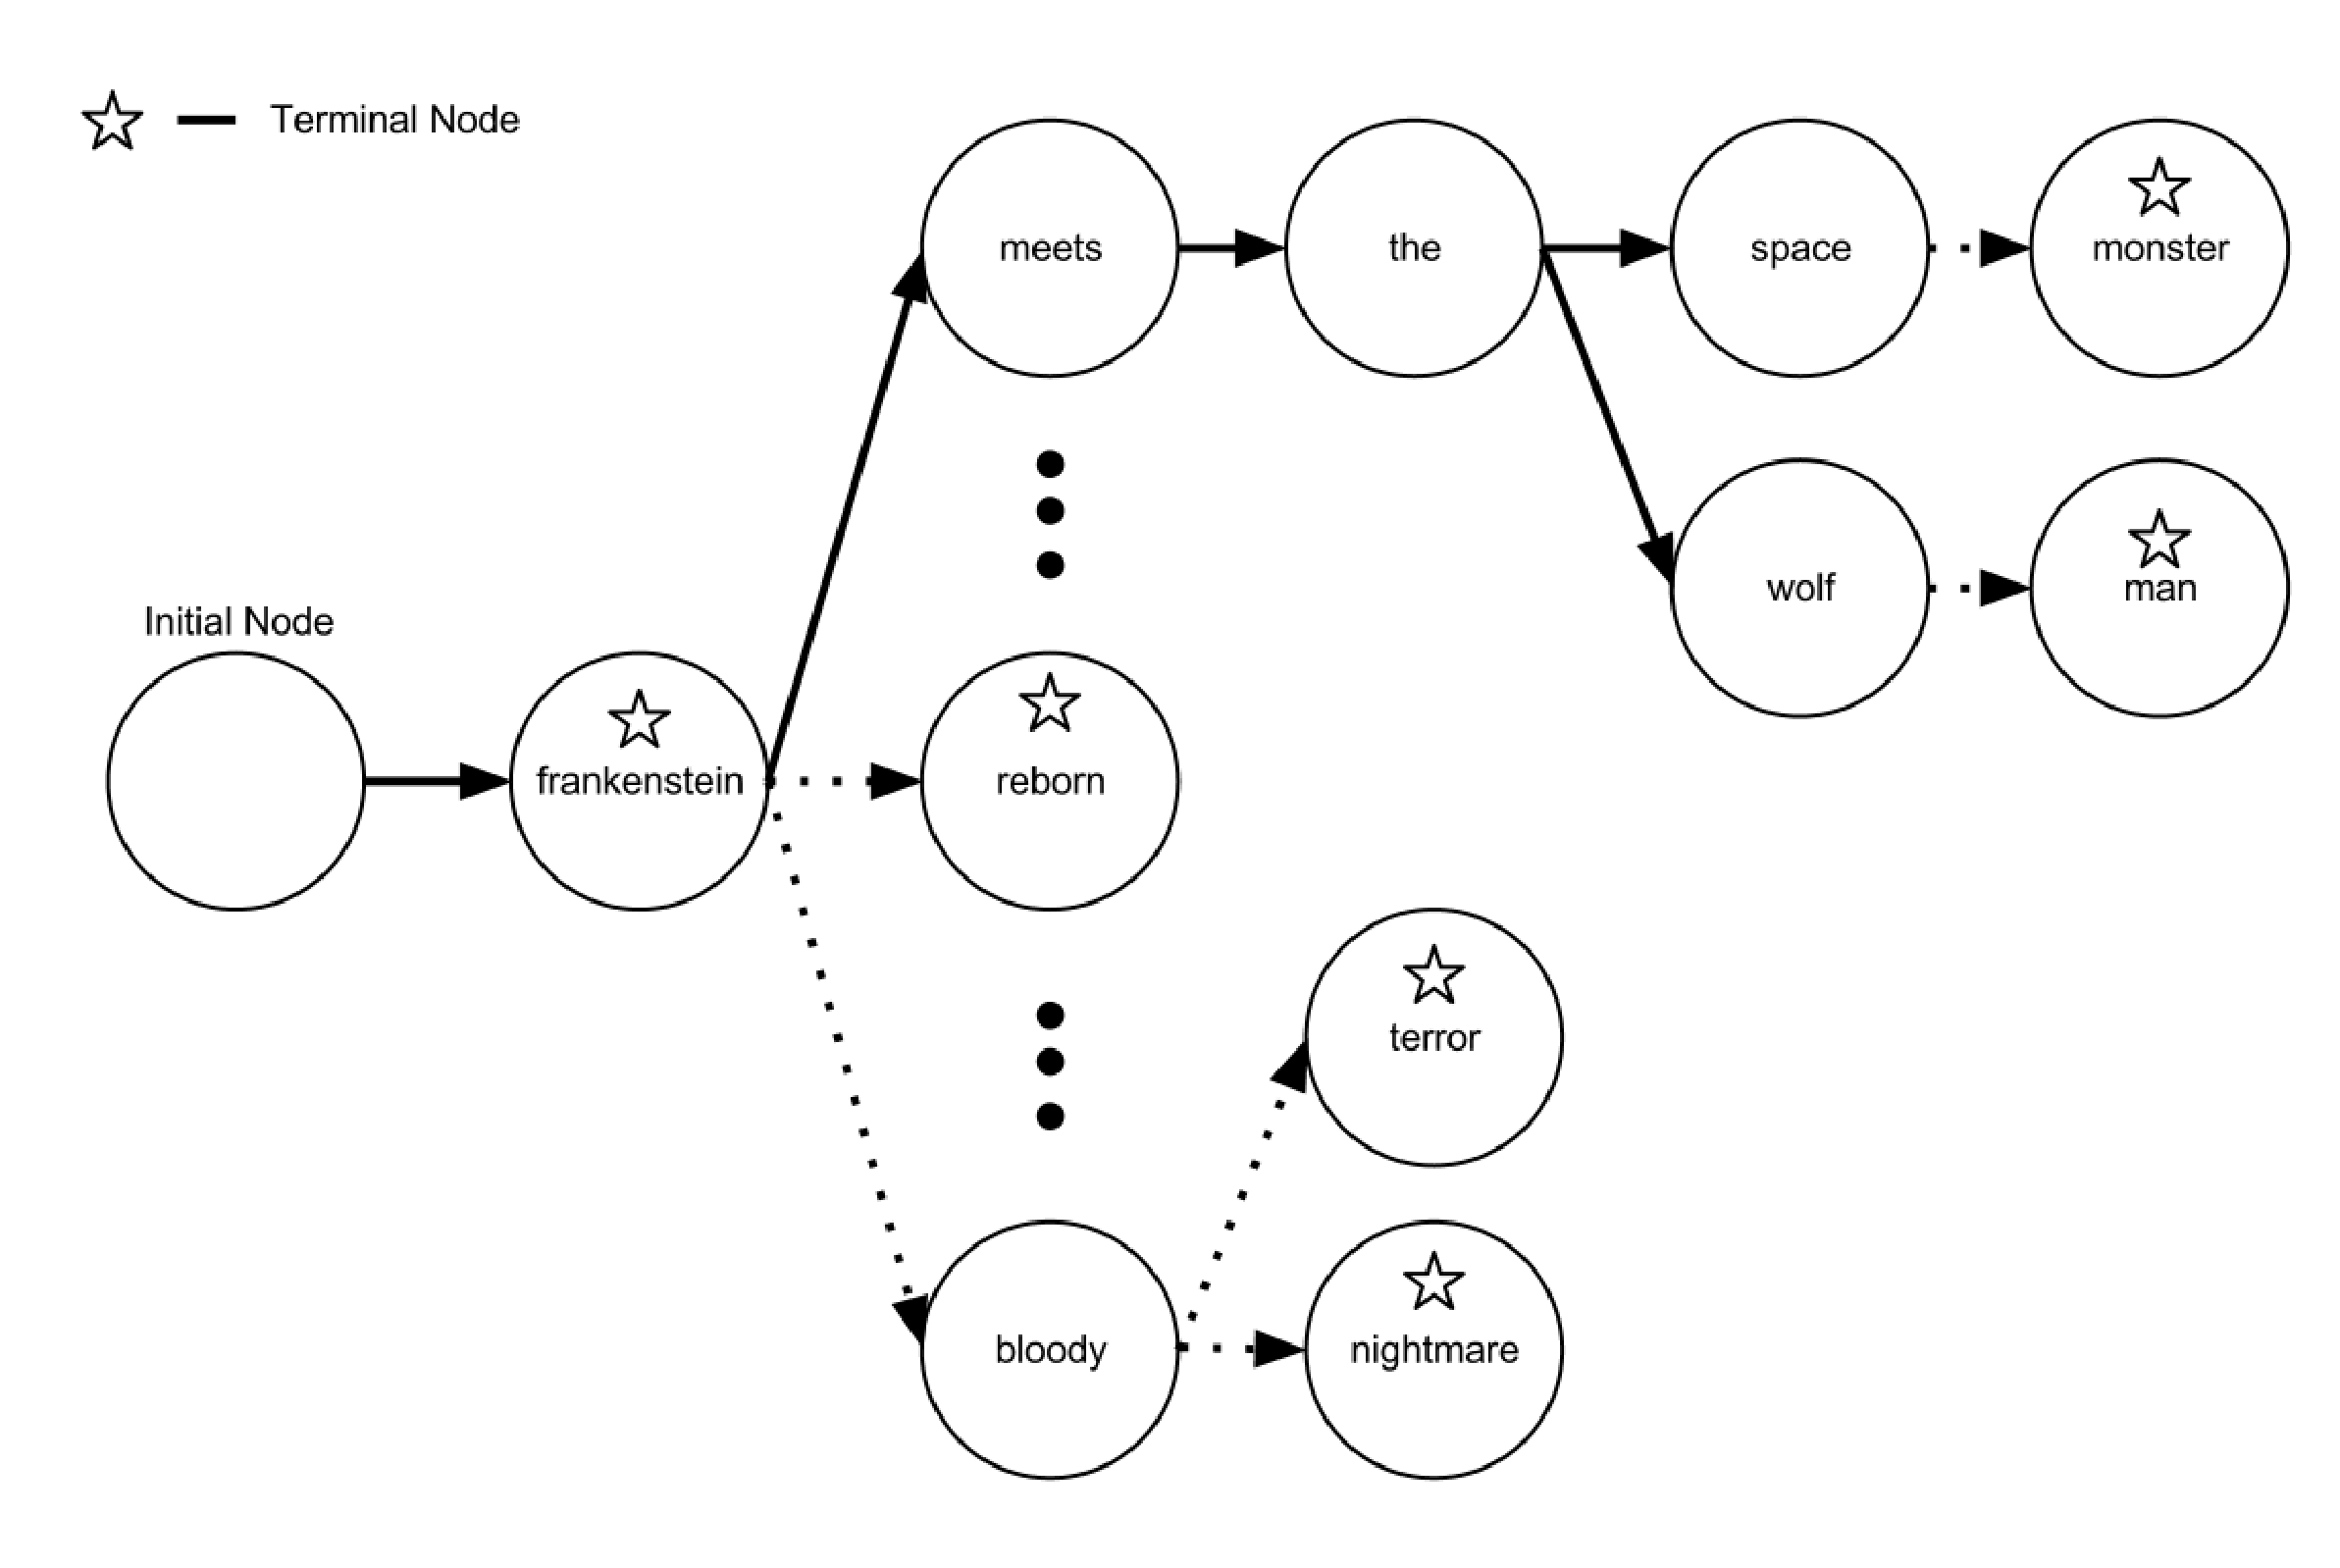
\includegraphics[width=0.8\textwidth]{images/Title_Trie.eps}
      \captionfonts
      \caption[Title Trie Walk]{A sample trie of Frankenstein movie titles. The solid lines show what nodes the search for "Frankenstein Meets The Wolf Man" would traverse.}
      \label{fig:title-trie}
   \end{center}
\end{figure}

\subsection{Stemming}
\label{class-filter-stemming}
Stemming finds the root of a word. This allows words to be categorized by their roots which
decreases the number of unique words being evaluated and emphasizes linguistic patterns.
This preprocessor uses Porter's stemmer for the English language \cite{porters}.

\subsection{Stop Word Removal}
\label{class-filter-stopword}
Stopwords, or words that carry little or no semantic information, are identified based
on a static table of words mapped to levels. Stopwords are assigned levels which allow
processes to use different sets of stop words. All words less than 3 character are also
automatically considered stop words.

\subsection{Punctuation/Non-English Character Removal}
\label{class-filter-noneng}
Removes all punctuation and
characters not in the English alphabet. This simplifies word extraction and
comparison.

\subsection{Meta Words}
\label{class-filter-meta}
Below is an overview of meta words that SPOONS recognizes:
\begin{description}
   \item[$\langle$\$link\$$\rangle$] Indicates the presence of a URL.
   \item[$\langle$\$emote:*\$$\rangle$] Replaces an emoticon.
   \item[$\langle$\$RT\$$\rangle$] Indicates that a tweet is a ``retweet'' (a repeat of another tweet).
   \item[$\langle$\$\#\$$\rangle$] Inserted when a ``hashtag'' is found in a tweet. The original subject of the hashtag is separated off into another word. E.g. ``\#Netflix'' becomes ``$\langle$\$\#\$$\rangle$ Netflix''.
   \item[$\langle$\$@\$$\rangle$] Inserted when a reference to another Twitter user is made. The user that is the subject of the reference is separated off into another word.
\end{description}

\chapter{Training Set}
\label{class-training-set}

The classifiers were trained on a small set of \textbf{759} tweets which were pulled from from periods of both normal and
anomalous traffic. Each tweet in the training set was manually classified by multiple researchers until consensus
about the classification was reached. Because the goal is anomalous traffic detection, the training set over-samples the
tweets from \texttt{media}, \texttt{snafu}, and \texttt{complaint}: categories. Table \ref{table:classCounts} documents
the structure of the training set and shows the  number of tweets classified into each of the eight categories.
Tweets were allowed to belong to multiple classes because of posts like, ``\texttt{I love netflix! Watching Law and Order
online!}'', which could be classified as both \texttt{happy} and \texttt{watching}.

\begin{table}
   \begin{center}
      \begin{tabular}{|l|c|c|c|}
         \hline
         Class  & \# Tweets & Class & \# Tweets
         \tabularnewline\hline
         \texttt{Media} & 103 & \texttt{Neutral} & 66
         \tabularnewline\hline
         \texttt{Outage} & 158  & \texttt{Watching} &  135
         \tabularnewline\hline
         \texttt{Complaint}  & 146 &  \texttt{Response} &  30
         \tabularnewline\hline
         \texttt{Happy}  & 147  & \texttt{Undetermined}  & 48
         \tabularnewline\hline
      \end{tabular}
      \caption[Netflix-related Twitter Traffic]{Overview of the Netflix-related Twitter post training set used to train classifiers in SPOONS.}
      \label{table:classCounts}
   \end{center}
\end{table}

\chapter{Evaluation}
\label{class-evaluation}
Each classifier is individually evaluated just on its ability to classify tweets against the training set.
Each classifier varied two parameters: the type of filtering and the feature selection.
The measure of accuracy is the percentage of correctly classified tweets.

Table~\ref{table:classification-summary-uncompressed} shows a summary of the results of the evaluation.
The SMO classifier took the top three spots with a top accuracy of \textbf{.5750}.
This is a decent accuracy, but much of the misclassification occurs between classes that don't matter
as much when trying to identify the different types of classes. For example, it does not matter if
a \texttt{watching} tweet is misclassified as a \texttt{happy} tweet. Both of those classes contribute to
normal background traffic. Therefore the classifiers will be evaluated again, but the different classes
will be compressed into their respective groups before the results are evaluated.

\begin{center}
   \begin{longtable}{|l|l|l|c|c|c|}
      \hline
         Classifier & Text Filter & Accuracy
      \tabularnewline\hline
         \textbf{SMOClassifier} & \textbf{None} & \textbf{0.5726}
      \tabularnewline\hline
         SMOClassifier & Full & 0.5618
      \tabularnewline\hline
         BinaryNaiveBayesClassifier & None & 0.5606
      \tabularnewline\hline
         NaiveBayesClassifier & None & 0.5462
      \tabularnewline\hline
         J48Classifier & Full & 0.5414
      \tabularnewline\hline
         BinaryNaiveBayesClassifier & Full & 0.5414
      \tabularnewline\hline
         J48Classifier & None & 0.5294
      \tabularnewline\hline
         Non-Weka BPNBClassifier & Full & 0.5210
      \tabularnewline\hline
         NaiveBayesClassifier & Full & 0.5198
      \tabularnewline\hline
         BinarySMOClassifier & Full & 0.5174
      \tabularnewline\hline
         BinarySMOClassifier & None & 0.5126
      \tabularnewline\hline
         BinaryBayesNetClassifier & Full & 0.4982
      \tabularnewline\hline
         BayesNetClassifier & None & 0.4970
      \tabularnewline\hline
         Non-Weka BPNBClassifier & None & 0.4958
      \tabularnewline\hline
         BinaryBayesNetClassifier & None & 0.4958
      \tabularnewline\hline
         BayesNetClassifier & Full & 0.4646
      \tabularnewline\hline
         BinaryJ48Classifier & Full & 0.4622
      \tabularnewline\hline
         BinaryJ48Classifier & None & 0.4514
      \tabularnewline\hline
         BinaryKNNClassifier & None & 0.4406
      \tabularnewline\hline
         KNNClassifier & None & 0.4382
      \tabularnewline\hline
         Non-Weka NaiveBayesClassifier & Full & 0.4082
      \tabularnewline\hline
         KNNClassifier & Full & 0.3854
      \tabularnewline\hline
         BinaryKNNClassifier & Full & 0.3830
      \tabularnewline\hline
         Non-Weka NaiveBayesClassifier & None & 0.3553
      \tabularnewline\hline
      \caption[Uncompressed Classification Results Summary]{Uncompressed Classification Results Summary}
      \label{table:classification-summary-uncompressed}
   \end{longtable}
\end{center}

\begin{center}
   \begin{longtable}{|l|l|l|c|c|c|}
      \hline
         Classifier & Text Filter & Accuracy
      \tabularnewline\hline
         \textbf{SMOClassifier} & \textbf{Full} & \textbf{0.8583}
      \tabularnewline\hline
         SMOClassifier & None & 0.8499
      \tabularnewline\hline
         Non-Weka BPNBClassifier & Full & 0.8271
      \tabularnewline\hline
         BinarySMOClassifier & None & 0.8259
      \tabularnewline\hline
         BinarySMOClassifier & Full & 0.8235
      \tabularnewline\hline
         BinaryNaiveBayesClassifier & None & 0.8235
      \tabularnewline\hline
         BinaryNaiveBayesClassifier & Full & 0.8199
      \tabularnewline\hline
         NaiveBayesClassifier & None & 0.8175
      \tabularnewline\hline
         Non-Weka BPNBClassifier & None & 0.8151
      \tabularnewline\hline
         J48Classifier & Full & 0.8091
      \tabularnewline\hline
         NaiveBayesClassifier & Full & 0.8079
      \tabularnewline\hline
         BinaryKNNClassifier & None & 0.7899
      \tabularnewline\hline
         J48Classifier & None & 0.7887
      \tabularnewline\hline
         KNNClassifier & None & 0.7863
      \tabularnewline\hline
         KNNClassifier & Full & 0.7623
      \tabularnewline\hline
         Non-Weka NaiveBayesClassifier & Full & 0.7611
      \tabularnewline\hline
         BinaryKNNClassifier & Full & 0.7575
      \tabularnewline\hline
         Non-Weka NaiveBayesClassifier & None & 0.7263
      \tabularnewline\hline
         BayesNetClassifier & None & 0.7263
      \tabularnewline\hline
         BinaryJ48Classifier & None & 0.6879
      \tabularnewline\hline
         BinaryBayesNetClassifier & Full & 0.6855
      \tabularnewline\hline
         BinaryBayesNetClassifier & None & 0.6819
      \tabularnewline\hline
         BinaryJ48Classifier & Full & 0.6759
      \tabularnewline\hline
         BayesNetClassifier & Full & 0.6603
      \tabularnewline\hline
      \caption[Compressed Classification Results Summary]{Compressed Classification Results Summary}
      \label{table:classification-summary-compressed}
   \end{longtable}
\end{center}



Table~\ref{table:classification-summary-compressed} shows a summary of the compressed results.
After the classes have been compressed, the SMO classifier is still on top but now with a best accuracy
of \textbf{.8583}. Compressing the classes into groups greatly increases the accuracy of the classifiers.

Full results for both the uncompressed and compressed evaluation can be found in Section~\ref{appendix-full-classifier}.

\part{Outage Detection}
\label{outage-detection}

\chapter{Ground Truth}
\label{outage-detection-truth}
Netflix has provided us with a list of outages that occurred between March 14, 2011 and January 30, 2012.
This list is not comprehensive and some of the times are questionable. Some of the outages contained in the list
are internal outages that did not affect their streaming service. These outages generated no signal on Twitter.
Therefore, errors of omission could fall into one of two categories: true failures to recognize outages, and uncatchable
outages. Regardless, we use this as our base truth about all of the Netflix outages in that time period.

\chapter{Success Metrics}
\label{outage-detection-metrics}
The accuracy of outage detection is measured using three metrics: Recall, Precision, and F$_{0.5}$.

The following definitions are used to calculate the accuracy metrics:
\begin{itemize}
   \item{tp} - True Positive. Any intersection between a reported outage range and a detected outage range.
   \item{fp} - False Positive. Any detected outage that has no intersection in the events reported by Netflix.
   \item{fn} - False Negative. An alert that has no intersection on an event reported by Netflix is a false negative.
\end{itemize}

\subsubsection{Recall}
The percent of the reported events that were caught.
\begin{center}
   $Recall = \frac{tp}{tp + fn}$
\end{center}

\subsubsection{Precision}
The percent of the alerts generated that occurred during an outage event.
Netflix has specified that a precision of 0.5 is an acceptable amount of noise.
\begin{center}
   $Precision = \frac{tp}{tp + fp}$
\end{center}

\subsubsection{F$_{0.5}$ Score}
A harmonic mean between recall and precision. The standard F$_{1}$ score evenly weighs precision and recall.
F$_{0.5}$ weighs precision more than recall. Precision is being weighed more heavily than recall because
every alert that SPOONS generates would require the intervention of a Netflix engineer. Generating too many
false positives would just cause SPOONS to be ignored.
\begin{center}
   $F_{\beta} = (1 + \beta^{2}) \cdot \frac{precision \cdot recall}{\beta^{2} \cdot precision + recall}$
\end{center}
\begin{center}
   $F_{0.5} = 1.25 \cdot \frac{precision \cdot recall}{.25 \cdot precision + recall}$
\end{center}

\chapter{Outage Detection Pipeline}
\label{outage-detection-pipeline}

\section{Processors}
\label{outage-detection-processors}

\section{Modeler}
\label{outage-detection-modeler}

\section{Monitors}
\label{outage-detection-monitors}
TODO(eriq): Describe how the different monitors will be described.
TODO(eriq): Make sure equations get numbers.

\subsection{Monitor Parameters}
\label{outage-detection-monitors-params}
TODO(eriq)
Section~\ref{arch-smoothers}
Section~\ref{arch-resistance}

\subsection{Baseline Monitor}
\label{outage-detection-monitors-Baseline}
\begin{table}[H]
   \begin{center}
      \begin{tabular}{|c|c|c|}
         \hline
            Parameter & Description & Restrictions \\
         \hline
            B & Baseline & $ B > 0 $\\
         \hline
      \end{tabular}
   \end{center}
\end{table}

\begin{table}[H]
   \begin{center}
      \begin{tabular}{|c|c|c|}
         \hline
            Input & Description & Restrictions \\
         \hline
            X & Any time series & - \\
         \hline
      \end{tabular}
   \end{center}
\end{table}

The Baseline Monitor looks for any value above B, and counts that as anomalous.
Ironically, because of its naivety it also provides a decent baseline for the Monitors.

\subsection{Windowed Standard Deviation Monitor}
\label{outage-detection-monitors-WindowStdDev}
\begin{table}[H]
   \begin{center}
      \begin{tabular}{|c|c|c|}
         \hline
            Parameter & Description & Restrictions \\
         \hline
            W & Window Size & $ W > 0 $\\
         \hline
            L & Lower Threshold & $L > 0 $\\
         \hline
            U & Upper Threshold & $U >= L $\\
         \hline
      \end{tabular}
   \end{center}
\end{table}

\begin{table}[H]
   \begin{center}
      \begin{tabular}{|c|c|c|}
         \hline
            Input & Description & Restrictions \\
         \hline
            X & Any time series & - \\
         \hline
      \end{tabular}
   \end{center}
\end{table}

The Windowed Standard Deviation Monitor is one of the simplest monitors. This monitor takes a $W$ sized window worth of data
and uses the standard deviation of the window to find outliers. Any outliers more than $L$ are considered anomalies and counts towards
an alert, but are still included in the windowed standard deviation calculation. Any value above $U$ is considered an anomaly, but not included
in the standard deviation calculation. The reason for this is that values above $U$ are extreme outliers.

The calculation for the standard deviation, is based off of an iterative approach described in Knuth's ``The Art of Computer Programming'' is used \cite{Knuth}.
Because Knuth's approach was iterative, it could be modified it to calculate for a range of values in an on-line fashion.

Adding the $k$th value, $x$, to the window:
\begin{eqnarray*}
   \lefteqn{Mean(k) = }\\
   && \frac{Mean(k - 1) * (k - 1) - Mean(k - W) + x}{k}
\end{eqnarray*}
$$
   V(k) = (x - Mean(k)) * (x - Mean(k - 1))
$$
$$
   T(k) = T(k - 1) - V(k - W) + V(k)
$$
$$
   WindowStdDev(k) = \sqrt{\frac{T(K))}{k - 1}}
$$

\subsection{Weekly Offset Windowed Standard Deviation Monitor}
\label{outage-detection-monitors-WeeklyWindowStdDev}
\begin{table}[H]
   \begin{center}
      \begin{tabular}{|c|c|c|}
         \hline
            Parameter & Description & Restrictions \\
         \hline
            W & Window Size & $ W > 0 $\\
         \hline
            L & Lower Threshold & $L > 0 $\\
         \hline 
            U & Upper Threshold & $U >= L $\\
         \hline 
      \end{tabular}
   \end{center}
\end{table}

\begin{table}[H]
   \begin{center}
      \begin{tabular}{|c|c|c|}
         \hline
            Input & Description & Restrictions \\
         \hline
            X & Any time series & - \\
         \hline
      \end{tabular}
   \end{center}
\end{table}

The Weekly Offset Window Standard Deviation Monitor leverages the periodicity of tweet volume.
Not only is there a daily pattern in traffic, but there is also an even stronger weekly pattern.
The stronger weekly pattern makes sense if one views Netflix-related Twitter traffic as a representative for the number of
people currently watching Netflix. People tend to have pattern that they follow, and people are more available
on different days of the week (especially Friday).

This monitor holds a windowed standard deviation for every 30 minute time period with 15 minute offsets
for every week. Therefore, values are not compared to the other values around it, but to expected values from
previous weeks. This monitor uses the same tactics as the Windows Standard Deviation Monitor for counting anomalies.

\subsection{Mean Squared Error Monitor}
\label{outage-detection-monitors-MSE}
\begin{table}[H]
   \begin{center}
      \begin{tabular}{|c|c|c|}
         \hline
            Parameter & Description & Restrictions \\
         \hline
            W & Window Size & $ W > 0 $\\
         \hline
            T & Threshold & $ T > 0 $\\
         \hline
      \end{tabular}
   \end{center}
\end{table}

\begin{table}[H]
   \begin{center}
      \begin{tabular}{|c|c|c|}
         \hline
            Input & Description & Restrictions \\
         \hline
            X & The expected time series & - \\
         \hline
            Y & The actual time series & $ Y(k) < X(k) $ \\
         \hline
      \end{tabular}
   \end{center}
\end{table}

The Mean square Error Monitor keeps a windowed mean squared error (MSE). This monitor requires two sets of input, a set
of expected values and a set of actual values. Any value that causes the MSE to go above a certain threshold, $T$,
counts towards an anomaly.

Adding the $k$th value to the window MSE:
$$
   V(k) = (X(k) - Y(k))^{2}
$$
\begin{eqnarray*}
   \lefteqn{MSE(k) = }\\
   && \frac{MSE(k - 1) * (k - 1) - V(k - W) + V(k)}{k}
\end{eqnarray*}

\subsection{Ratio Monitor}
\label{outage-detection-monitors-Ratio}
\begin{table}[H]
   \begin{center}
      \begin{tabular}{|c|c|c|}
         \hline
            Parameter & Description & Restrictions \\
         \hline
            T & Threshold & $ 0 < T < 1 $\\
         \hline
      \end{tabular}
   \end{center}
\end{table}

\begin{table}[H]
   \begin{center}
      \begin{tabular}{|c|c|c|}
         \hline
            Input & Description & Restrictions \\
         \hline
            X & The expected time series & - \\
         \hline
            Y & The actual time series & $ Y(k) < X(k) $\\
         \hline
      \end{tabular}
   \end{center}
\end{table}

The Ratio Monitor takes the ratio of the actual value over the expected value for every time period.
Whenever the ratio dips under the threshold $T$, then that period counts towards an anomaly.
This monitor may seem simple, but the real challenge lies in picking a proper $X$ and $Y$.
If a good approximating time series can be chosen, then the monitor can be very successful.

\subsection{Class Correlation Monitor}
\label{outage-detection-monitors-Correlation}
\begin{table}[H]
   \begin{center}
      \begin{tabular}{|c|c|c|}
         \hline
            Parameter & Description & Restrictions \\
         \hline
            W & Window Size & $ W > 0 $\\
         \hline
            T & Threshold & $ -1 < T < 1 $\\
         \hline
      \end{tabular}
   \end{center}
\end{table}

\begin{table}[H]
   \begin{center}
      \begin{tabular}{|c|c|c|}
         \hline
            Input & Description & Restrictions \\
         \hline
            X & The expected time series & - \\
         \hline
            Y & The actual time series & $ Y(k) < X(k) $\\
         \hline
      \end{tabular}
   \end{center}
\end{table}

The Correlation Monitor takes the Pearson Correlation between $X$ and $Y$ for a running window of size $W$.
Pearson Correlation is used because of its ability to catch the linear correlation between two time series within
a normalized range.

For performance reasons SPOONS uses an approximation of Pearson Correlation which uses the windowed standard deviation approach
described in Section~\ref{outage-detection-monitors-WindowStdDev}.

Adding the $k$th value, to the window:
$$
   Let \bar{X} be the windowed mean of X.
$$
$$
   Let \bar{Y} be the windowed mean of Y.
$$
\begin{eqnarray*}
   \lefteqn{T(k) = }\\
   && T(k - 1) + (X(k) * Y(k)) - (X(k - W) * Y(k -W))
\end{eqnarray*}
\begin{eqnarray*}
   \lefteqn{Pearson(k) = }\\
   && \frac{T(k) - (W * \bar{X} * \bar{Y})}{(W - 1) * WindowStdDev(X) * WindowStdDev(Y)}
\end{eqnarray*}

\chapter{Results}
\label{outage-detection-results}
TODO(eriq): Numbers

\part{Conclusions}
\label{conclusions}
TODO(eriq)

\chapter{Current Limitations of SPOONS}
\label{limitations}
TODO(eriq)
Severity
Nature of Outage
Malicious Tweet Attack
Know What To Search For (dynamic search generation)

\chapter{Current and Future Work}
\label{future-work}

\section{WEKA Classifier Reimplementation}
\label{future-work-weka}
The WEKA machine learning package offers a wide variety of classifiers.
However, their implementation and API has some room for improvement.
Because of this, SPOONS already uses two classifiers implemented from scratch.
I plan on continuing this to make a classification package centered around performance
and ease of use.

\section{Advanced Sentiment Analysis}
\label{future-work-kim}
Kim Paterson, a member of the SPOONS team, is currently working on improving the sentiment
analysis work from Cailin Cushing\cite{cailinThesis}. If completed, then SPOONS can use
both text classification and sentiment analysis to determine when there is an outage.
Because of their orthogonal natures, having both would allow SPOONS to recognize even more outages.

\section{SPOONS Scaling}
\label{future-work-brett}
Another member of the SPOONS team, Brett Armstrong, is working to improve the scalability of SPOONS.
Because of its distributed architecture (see Section~\ref{arch-dist}), SPOONS already has the potential to
scale horizontally. If there is too much traffic/work, then another server can just be added to the cluster.
However, that currently requires manual intervention. Since there are spikes when outages occur, we may not know
when there is going to be a lot of traffic. To solve this problem, Brett will use SPOONS to monitor itself.
The end result of an Analysis Pipeline will not be an email alert, rather it will be the creation of a new
AWS instance.

% ------------- End main chapters ----------------------

\appendix
\chapter{SPOONS Database Schema Highlights}
\label{appendix-db-schema}

\section{DATA\_tweets}
\begin{lstlisting}
CREATE TABLE DATA_tweets (
   twitter_id varchar(32) COLLATE utf8_unicode_ci NOT NULL,
   published int(11) NOT NULL,
   content text COLLATE utf8_unicode_ci NOT NULL,
   source text COLLATE utf8_unicode_ci,
   lang varchar(3) COLLATE utf8_unicode_ci NOT NULL,
   author varchar(50) COLLATE utf8_unicode_ci NOT NULL DEFAULT 'Jon Doe',
   frame_id int(11) DEFAULT NULL,
   id int(11) NOT NULL AUTO_INCREMENT,
   place text COLLATE utf8_unicode_ci,
   geo text COLLATE utf8_unicode_ci,
   PRIMARY KEY (id),
   UNIQUE KEY tweet_id (twitter_id),
   UNIQUE KEY twitter_id (twitter_id),
   KEY frame_index (frame_id),
   KEY published_index (published),
   KEY lang (lang)
);
\end{lstlisting}

\chapter{Full Classifier Evaluation Results}
\label{appendix-full-classifier}
\begin{table}[ht]
\footnotesize
\begin{center}
\subfloat[Non-Weka NaiveBayesClassifier][Non-Weka NaiveBayesClassifier]{
\scalebox{0.53}{
\begin{tabular}{|c|c|c|c|c|c|c|c|c|c|}
\hline
   \diaghead{\theadfont Diag ColumnmnHead II}{Classified}{Actual} & undecided & media & neutral & snafu & watching & response & complaint & refuse to rate & happy \\
\hline
   undecided & \textbf{0} & 0 & 0 & 0 & 0 & 0 & 0 & 0 & 0 \\
\hline
   media & 0 & \textbf{48} & 1 & 0 & 2 & 2 & 0 & 2 & 2 \\
\hline
   neutral & 0 & 50 & \textbf{40} & 48 & 65 & 11 & 41 & 24 & 40 \\
\hline
   snafu & 0 & 0 & 3 & \textbf{69} & 3 & 4 & 53 & 0 & 36 \\
\hline
   watching & 0 & 1 & 8 & 3 & \textbf{46} & 6 & 4 & 2 & 22 \\
\hline
   response & 0 & 2 & 8 & 6 & 6 & \textbf{1} & 1 & 2 & 8 \\
\hline
   complaint & 0 & 2 & 2 & 32 & 3 & 0 & \textbf{44} & 0 & 7 \\
\hline
   refuse to rate & 0 & 0 & 0 & 0 & 1 & 1 & 0 & \textbf{18} & 2 \\
\hline
   happy & 0 & 0 & 4 & 0 & 9 & 5 & 3 & 0 & \textbf{30} \\
\hline
\end{tabular}
}
}

\subfloat[Non-Weka BPNBClassifier][Non-Weka BPNBClassifier]{
\scalebox{0.53}{
\begin{tabular}{|c|c|c|c|c|c|c|c|c|c|}
\hline
   \diaghead{\theadfont Diag ColumnmnHead II}{Classified}{Actual} & undecided & media & neutral & snafu & watching & response & complaint & refuse to rate & happy \\
\hline
   undecided & \textbf{0} & 0 & 0 & 0 & 0 & 0 & 0 & 0 & 0 \\
\hline
   media & 0 & \textbf{93} & 9 & 0 & 4 & 3 & 6 & 9 & 4 \\
\hline
   neutral & 0 & 1 & \textbf{12} & 2 & 23 & 7 & 3 & 2 & 17 \\
\hline
   snafu & 0 & 1 & 5 & \textbf{104} & 5 & 4 & 66 & 0 & 41 \\
\hline
   watching & 0 & 1 & 16 & 10 & \textbf{83} & 9 & 6 & 2 & 32 \\
\hline
   response & 0 & 3 & 13 & 5 & 7 & \textbf{0} & 3 & 2 & 6 \\
\hline
   complaint & 0 & 3 & 4 & 34 & 2 & 0 & \textbf{57} & 1 & 10 \\
\hline
   refuse to rate & 0 & 1 & 0 & 1 & 1 & 1 & 0 & \textbf{29} & 2 \\
\hline
   happy & 0 & 0 & 7 & 2 & 10 & 6 & 5 & 3 & \textbf{35} \\
\hline
\end{tabular}
}
}

\subfloat[NaiveBayesClassifier][NaiveBayesClassifier]{
\scalebox{0.53}{
\begin{tabular}{|c|c|c|c|c|c|c|c|c|c|}
\hline
   \diaghead{\theadfont Diag ColumnmnHead II}{Classified}{Actual} & undecided & media & neutral & snafu & watching & response & complaint & refuse to rate & happy \\
\hline
   undecided & \textbf{0} & 0 & 0 & 0 & 0 & 0 & 0 & 0 & 0 \\
\hline
   media & 0 & \textbf{85} & 0 & 0 & 0 & 2 & 1 & 6 & 1 \\
\hline
   neutral & 0 & 4 & \textbf{25} & 6 & 26 & 14 & 12 & 4 & 22 \\
\hline
   snafu & 0 & 1 & 3 & \textbf{94} & 2 & 3 & 42 & 0 & 15 \\
\hline
   watching & 0 & 2 & 11 & 7 & \textbf{82} & 6 & 8 & 1 & 14 \\
\hline
   response & 0 & 4 & 13 & 7 & 9 & \textbf{3} & 10 & 2 & 6 \\
\hline
   complaint & 0 & 0 & 3 & 25 & 1 & 0 & \textbf{54} & 2 & 7 \\
\hline
   refuse to rate & 0 & 6 & 0 & 1 & 0 & 0 & 0 & \textbf{30} & 0 \\
\hline
   happy & 0 & 1 & 11 & 18 & 15 & 2 & 19 & 3 & \textbf{82} \\
\hline
\end{tabular}
}
}

\subfloat[BayesNetClassifier][BayesNetClassifier]{
\scalebox{0.53}{
\begin{tabular}{|c|c|c|c|c|c|c|c|c|c|}
\hline
   \diaghead{\theadfont Diag ColumnmnHead II}{Classified}{Actual} & undecided & media & neutral & snafu & watching & response & complaint & refuse to rate & happy \\
\hline
   undecided & \textbf{0} & 0 & 0 & 0 & 0 & 0 & 0 & 0 & 0 \\
\hline
   media & 0 & \textbf{87} & 1 & 0 & 0 & 2 & 2 & 9 & 1 \\
\hline
   neutral & 0 & 4 & \textbf{1} & 0 & 0 & 0 & 0 & 1 & 0 \\
\hline
   snafu & 0 & 0 & 9 & \textbf{77} & 6 & 4 & 36 & 2 & 26 \\
\hline
   watching & 0 & 2 & 20 & 9 & \textbf{105} & 9 & 10 & 0 & 21 \\
\hline
   response & 0 & 0 & 0 & 0 & 1 & \textbf{0} & 0 & 0 & 0 \\
\hline
   complaint & 0 & 1 & 1 & 21 & 1 & 1 & \textbf{24} & 1 & 2 \\
\hline
   refuse to rate & 0 & 8 & 2 & 0 & 0 & 0 & 0 & \textbf{23} & 0 \\
\hline
   happy & 0 & 1 & 32 & 51 & 22 & 14 & 74 & 12 & \textbf{97} \\
\hline
\end{tabular}
}
}

\caption{Uncompressed, None Filter Classification Confusion Matrices}
\end{center}
\end{table}
\begin{table}[ht]
\ContinuedFloat
\footnotesize
\begin{center}
\subfloat[J48Classifier][J48Classifier]{
\scalebox{0.53}{
\begin{tabular}{|c|c|c|c|c|c|c|c|c|c|}
\hline
   \diaghead{\theadfont Diag ColumnmnHead II}{Classified}{Actual} & undecided & media & neutral & snafu & watching & response & complaint & refuse to rate & happy \\
\hline
   undecided & \textbf{0} & 0 & 0 & 0 & 0 & 0 & 0 & 0 & 0 \\
\hline
   media & 0 & \textbf{95} & 4 & 0 & 2 & 2 & 2 & 11 & 1 \\
\hline
   neutral & 0 & 1 & \textbf{9} & 5 & 6 & 6 & 4 & 2 & 5 \\
\hline
   snafu & 0 & 0 & 5 & \textbf{84} & 2 & 5 & 37 & 4 & 9 \\
\hline
   watching & 0 & 2 & 13 & 3 & \textbf{84} & 5 & 5 & 0 & 17 \\
\hline
   response & 0 & 0 & 1 & 0 & 5 & \textbf{0} & 1 & 1 & 5 \\
\hline
   complaint & 0 & 1 & 7 & 36 & 7 & 1 & \textbf{54} & 6 & 9 \\
\hline
   refuse to rate & 0 & 3 & 3 & 2 & 0 & 0 & 4 & \textbf{14} & 0 \\
\hline
   happy & 0 & 1 & 24 & 28 & 29 & 11 & 39 & 10 & \textbf{101} \\
\hline
\end{tabular}
}
}

\subfloat[KNNClassifier][KNNClassifier]{
\scalebox{0.53}{
\begin{tabular}{|c|c|c|c|c|c|c|c|c|c|}
\hline
   \diaghead{\theadfont Diag ColumnmnHead II}{Classified}{Actual} & undecided & media & neutral & snafu & watching & response & complaint & refuse to rate & happy \\
\hline
   undecided & \textbf{0} & 0 & 0 & 0 & 0 & 0 & 0 & 0 & 0 \\
\hline
   media & 0 & \textbf{56} & 0 & 0 & 1 & 2 & 0 & 2 & 0 \\
\hline
   neutral & 0 & 0 & \textbf{3} & 0 & 10 & 4 & 4 & 0 & 3 \\
\hline
   snafu & 0 & 0 & 2 & \textbf{45} & 0 & 4 & 36 & 0 & 1 \\
\hline
   watching & 0 & 1 & 7 & 0 & \textbf{73} & 5 & 2 & 1 & 10 \\
\hline
   response & 0 & 2 & 4 & 4 & 4 & \textbf{0} & 0 & 1 & 5 \\
\hline
   complaint & 0 & 0 & 5 & 59 & 5 & 1 & \textbf{61} & 0 & 5 \\
\hline
   refuse to rate & 0 & 0 & 0 & 0 & 0 & 1 & 0 & \textbf{4} & 0 \\
\hline
   happy & 0 & 44 & 45 & 50 & 42 & 13 & 43 & 40 & \textbf{123} \\
\hline
\end{tabular}
}
}

\subfloat[SMOClassifier][SMOClassifier]{
\scalebox{0.53}{
\begin{tabular}{|c|c|c|c|c|c|c|c|c|c|}
\hline
   \diaghead{\theadfont Diag ColumnmnHead II}{Classified}{Actual} & undecided & media & neutral & snafu & watching & response & complaint & refuse to rate & happy \\
\hline
   undecided & \textbf{0} & 0 & 0 & 0 & 0 & 0 & 0 & 0 & 0 \\
\hline
   media & 0 & \textbf{98} & 3 & 0 & 2 & 2 & 2 & 9 & 1 \\
\hline
   neutral & 0 & 0 & \textbf{11} & 1 & 12 & 5 & 5 & 1 & 9 \\
\hline
   snafu & 0 & 0 & 2 & \textbf{87} & 3 & 4 & 40 & 1 & 3 \\
\hline
   watching & 0 & 2 & 16 & 4 & \textbf{88} & 7 & 4 & 1 & 13 \\
\hline
   response & 0 & 2 & 7 & 4 & 5 & \textbf{0} & 1 & 1 & 6 \\
\hline
   complaint & 0 & 0 & 7 & 41 & 4 & 3 & \textbf{68} & 0 & 8 \\
\hline
   refuse to rate & 0 & 0 & 0 & 0 & 0 & 1 & 1 & \textbf{18} & 0 \\
\hline
   happy & 0 & 1 & 20 & 21 & 21 & 8 & 25 & 17 & \textbf{107} \\
\hline
\end{tabular}
}
}

\subfloat[BinaryNaiveBayesClassifier][BinaryNaiveBayesClassifier]{
\scalebox{0.53}{
\begin{tabular}{|c|c|c|c|c|c|c|c|c|c|}
\hline
   \diaghead{\theadfont Diag ColumnmnHead II}{Classified}{Actual} & undecided & media & neutral & snafu & watching & response & complaint & refuse to rate & happy \\
\hline
   undecided & \textbf{0} & 0 & 0 & 0 & 0 & 0 & 0 & 0 & 0 \\
\hline
   media & 0 & \textbf{98} & 1 & 0 & 0 & 2 & 1 & 13 & 1 \\
\hline
   neutral & 0 & 1 & \textbf{23} & 6 & 21 & 14 & 11 & 4 & 17 \\
\hline
   snafu & 0 & 0 & 2 & \textbf{97} & 2 & 3 & 45 & 1 & 17 \\
\hline
   watching & 0 & 2 & 12 & 7 & \textbf{92} & 6 & 10 & 0 & 19 \\
\hline
   response & 0 & 2 & 13 & 7 & 5 & \textbf{3} & 8 & 3 & 6 \\
\hline
   complaint & 0 & 0 & 4 & 25 & 2 & 0 & \textbf{53} & 1 & 9 \\
\hline
   refuse to rate & 0 & 0 & 0 & 1 & 0 & 0 & 0 & \textbf{23} & 0 \\
\hline
   happy & 0 & 0 & 11 & 15 & 13 & 2 & 18 & 3 & \textbf{78} \\
\hline
\end{tabular}
}
}

\caption{Uncompressed, None Filter Classification Confusion Matrices Cont.}
\end{center}
\end{table}
\begin{table}[ht]
\ContinuedFloat
\footnotesize
\begin{center}
\subfloat[BinaryJ48Classifier][BinaryJ48Classifier]{
\scalebox{0.53}{
\begin{tabular}{|c|c|c|c|c|c|c|c|c|c|}
\hline
   \diaghead{\theadfont Diag ColumnmnHead II}{Classified}{Actual} & undecided & media & neutral & snafu & watching & response & complaint & refuse to rate & happy \\
\hline
   undecided & \textbf{0} & 0 & 0 & 0 & 0 & 0 & 0 & 0 & 0 \\
\hline
   media & 0 & \textbf{97} & 2 & 0 & 1 & 2 & 2 & 14 & 1 \\
\hline
   neutral & 0 & 0 & \textbf{4} & 0 & 4 & 2 & 1 & 0 & 3 \\
\hline
   snafu & 0 & 2 & 10 & \textbf{61} & 6 & 4 & 30 & 2 & 20 \\
\hline
   watching & 0 & 0 & 10 & 6 & \textbf{80} & 4 & 5 & 1 & 11 \\
\hline
   response & 0 & 0 & 0 & 0 & 0 & \textbf{0} & 0 & 0 & 0 \\
\hline
   complaint & 0 & 1 & 3 & 26 & 13 & 1 & \textbf{41} & 5 & 24 \\
\hline
   refuse to rate & 0 & 2 & 1 & 0 & 0 & 0 & 0 & \textbf{5} & 0 \\
\hline
   happy & 0 & 1 & 36 & 65 & 31 & 17 & 67 & 21 & \textbf{88} \\
\hline
\end{tabular}
}
}

\subfloat[BinaryBayesNetClassifier][BinaryBayesNetClassifier]{
\scalebox{0.53}{
\begin{tabular}{|c|c|c|c|c|c|c|c|c|c|}
\hline
   \diaghead{\theadfont Diag ColumnmnHead II}{Classified}{Actual} & undecided & media & neutral & snafu & watching & response & complaint & refuse to rate & happy \\
\hline
   undecided & \textbf{0} & 0 & 0 & 0 & 0 & 0 & 0 & 0 & 0 \\
\hline
   media & 0 & \textbf{90} & 2 & 0 & 0 & 2 & 1 & 10 & 1 \\
\hline
   neutral & 0 & 10 & \textbf{2} & 1 & 1 & 1 & 2 & 2 & 2 \\
\hline
   snafu & 0 & 0 & 9 & \textbf{85} & 4 & 4 & 33 & 2 & 26 \\
\hline
   watching & 0 & 2 & 18 & 6 & \textbf{107} & 9 & 10 & 0 & 19 \\
\hline
   response & 0 & 0 & 0 & 0 & 0 & \textbf{0} & 0 & 0 & 0 \\
\hline
   complaint & 0 & 0 & 32 & 64 & 20 & 14 & \textbf{99} & 12 & 91 \\
\hline
   refuse to rate & 0 & 1 & 0 & 2 & 0 & 0 & 0 & \textbf{22} & 0 \\
\hline
   happy & 0 & 0 & 3 & 0 & 3 & 0 & 1 & 0 & \textbf{8} \\
\hline
\end{tabular}
}
}

\subfloat[BinaryKNNClassifier][BinaryKNNClassifier]{
\scalebox{0.53}{
\begin{tabular}{|c|c|c|c|c|c|c|c|c|c|}
\hline
   \diaghead{\theadfont Diag ColumnmnHead II}{Classified}{Actual} & undecided & media & neutral & snafu & watching & response & complaint & refuse to rate & happy \\
\hline
   undecided & \textbf{0} & 0 & 0 & 0 & 0 & 0 & 0 & 0 & 0 \\
\hline
   media & 0 & \textbf{57} & 0 & 0 & 1 & 2 & 0 & 2 & 0 \\
\hline
   neutral & 0 & 0 & \textbf{3} & 0 & 10 & 5 & 4 & 0 & 3 \\
\hline
   snafu & 0 & 0 & 1 & \textbf{45} & 0 & 4 & 36 & 0 & 1 \\
\hline
   watching & 0 & 1 & 8 & 0 & \textbf{74} & 5 & 2 & 1 & 10 \\
\hline
   response & 0 & 2 & 4 & 4 & 4 & \textbf{0} & 0 & 1 & 5 \\
\hline
   complaint & 0 & 0 & 5 & 59 & 5 & 0 & \textbf{61} & 0 & 5 \\
\hline
   refuse to rate & 0 & 0 & 0 & 0 & 0 & 1 & 0 & \textbf{4} & 0 \\
\hline
   happy & 0 & 43 & 45 & 50 & 41 & 13 & 43 & 40 & \textbf{123} \\
\hline
\end{tabular}
}
}

\subfloat[BinarySMOClassifier][BinarySMOClassifier]{
\scalebox{0.53}{
\begin{tabular}{|c|c|c|c|c|c|c|c|c|c|}
\hline
   \diaghead{\theadfont Diag ColumnmnHead II}{Classified}{Actual} & undecided & media & neutral & snafu & watching & response & complaint & refuse to rate & happy \\
\hline
   undecided & \textbf{0} & 0 & 0 & 0 & 0 & 0 & 0 & 0 & 0 \\
\hline
   media & 0 & \textbf{92} & 1 & 0 & 2 & 2 & 1 & 9 & 1 \\
\hline
   neutral & 0 & 7 & \textbf{33} & 32 & 28 & 11 & 38 & 13 & 50 \\
\hline
   snafu & 0 & 0 & 3 & \textbf{69} & 2 & 4 & 37 & 1 & 1 \\
\hline
   watching & 0 & 1 & 10 & 2 & \textbf{84} & 5 & 3 & 0 & 13 \\
\hline
   response & 0 & 2 & 4 & 4 & 4 & \textbf{0} & 0 & 1 & 5 \\
\hline
   complaint & 0 & 1 & 3 & 43 & 2 & 0 & \textbf{55} & 1 & 2 \\
\hline
   refuse to rate & 0 & 0 & 0 & 0 & 0 & 1 & 0 & \textbf{19} & 0 \\
\hline
   happy & 0 & 0 & 12 & 8 & 13 & 7 & 12 & 4 & \textbf{75} \\
\hline
\end{tabular}
}
}

\caption{Uncompressed, None Filter Classification Confusion Matrices Cont.}
\end{center}
\end{table}
\begin{table}[ht]
\footnotesize
\begin{center}
\subfloat[Non-Weka NaiveBayesClassifier][Non-Weka NaiveBayesClassifier]{
\scalebox{0.53}{
\begin{tabular}{|c|c|c|c|c|c|c|c|c|c|}
\hline
   \diaghead{\theadfont Diag ColumnmnHead II}{Classified}{Actual} & undecided & media & neutral & snafu & watching & response & complaint & refuse to rate & happy \\
\hline
   undecided & \textbf{0} & 0 & 0 & 0 & 0 & 0 & 0 & 0 & 0 \\
\hline
   media & 0 & \textbf{59} & 1 & 0 & 2 & 2 & 1 & 2 & 2 \\
\hline
   neutral & 0 & 36 & \textbf{39} & 42 & 64 & 11 & 39 & 17 & 39 \\
\hline
   snafu & 0 & 0 & 4 & \textbf{69} & 5 & 4 & 51 & 4 & 13 \\
\hline
   watching & 0 & 2 & 9 & 5 & \textbf{45} & 5 & 4 & 2 & 21 \\
\hline
   response & 0 & 3 & 6 & 5 & 5 & \textbf{1} & 1 & 2 & 5 \\
\hline
   complaint & 0 & 3 & 3 & 36 & 4 & 1 & \textbf{47} & 0 & 7 \\
\hline
   refuse to rate & 0 & 0 & 0 & 0 & 0 & 1 & 0 & \textbf{21} & 1 \\
\hline
   happy & 0 & 0 & 4 & 1 & 10 & 5 & 3 & 0 & \textbf{59} \\
\hline
\end{tabular}
}
}

\subfloat[Non-Weka BPNBClassifier][Non-Weka BPNBClassifier]{
\scalebox{0.53}{
\begin{tabular}{|c|c|c|c|c|c|c|c|c|c|}
\hline
   \diaghead{\theadfont Diag ColumnmnHead II}{Classified}{Actual} & undecided & media & neutral & snafu & watching & response & complaint & refuse to rate & happy \\
\hline
   undecided & \textbf{0} & 0 & 0 & 0 & 0 & 0 & 0 & 0 & 0 \\
\hline
   media & 0 & \textbf{88} & 9 & 1 & 3 & 3 & 7 & 7 & 4 \\
\hline
   neutral & 0 & 2 & \textbf{9} & 2 & 19 & 5 & 4 & 1 & 11 \\
\hline
   snafu & 0 & 4 & 5 & \textbf{100} & 8 & 4 & 66 & 4 & 18 \\
\hline
   watching & 0 & 2 & 19 & 9 & \textbf{82} & 9 & 5 & 5 & 27 \\
\hline
   response & 0 & 3 & 7 & 5 & 5 & \textbf{1} & 2 & 2 & 5 \\
\hline
   complaint & 0 & 3 & 8 & 39 & 2 & 1 & \textbf{57} & 1 & 10 \\
\hline
   refuse to rate & 0 & 1 & 0 & 0 & 1 & 1 & 0 & \textbf{26} & 1 \\
\hline
   happy & 0 & 0 & 9 & 2 & 15 & 6 & 5 & 2 & \textbf{71} \\
\hline
\end{tabular}
}
}

\subfloat[NaiveBayesClassifier][NaiveBayesClassifier]{
\scalebox{0.53}{
\begin{tabular}{|c|c|c|c|c|c|c|c|c|c|}
\hline
   \diaghead{\theadfont Diag ColumnmnHead II}{Classified}{Actual} & undecided & media & neutral & snafu & watching & response & complaint & refuse to rate & happy \\
\hline
   undecided & \textbf{0} & 0 & 0 & 0 & 0 & 0 & 0 & 0 & 0 \\
\hline
   media & 0 & \textbf{81} & 0 & 0 & 0 & 2 & 1 & 5 & 0 \\
\hline
   neutral & 0 & 3 & \textbf{23} & 7 & 26 & 12 & 9 & 4 & 18 \\
\hline
   snafu & 0 & 0 & 3 & \textbf{81} & 0 & 3 & 36 & 1 & 5 \\
\hline
   watching & 0 & 1 & 14 & 8 & \textbf{82} & 6 & 9 & 2 & 22 \\
\hline
   response & 0 & 3 & 11 & 4 & 5 & \textbf{3} & 8 & 4 & 5 \\
\hline
   complaint & 0 & 0 & 11 & 55 & 12 & 1 & \textbf{77} & 9 & 31 \\
\hline
   refuse to rate & 0 & 14 & 1 & 2 & 0 & 0 & 3 & \textbf{21} & 1 \\
\hline
   happy & 0 & 1 & 3 & 1 & 10 & 3 & 3 & 2 & \textbf{65} \\
\hline
\end{tabular}
}
}

\subfloat[BayesNetClassifier][BayesNetClassifier]{
\scalebox{0.53}{
\begin{tabular}{|c|c|c|c|c|c|c|c|c|c|}
\hline
   \diaghead{\theadfont Diag ColumnmnHead II}{Classified}{Actual} & undecided & media & neutral & snafu & watching & response & complaint & refuse to rate & happy \\
\hline
   undecided & \textbf{0} & 0 & 0 & 0 & 0 & 0 & 0 & 0 & 0 \\
\hline
   media & 0 & \textbf{94} & 3 & 0 & 0 & 2 & 2 & 14 & 1 \\
\hline
   neutral & 0 & 1 & \textbf{0} & 0 & 3 & 0 & 0 & 0 & 0 \\
\hline
   snafu & 0 & 0 & 8 & \textbf{48} & 5 & 8 & 20 & 5 & 11 \\
\hline
   watching & 0 & 0 & 3 & 1 & \textbf{79} & 4 & 2 & 0 & 10 \\
\hline
   response & 0 & 0 & 1 & 2 & 2 & \textbf{2} & 4 & 0 & 2 \\
\hline
   complaint & 0 & 1 & 49 & 103 & 39 & 9 & \textbf{112} & 20 & 79 \\
\hline
   refuse to rate & 0 & 5 & 0 & 0 & 0 & 1 & 0 & \textbf{8} & 0 \\
\hline
   happy & 0 & 2 & 2 & 4 & 7 & 4 & 6 & 1 & \textbf{44} \\
\hline
\end{tabular}
}
}

\caption{Uncompressed, Full Filter Classification Confusion Matrices}
\end{center}
\end{table}
\begin{table}[ht]
\ContinuedFloat
\footnotesize
\begin{center}
\subfloat[J48Classifier][J48Classifier]{
\scalebox{0.53}{
\begin{tabular}{|c|c|c|c|c|c|c|c|c|c|}
\hline
   \diaghead{\theadfont Diag ColumnmnHead II}{Classified}{Actual} & undecided & media & neutral & snafu & watching & response & complaint & refuse to rate & happy \\
\hline
   undecided & \textbf{0} & 0 & 0 & 0 & 0 & 0 & 0 & 0 & 0 \\
\hline
   media & 0 & \textbf{99} & 4 & 0 & 1 & 2 & 2 & 13 & 1 \\
\hline
   neutral & 0 & 0 & \textbf{10} & 5 & 7 & 5 & 7 & 2 & 11 \\
\hline
   snafu & 0 & 0 & 2 & \textbf{71} & 2 & 2 & 35 & 1 & 4 \\
\hline
   watching & 0 & 0 & 8 & 4 & \textbf{90} & 8 & 4 & 3 & 14 \\
\hline
   response & 0 & 0 & 3 & 3 & 2 & \textbf{0} & 1 & 1 & 3 \\
\hline
   complaint & 0 & 2 & 13 & 50 & 11 & 2 & \textbf{72} & 6 & 15 \\
\hline
   refuse to rate & 0 & 1 & 1 & 0 & 1 & 0 & 0 & \textbf{10} & 0 \\
\hline
   happy & 0 & 1 & 25 & 25 & 21 & 11 & 25 & 12 & \textbf{99} \\
\hline
\end{tabular}
}
}

\subfloat[KNNClassifier][KNNClassifier]{
\scalebox{0.53}{
\begin{tabular}{|c|c|c|c|c|c|c|c|c|c|}
\hline
   \diaghead{\theadfont Diag ColumnmnHead II}{Classified}{Actual} & undecided & media & neutral & snafu & watching & response & complaint & refuse to rate & happy \\
\hline
   undecided & \textbf{0} & 0 & 0 & 0 & 0 & 0 & 0 & 0 & 0 \\
\hline
   media & 0 & \textbf{58} & 0 & 0 & 1 & 2 & 0 & 0 & 0 \\
\hline
   neutral & 0 & 17 & \textbf{21} & 20 & 39 & 5 & 18 & 13 & 36 \\
\hline
   snafu & 0 & 9 & 13 & \textbf{57} & 12 & 5 & 53 & 9 & 16 \\
\hline
   watching & 0 & 1 & 8 & 0 & \textbf{40} & 4 & 2 & 2 & 6 \\
\hline
   response & 0 & 2 & 4 & 4 & 4 & \textbf{0} & 0 & 1 & 5 \\
\hline
   complaint & 0 & 7 & 10 & 72 & 11 & 2 & \textbf{66} & 7 & 9 \\
\hline
   refuse to rate & 0 & 0 & 0 & 0 & 0 & 1 & 0 & \textbf{4} & 0 \\
\hline
   happy & 0 & 9 & 10 & 5 & 28 & 11 & 7 & 12 & \textbf{75} \\
\hline
\end{tabular}
}
}

\subfloat[SMOClassifier][SMOClassifier]{
\scalebox{0.53}{
\begin{tabular}{|c|c|c|c|c|c|c|c|c|c|}
\hline
   \diaghead{\theadfont Diag ColumnmnHead II}{Classified}{Actual} & undecided & media & neutral & snafu & watching & response & complaint & refuse to rate & happy \\
\hline
   undecided & \textbf{0} & 0 & 0 & 0 & 0 & 0 & 0 & 0 & 0 \\
\hline
   media & 0 & \textbf{98} & 4 & 0 & 2 & 2 & 2 & 11 & 1 \\
\hline
   neutral & 0 & 1 & \textbf{7} & 3 & 13 & 6 & 4 & 0 & 7 \\
\hline
   snafu & 0 & 0 & 3 & \textbf{86} & 2 & 4 & 48 & 1 & 6 \\
\hline
   watching & 0 & 1 & 15 & 2 & \textbf{92} & 5 & 5 & 2 & 16 \\
\hline
   response & 0 & 2 & 5 & 4 & 5 & \textbf{1} & 3 & 2 & 5 \\
\hline
   complaint & 0 & 0 & 6 & 50 & 8 & 1 & \textbf{74} & 6 & 10 \\
\hline
   refuse to rate & 0 & 1 & 0 & 0 & 0 & 1 & 0 & \textbf{8} & 0 \\
\hline
   happy & 0 & 0 & 26 & 13 & 13 & 10 & 10 & 18 & \textbf{102} \\
\hline
\end{tabular}
}
}

\subfloat[BinaryNaiveBayesClassifier][BinaryNaiveBayesClassifier]{
\scalebox{0.53}{
\begin{tabular}{|c|c|c|c|c|c|c|c|c|c|}
\hline
   \diaghead{\theadfont Diag ColumnmnHead II}{Classified}{Actual} & undecided & media & neutral & snafu & watching & response & complaint & refuse to rate & happy \\
\hline
   undecided & \textbf{0} & 0 & 0 & 0 & 0 & 0 & 0 & 0 & 0 \\
\hline
   media & 0 & \textbf{95} & 2 & 0 & 0 & 2 & 1 & 9 & 0 \\
\hline
   neutral & 0 & 2 & \textbf{23} & 7 & 21 & 12 & 10 & 4 & 16 \\
\hline
   snafu & 0 & 0 & 4 & \textbf{85} & 0 & 3 & 42 & 1 & 6 \\
\hline
   watching & 0 & 1 & 14 & 8 & \textbf{87} & 6 & 9 & 2 & 21 \\
\hline
   response & 0 & 2 & 9 & 4 & 5 & \textbf{3} & 7 & 4 & 5 \\
\hline
   complaint & 0 & 0 & 11 & 52 & 12 & 1 & \textbf{73} & 9 & 30 \\
\hline
   refuse to rate & 0 & 2 & 0 & 1 & 0 & 0 & 2 & \textbf{17} & 1 \\
\hline
   happy & 0 & 1 & 3 & 1 & 10 & 3 & 2 & 2 & \textbf{68} \\
\hline
\end{tabular}
}
}

\caption{Uncompressed, Full Filter Classification Confusion Matrices Cont.}
\end{center}
\end{table}
\begin{table}[ht]
\ContinuedFloat
\footnotesize
\begin{center}
\subfloat[BinaryJ48Classifier][BinaryJ48Classifier]{
\scalebox{0.53}{
\begin{tabular}{|c|c|c|c|c|c|c|c|c|c|}
\hline
   \diaghead{\theadfont Diag ColumnmnHead II}{Classified}{Actual} & undecided & media & neutral & snafu & watching & response & complaint & refuse to rate & happy \\
\hline
   undecided & \textbf{0} & 0 & 0 & 0 & 0 & 0 & 0 & 0 & 0 \\
\hline
   media & 0 & \textbf{99} & 4 & 0 & 1 & 2 & 2 & 14 & 0 \\
\hline
   neutral & 0 & 0 & \textbf{0} & 0 & 0 & 1 & 0 & 0 & 1 \\
\hline
   snafu & 0 & 2 & 25 & \textbf{97} & 28 & 2 & 80 & 14 & 58 \\
\hline
   watching & 0 & 0 & 13 & 6 & \textbf{78} & 5 & 2 & 3 & 10 \\
\hline
   response & 0 & 0 & 0 & 0 & 0 & \textbf{0} & 0 & 0 & 0 \\
\hline
   complaint & 0 & 0 & 22 & 55 & 23 & 18 & \textbf{59} & 12 & 30 \\
\hline
   refuse to rate & 0 & 0 & 0 & 0 & 0 & 1 & 0 & \textbf{4} & 0 \\
\hline
   happy & 0 & 2 & 2 & 0 & 5 & 1 & 3 & 1 & \textbf{48} \\
\hline
\end{tabular}
}
}

\subfloat[BinaryBayesNetClassifier][BinaryBayesNetClassifier]{
\scalebox{0.53}{
\begin{tabular}{|c|c|c|c|c|c|c|c|c|c|}
\hline
   \diaghead{\theadfont Diag ColumnmnHead II}{Classified}{Actual} & undecided & media & neutral & snafu & watching & response & complaint & refuse to rate & happy \\
\hline
   undecided & \textbf{0} & 0 & 0 & 0 & 0 & 0 & 0 & 0 & 0 \\
\hline
   media & 0 & \textbf{95} & 5 & 0 & 0 & 2 & 2 & 13 & 0 \\
\hline
   neutral & 0 & 0 & \textbf{1} & 1 & 1 & 1 & 1 & 0 & 2 \\
\hline
   snafu & 0 & 0 & 19 & \textbf{73} & 10 & 6 & 27 & 6 & 18 \\
\hline
   watching & 0 & 0 & 3 & 1 & \textbf{75} & 4 & 2 & 0 & 9 \\
\hline
   response & 0 & 4 & 0 & 0 & 0 & \textbf{0} & 0 & 2 & 0 \\
\hline
   complaint & 0 & 1 & 34 & 79 & 32 & 11 & \textbf{107} & 17 & 63 \\
\hline
   refuse to rate & 0 & 1 & 0 & 0 & 0 & 0 & 0 & \textbf{9} & 0 \\
\hline
   happy & 0 & 2 & 4 & 4 & 17 & 6 & 7 & 1 & \textbf{55} \\
\hline
\end{tabular}
}
}

\subfloat[BinaryKNNClassifier][BinaryKNNClassifier]{
\scalebox{0.53}{
\begin{tabular}{|c|c|c|c|c|c|c|c|c|c|}
\hline
   \diaghead{\theadfont Diag ColumnmnHead II}{Classified}{Actual} & undecided & media & neutral & snafu & watching & response & complaint & refuse to rate & happy \\
\hline
   undecided & \textbf{0} & 0 & 0 & 0 & 0 & 0 & 0 & 0 & 0 \\
\hline
   media & 0 & \textbf{57} & 0 & 0 & 1 & 2 & 0 & 0 & 0 \\
\hline
   neutral & 0 & 19 & \textbf{23} & 22 & 41 & 7 & 18 & 16 & 40 \\
\hline
   snafu & 0 & 11 & 14 & \textbf{57} & 12 & 7 & 57 & 13 & 17 \\
\hline
   watching & 0 & 1 & 8 & 0 & \textbf{42} & 4 & 3 & 2 & 6 \\
\hline
   response & 0 & 2 & 4 & 4 & 4 & \textbf{0} & 0 & 1 & 5 \\
\hline
   complaint & 0 & 7 & 10 & 72 & 11 & 1 & \textbf{66} & 7 & 9 \\
\hline
   refuse to rate & 0 & 0 & 0 & 0 & 0 & 1 & 0 & \textbf{4} & 0 \\
\hline
   happy & 0 & 6 & 7 & 3 & 24 & 8 & 2 & 5 & \textbf{70} \\
\hline
\end{tabular}
}
}

\subfloat[BinarySMOClassifier][BinarySMOClassifier]{
\scalebox{0.53}{
\begin{tabular}{|c|c|c|c|c|c|c|c|c|c|}
\hline
   \diaghead{\theadfont Diag ColumnmnHead II}{Classified}{Actual} & undecided & media & neutral & snafu & watching & response & complaint & refuse to rate & happy \\
\hline
   undecided & \textbf{0} & 0 & 0 & 0 & 0 & 0 & 0 & 0 & 0 \\
\hline
   media & 0 & \textbf{96} & 4 & 0 & 2 & 2 & 2 & 10 & 1 \\
\hline
   neutral & 0 & 4 & \textbf{37} & 44 & 32 & 11 & 43 & 24 & 46 \\
\hline
   snafu & 0 & 0 & 2 & \textbf{70} & 1 & 4 & 38 & 0 & 1 \\
\hline
   watching & 0 & 1 & 8 & 2 & \textbf{84} & 6 & 4 & 1 & 13 \\
\hline
   response & 0 & 2 & 4 & 4 & 5 & \textbf{0} & 0 & 1 & 5 \\
\hline
   complaint & 0 & 0 & 3 & 37 & 4 & 0 & \textbf{57} & 1 & 3 \\
\hline
   refuse to rate & 0 & 0 & 0 & 0 & 0 & 1 & 0 & \textbf{9} & 0 \\
\hline
   happy & 0 & 0 & 8 & 1 & 7 & 6 & 2 & 2 & \textbf{78} \\
\hline
\end{tabular}
}
}

\caption{Uncompressed, Full Filter Classification Confusion Matrices Cont.}
\end{center}
\end{table}
\begin{table}[ht]
\footnotesize
\begin{center}
\subfloat[Non-Weka NaiveBayesClassifier][Non-Weka NaiveBayesClassifier]{
\scalebox{0.62}{
\begin{tabular}{|c|c|c|c|}
\hline
   \diaghead{\theadfont Diag ColumnmnHead II}{Classified}{Actual} & media & snafu & other \\
\hline
   media & \textbf{48} & 0 & 9 \\
\hline
   snafu & 2 & \textbf{198} & 58 \\
\hline
   other & 53 & 106 & \textbf{359} \\
\hline
\end{tabular}
}
}
\subfloat[Non-Weka BPNBClassifier][Non-Weka BPNBClassifier]{
\scalebox{0.62}{
\begin{tabular}{|c|c|c|c|}
\hline
   \diaghead{\theadfont Diag ColumnmnHead II}{Classified}{Actual} & media & snafu & other \\
\hline
   media & \textbf{93} & 6 & 29 \\
\hline
   snafu & 4 & \textbf{261} & 72 \\
\hline
   other & 6 & 37 & \textbf{325} \\
\hline
\end{tabular}
}
}

\subfloat[NaiveBayesClassifier][NaiveBayesClassifier]{
\scalebox{0.62}{
\begin{tabular}{|c|c|c|c|}
\hline
   \diaghead{\theadfont Diag ColumnmnHead II}{Classified}{Actual} & media & snafu & other \\
\hline
   media & \textbf{85} & 1 & 9 \\
\hline
   snafu & 1 & \textbf{215} & 36 \\
\hline
   other & 17 & 88 & \textbf{381} \\
\hline
\end{tabular}
}
}
\subfloat[BayesNetClassifier][BayesNetClassifier]{
\scalebox{0.62}{
\begin{tabular}{|c|c|c|c|}
\hline
   \diaghead{\theadfont Diag ColumnmnHead II}{Classified}{Actual} & media & snafu & other \\
\hline
   media & \textbf{87} & 2 & 13 \\
\hline
   snafu & 1 & \textbf{158} & 53 \\
\hline
   other & 15 & 144 & \textbf{360} \\
\hline
\end{tabular}
}
}

\subfloat[J48Classifier][J48Classifier]{
\scalebox{0.62}{
\begin{tabular}{|c|c|c|c|}
\hline
   \diaghead{\theadfont Diag ColumnmnHead II}{Classified}{Actual} & media & snafu & other \\
\hline
   media & \textbf{95} & 2 & 20 \\
\hline
   snafu & 1 & \textbf{211} & 55 \\
\hline
   other & 7 & 91 & \textbf{351} \\
\hline
\end{tabular}
}
}
\subfloat[KNNClassifier][KNNClassifier]{
\scalebox{0.62}{
\begin{tabular}{|c|c|c|c|}
\hline
   \diaghead{\theadfont Diag ColumnmnHead II}{Classified}{Actual} & media & snafu & other \\
\hline
   media & \textbf{56} & 0 & 5 \\
\hline
   snafu & 0 & \textbf{201} & 23 \\
\hline
   other & 47 & 103 & \textbf{398} \\
\hline
\end{tabular}
}
}

\subfloat[SMOClassifier][SMOClassifier]{
\scalebox{0.62}{
\begin{tabular}{|c|c|c|c|}
\hline
   \diaghead{\theadfont Diag ColumnmnHead II}{Classified}{Actual} & media & snafu & other \\
\hline
   media & \textbf{98} & 2 & 17 \\
\hline
   snafu & 0 & \textbf{236} & 35 \\
\hline
   other & 5 & 66 & \textbf{374} \\
\hline
\end{tabular}
}
}
\subfloat[BinaryNaiveBayesClassifier][BinaryNaiveBayesClassifier]{
\scalebox{0.62}{
\begin{tabular}{|c|c|c|c|}
\hline
   \diaghead{\theadfont Diag ColumnmnHead II}{Classified}{Actual} & media & snafu & other \\
\hline
   media & \textbf{98} & 1 & 17 \\
\hline
   snafu & 0 & \textbf{220} & 41 \\
\hline
   other & 5 & 83 & \textbf{368} \\
\hline
\end{tabular}
}
}

\subfloat[BinaryJ48Classifier][BinaryJ48Classifier]{
\scalebox{0.62}{
\begin{tabular}{|c|c|c|c|}
\hline
   \diaghead{\theadfont Diag ColumnmnHead II}{Classified}{Actual} & media & snafu & other \\
\hline
   media & \textbf{97} & 2 & 20 \\
\hline
   snafu & 3 & \textbf{158} & 88 \\
\hline
   other & 3 & 144 & \textbf{318} \\
\hline
\end{tabular}
}
}
\subfloat[BinaryBayesNetClassifier][BinaryBayesNetClassifier]{
\scalebox{0.62}{
\begin{tabular}{|c|c|c|c|}
\hline
   \diaghead{\theadfont Diag ColumnmnHead II}{Classified}{Actual} & media & snafu & other \\
\hline
   media & \textbf{90} & 1 & 15 \\
\hline
   snafu & 0 & \textbf{281} & 214 \\
\hline
   other & 13 & 22 & \textbf{197} \\
\hline
\end{tabular}
}
}

\subfloat[BinaryKNNClassifier][BinaryKNNClassifier]{
\scalebox{0.62}{
\begin{tabular}{|c|c|c|c|}
\hline
   \diaghead{\theadfont Diag ColumnmnHead II}{Classified}{Actual} & media & snafu & other \\
\hline
   media & \textbf{57} & 0 & 5 \\
\hline
   snafu & 0 & \textbf{201} & 21 \\
\hline
   other & 46 & 103 & \textbf{400} \\
\hline
\end{tabular}
}
}
\subfloat[BinarySMOClassifier][BinarySMOClassifier]{
\scalebox{0.62}{
\begin{tabular}{|c|c|c|c|}
\hline
   \diaghead{\theadfont Diag ColumnmnHead II}{Classified}{Actual} & media & snafu & other \\
\hline
   media & \textbf{92} & 1 & 15 \\
\hline
   snafu & 1 & \textbf{204} & 19 \\
\hline
   other & 10 & 99 & \textbf{392} \\
\hline
\end{tabular}
}
}

\caption{Compressed, None Filter Classification Confusion Matrices}
\end{center}
\end{table}
\begin{table}[ht]
\footnotesize
\begin{center}
\subfloat[Non-Weka NaiveBayesClassifier][Non-Weka NaiveBayesClassifier]{
\scalebox{0.62}{
\begin{tabular}{|c|c|c|c|}
\hline
   \diaghead{\theadfont Diag ColumnmnHead II}{Classified}{Actual} & media & snafu & other \\
\hline
   media & \textbf{59} & 1 & 9 \\
\hline
   snafu & 3 & \textbf{203} & 45 \\
\hline
   other & 41 & 100 & \textbf{372} \\
\hline
\end{tabular}
}
}
\subfloat[Non-Weka BPNBClassifier][Non-Weka BPNBClassifier]{
\scalebox{0.62}{
\begin{tabular}{|c|c|c|c|}
\hline
   \diaghead{\theadfont Diag ColumnmnHead II}{Classified}{Actual} & media & snafu & other \\
\hline
   media & \textbf{88} & 8 & 26 \\
\hline
   snafu & 7 & \textbf{262} & 61 \\
\hline
   other & 8 & 34 & \textbf{339} \\
\hline
\end{tabular}
}
}

\subfloat[NaiveBayesClassifier][NaiveBayesClassifier]{
\scalebox{0.62}{
\begin{tabular}{|c|c|c|c|}
\hline
   \diaghead{\theadfont Diag ColumnmnHead II}{Classified}{Actual} & media & snafu & other \\
\hline
   media & \textbf{81} & 1 & 7 \\
\hline
   snafu & 0 & \textbf{249} & 76 \\
\hline
   other & 22 & 54 & \textbf{343} \\
\hline
\end{tabular}
}
}
\subfloat[BayesNetClassifier][BayesNetClassifier]{
\scalebox{0.62}{
\begin{tabular}{|c|c|c|c|}
\hline
   \diaghead{\theadfont Diag ColumnmnHead II}{Classified}{Actual} & media & snafu & other \\
\hline
   media & \textbf{94} & 2 & 20 \\
\hline
   snafu & 1 & \textbf{283} & 233 \\
\hline
   other & 8 & 19 & \textbf{173} \\
\hline
\end{tabular}
}
}

\subfloat[J48Classifier][J48Classifier]{
\scalebox{0.62}{
\begin{tabular}{|c|c|c|c|}
\hline
   \diaghead{\theadfont Diag ColumnmnHead II}{Classified}{Actual} & media & snafu & other \\
\hline
   media & \textbf{99} & 2 & 21 \\
\hline
   snafu & 2 & \textbf{228} & 58 \\
\hline
   other & 2 & 74 & \textbf{347} \\
\hline
\end{tabular}
}
}
\subfloat[KNNClassifier][KNNClassifier]{
\scalebox{0.62}{
\begin{tabular}{|c|c|c|c|}
\hline
   \diaghead{\theadfont Diag ColumnmnHead II}{Classified}{Actual} & media & snafu & other \\
\hline
   media & \textbf{58} & 0 & 3 \\
\hline
   snafu & 16 & \textbf{248} & 94 \\
\hline
   other & 29 & 56 & \textbf{329} \\
\hline
\end{tabular}
}
}

\subfloat[SMOClassifier][SMOClassifier]{
\scalebox{0.62}{
\begin{tabular}{|c|c|c|c|}
\hline
   \diaghead{\theadfont Diag ColumnmnHead II}{Classified}{Actual} & media & snafu & other \\
\hline
   media & \textbf{98} & 2 & 20 \\
\hline
   snafu & 0 & \textbf{258} & 47 \\
\hline
   other & 5 & 44 & \textbf{359} \\
\hline
\end{tabular}
}
}
\subfloat[BinaryNaiveBayesClassifier][BinaryNaiveBayesClassifier]{
\scalebox{0.62}{
\begin{tabular}{|c|c|c|c|}
\hline
   \diaghead{\theadfont Diag ColumnmnHead II}{Classified}{Actual} & media & snafu & other \\
\hline
   media & \textbf{95} & 1 & 13 \\
\hline
   snafu & 0 & \textbf{252} & 77 \\
\hline
   other & 8 & 51 & \textbf{336} \\
\hline
\end{tabular}
}
}

\subfloat[BinaryJ48Classifier][BinaryJ48Classifier]{
\scalebox{0.62}{
\begin{tabular}{|c|c|c|c|}
\hline
   \diaghead{\theadfont Diag ColumnmnHead II}{Classified}{Actual} & media & snafu & other \\
\hline
   media & \textbf{99} & 2 & 21 \\
\hline
   snafu & 2 & \textbf{291} & 232 \\
\hline
   other & 2 & 11 & \textbf{173} \\
\hline
\end{tabular}
}
}
\subfloat[BinaryBayesNetClassifier][BinaryBayesNetClassifier]{
\scalebox{0.62}{
\begin{tabular}{|c|c|c|c|}
\hline
   \diaghead{\theadfont Diag ColumnmnHead II}{Classified}{Actual} & media & snafu & other \\
\hline
   media & \textbf{95} & 2 & 20 \\
\hline
   snafu & 1 & \textbf{286} & 216 \\
\hline
   other & 7 & 16 & \textbf{190} \\
\hline
\end{tabular}
}
}

\subfloat[BinaryKNNClassifier][BinaryKNNClassifier]{
\scalebox{0.62}{
\begin{tabular}{|c|c|c|c|}
\hline
   \diaghead{\theadfont Diag ColumnmnHead II}{Classified}{Actual} & media & snafu & other \\
\hline
   media & \textbf{57} & 0 & 3 \\
\hline
   snafu & 18 & \textbf{252} & 101 \\
\hline
   other & 28 & 52 & \textbf{322} \\
\hline
\end{tabular}
}
}
\subfloat[BinarySMOClassifier][BinarySMOClassifier]{
\scalebox{0.62}{
\begin{tabular}{|c|c|c|c|}
\hline
   \diaghead{\theadfont Diag ColumnmnHead II}{Classified}{Actual} & media & snafu & other \\
\hline
   media & \textbf{96} & 2 & 19 \\
\hline
   snafu & 0 & \textbf{202} & 19 \\
\hline
   other & 7 & 100 & \textbf{388} \\
\hline
\end{tabular}
}
}

\caption{Compressed, Full Filter Classification Confusion Matrices}
\end{center}
\end{table}



% TODO(eriq): Pick more tables

% Glossary here plz
\newglossaryentry{SPOONS}{name={SPOONS},
                          description={Swift Perception Of Online Negative Situations. The name
                                       of the system presented in this paper}}

\newglossaryentry{Twitter}{name={Twitter},
                           description={Twitter is a social media service that allows users to post
                                        tweets (micro-posts) about any topic}}

\newglossaryentry{Tweet}{name={Tweet},
                         description={A micro-post to a Twitter service. Tweets are limited to 140
                                      characters}}

\newglossaryentry{Netflix}{name={Netflix},
                           description={Inc. [NASDAQ: NFLX] is the world's leading Internet
                                        subscription service for enjoying movies and TV series
                                        with more than 23 million streaming members in the United
                                        States, Canada, Latin America, the United Kingdom
                                        and Ireland\cite{netflix}}}

\newglossaryentry{Time Series Analysis}
      {name={Time Series Analysis},
       description={The analysis of a series of data points over time. In this work those data
                    points are the volume or estimated sentiment of a subset of the traffic about
                    Netflix on Twitter during a time period}}

\newglossaryentry{Real Time}
      {name={Real Time},
       description={Some of Netflix's services stream to customers in real time which means the
                    users expect to get immediate responses from those services. So when
                    they go down, the customers want the problem to be fixed immediately. These
                    analysis methods need to have real time responses that are as close to
                    immediate detection as possible. This means that the system needs to use
                    whatever information it has available to it up to right before the outage to
                    detect the event and alert Netflix engineers}}

\newglossaryentry{aws}
      {name={AWS},
       description={Amazon Web Services. Cloud computing offerd by Amazon}}

\newglossaryentry{ec2}
      {name={EC2},
       description={Elastic Compute Cloud. Instance based cloud computing machines offered through AWS}}

\glsaddall
\addcontentsline{toc}{chapter}{Glossary}
\printglossaries

\clearpage
\bibliography{bibliography}
\bibliographystyle{plain}
%\addcontentsline{toc}{chapter}{Bibliography}

\end{document}
